% interacttfssample.tex
% v1.05 - August 2017

\documentclass[suppldata, dvipdfmx]{interact}

%\usepackage{epstopdf}% To incorporate .eps illustrations using PDFLaTeX, etc.
%\usepackage[caption=false]{subfig}% Support for small, `sub' figures and tables
%\usepackage[nolists,tablesfirst]{endfloat}% To `separate' figures and tables from text if required
\usepackage[format=hang]{caption}
\usepackage[format=hang, subrefformat=parens]{subcaption}
\captionsetup{compatibility=false}
\usepackage{algorithm}
\usepackage{algorithmic}
\usepackage{hyperref}
\usepackage{amsmath,amssymb}

\usepackage{pgf,tikz,pgfplots}
\usepackage{mathrsfs}
\usetikzlibrary{arrows}

%\usepackage[doublespacing]{setspace}% To produce a `double spaced' document if required
%\setlength\parindent{24pt}% To increase paragraph indentation when line spacing is doubled
%\setlength\bibindent{2em}% To increase hanging indent in bibliography when line spacing is doubled

\usepackage[numbers,sort&compress]{natbib}% Citation support using natbib.sty
\bibpunct[, ]{[}{]}{,}{n}{,}{,}% Citation support using natbib.sty
%\renewcommand\bibfont{\fontsize{10}{12}\selectfont}% Bibliography support using natbib.sty

\theoremstyle{plain}% Theorem-like structures provided by amsthm.sty
\newtheorem{theorem}{Theorem}[section]
\newtheorem{lemma}[theorem]{Lemma}
\newtheorem{corollary}[theorem]{Corollary}
\newtheorem{proposition}[theorem]{Proposition}
%author added this line:
\newtheorem{conjecture}[theorem]{Conjecture}

\theoremstyle{definition}
\newtheorem{definition}[theorem]{Definition}
\newtheorem{example}[theorem]{Example}

\theoremstyle{remark}
\newtheorem{remark}{Remark}
\newtheorem{notation}{Notation}


\theoremstyle{problemstyle}

\newtheorem{problem}{Problem}[section] % Comment out [section] to remove section number dependence

\date{\empty}

\begin{document}

%\articletype{ARTICLE TEMPLATE}% Specify the article type or omit as appropriate

\title{Polyhedra with Spherical Faces and Four-Dimensional Kleinian Groups}

\author{
\name{Kento Nakamura\textsuperscript{a}, Yoshiaki Araki\textsuperscript{b}
 and Kazushi Ahara\textsuperscript{c}}
\affil{\textsuperscript{a}Graduate School of Advanced Mathematical
Sciences, Meiji University, Tokyo, Japan; 
\textsuperscript{b}Japan Tessellation Design Association, President;\\
\textsuperscript{c}School of Interdisciplinary Mathematical Sciences
, Meiji University, Tokyo, Japan.}
}

\maketitle

\begin{abstract}
We are interested in finding examples and rendering the limit sets of
quasi-Fuchsian subgroups of $\text{M\"ob}(S^3)$, the group of all
orientation preserving/reversing M\"obius transformations on $S^3$. 

In this article, first, we show an overview of such groups arising from
sphairahedra, which is announced by Ahara and Araki in 2003.
Next, we introduce a rendering system of sphairahedra and their limit
sets and observe some mathematical problems. 
Usually, rendering an image of this kind of fractal takes much time.
However, using an algorithm called Iterated Inversion System (IIS),
introduced by Nakamura and Ahara in 2016 and 2017,
we can render images of these fractals in real-time, and this system
makes a visualization experiment easily. We also focus on finding and
solving mathematical problems about the polyhedra from visualization.

\end{abstract}

\begin{keywords}
mathematics; visualization; fractals; Kleinian groups; circle inversion;
 sphere inversion
\end{keywords}

%\tableofcontents

\section{Introduction}

\begin{figure}[h!tbp]
  \begin{minipage}[t]{0.25\textwidth}
   \centering
   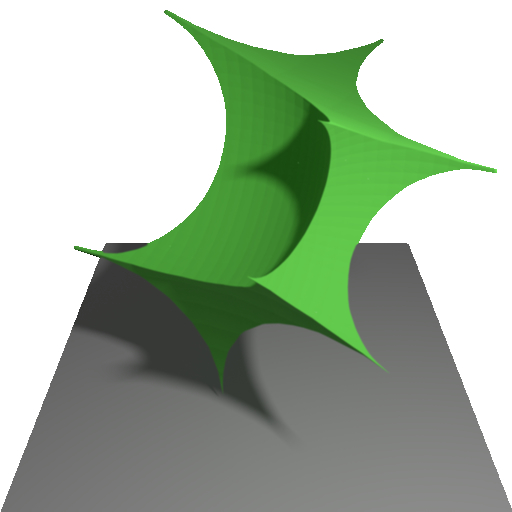
\includegraphics[height=1.2in, keepaspectratio]{./img/introduction/cube.jpg}
   \caption{Cube-type sphairahedron.}
   \label{fig:cubeSphaira}
  \end{minipage}
  \hspace*{\fill}
 \begin{minipage}[t]{0.75\textwidth}
  \begin{minipage}[t]{0.25\textwidth}
   \centering
   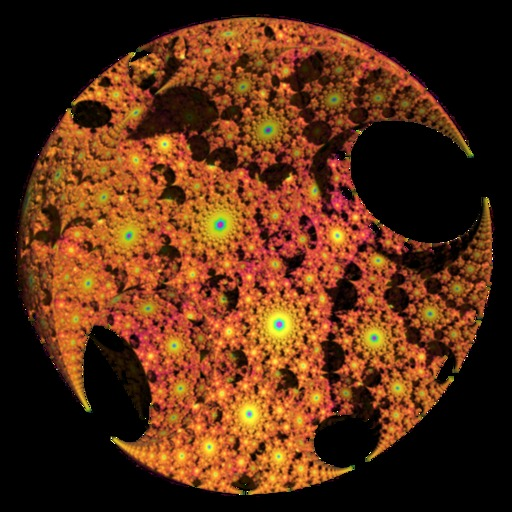
\includegraphics[height=1.2in,
   keepaspectratio]{./img/introduction/quasi-sphere.jpg}
   \subcaption{}
  \end{minipage}
  \hspace*{\fill}
  \begin{minipage}[t]{0.25\textwidth}
   \centering
   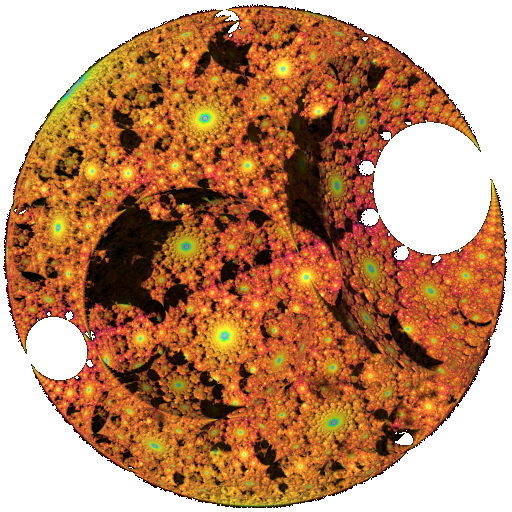
\includegraphics[height=1.2in,
   keepaspectratio]{./img/introduction/other.jpg}
   \subcaption{}
  \end{minipage}
  \hspace*{\fill}
  \begin{minipage}[t]{0.25\textwidth}
   \centering
   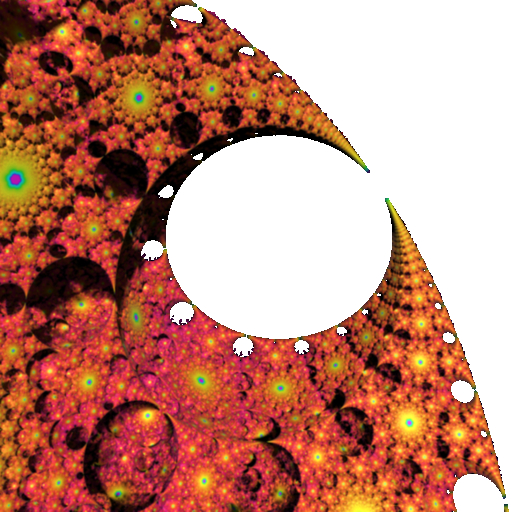
\includegraphics[height=1.2in,
   keepaspectratio]{./img/introduction/quasi-sphereZoom.jpg}
   \subcaption{}
  \end{minipage}
  \hspace*{\fill}
  \caption{Images of a quasi-sphere rendered in different viewpoints.}
  \label{fig:quasi-sphere}
 \end{minipage}
\end{figure}

\subsection{Background}

The main target of this paper is a visualization of four-dimensional
Kleinian groups, which is a discrete subgroup of the isometry group of
that four-hyperbolic space $H^4$. A four-dimensional Kleinian group $G$ acts
on $S^3$, the boundary of $H^4$ as a M\"obius transformation on
$S^3$. \par
We have few studies about a finitely generated M\"obius group on $S^3$,
and we start at a group arising from a sphairahedron introduced by Ahara
and Araki in 2003\cite{AharaAraki}.
Sphairahedron is a coined word combining two words 'sphaira' (a prefix
that means 'spherical') and 'hedron' (a suffix comes from 'polyhedron.')
It looks like a polyhedron, but each face is a part of a sphere. See
Figure \ref{fig:cubeSphaira}. It shows a cube-type sphairahedron. The
polyhedral structure of the sphairahedron coincides with that of a cube.

We consider a group $G$ generated by the inversion of the six faces. An
inversion is an orientation reversing isometry. Thus we consider an
extended M\"obius transformation group; that is, we include both
orientation preserving and orientation reversion M\"obius transformations
and $\text{M\"ob}(S^3)$ denotes a group generated by all
sphere-inversions in $S^3$.

$G$ may give a tiling by closed sphairahedra in $S^3$. In some cases, the
boundary of the tiling patterns converges to a three-dimensional fractal
configuration. This boundary is the limit set of $G$. If it is
homeomorphic to a two-dimensional sphere $S^2$, we call it
\textit{quasi-sphere} and the group $G$ a quasi-fuchsian group. We show
an example of a quasi-sphere in Figure \ref{fig:quasi-sphere}.

Ahara and Araki published graphics and mathematical theories about a sphairahedron
and a quasi-sphere in ICG 2002, that is, an international conference about
computer graphics. 
The paper introduces mathematical background than the way of the rendering
graphics and the simplest parameter space of cube-type sphairahedra
with the graphics rendered by POV-Ray.
After that, Ahara presented the paper written in Japanese\cite{AharaJa}
,showing the varieties of sphairahedra and dimensions of parameter space.
In 2016, Ryo Kageyama\cite{kageyama} decided the parameter space of the cube type
sphairahedron, and moreover, introduced varieties of deformations of
quasi-spheres.

In the graphical aspect, in 2012, Knighty developed a script to render
quasi-spheres in real-time under limited conditions
\footnote{\url{http://www.fractalforums.com/ifs-iterated-function-systems/another-3d-kleinian/}}.
In 2014, J\'er\'emie Brunet published a book of
fractal paintings named ``L'art fractal''. One of the works in the book called
``Quasi-Quasi-Grail'' is based on Ahara and Araki fractal.

After that, in 2017, a breakthrough came out. 
Nakamura and Ahara developed an algorithm called
\textit{Iterated Inversion System (IIS)}\cite{bridges2016}\cite{bridges2017}.
We combine IIS and Sphere tracing, which is a kind of ray tracing
techniques; we can render quasi-spheres dramatically fast.
IIS is the way to render CG related to a finitely generated group
generated by symmetry transformations and inversions pixel by pixel.
It can be easy to parallelize and render an image fast. 
Rendering quasi-sphere using IIS and sphere tracing is published in
Bridges\cite{bridges2018}, an international conference about mathematics
and arts.
This shows not only the way for CG but also an algorithm for mathematical art.

Note that there are many pictures of three-dimensional, so it is hard to
see the whole appearance only by them. We can see sphairahedron based
fractal renderer, more pictures, and more movies in
our web site\footnote{\url{https://sphairahedron.net}}.

In this paper, we aim for to the following purposes.
First, we survey the history of these quasi-spheres.
Second, we rearrange the paper about the parameter space of sphairahedra
written in Japanese and report the comprehensive result.
Third, we properly introduce and prove mathematical theory implicitly
used for CG until now.
Fourth, we introduce the software to render sphairahedron developed by
Nakamura and the unsolved problems. 

\section{Preparation}

\subsection{sphairahedron}
\begin{figure}[h!tbp]
  \begin{minipage}[t]{0.3\textwidth}
   \centering
   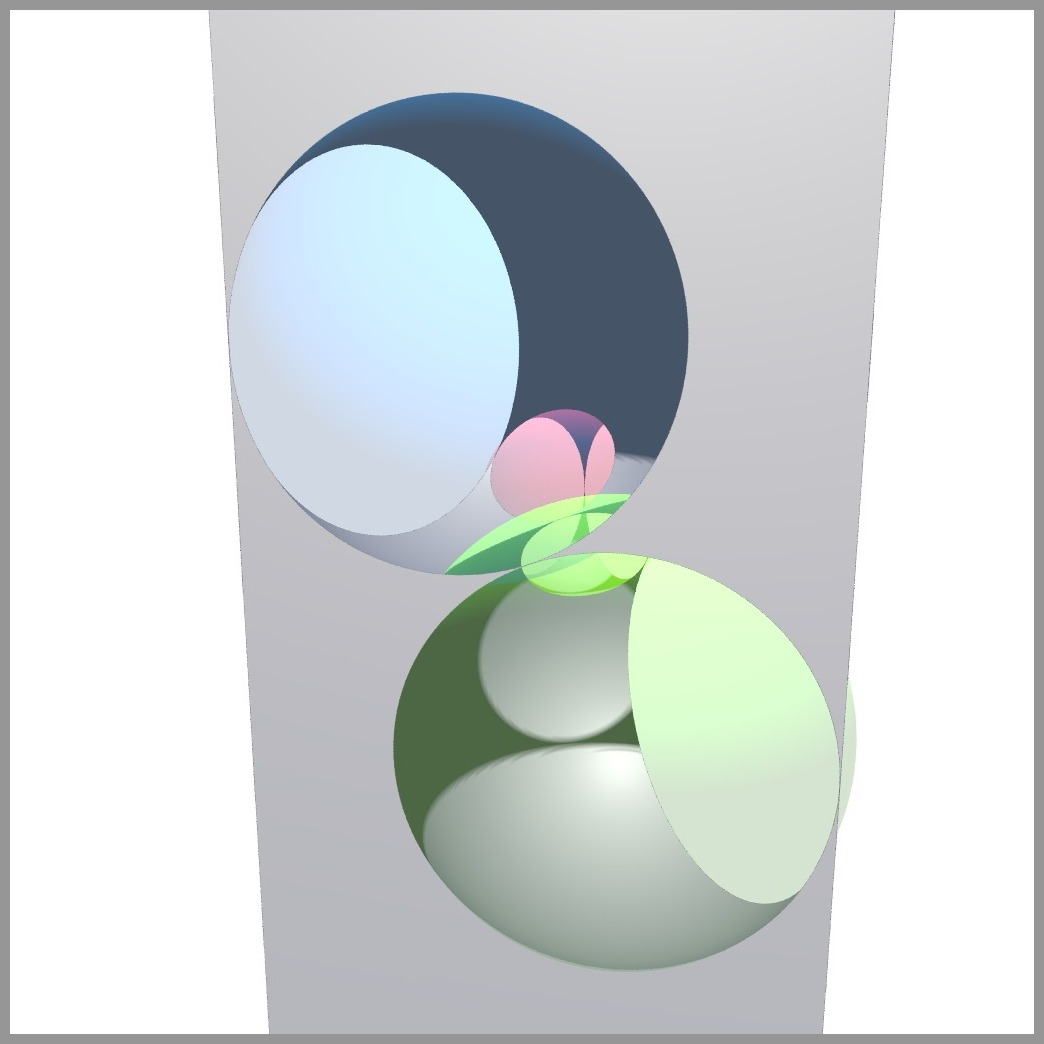
\includegraphics[width=1.2in, height=1.2in, keepaspectratio]
   {./img/sphairahedralPrism/sphairaAll.jpg}
   \subcaption{$A$}
   \label{fig:sphairaPrismAll}
  \end{minipage}
  \hspace*{\fill}
  \begin{minipage}[t]{0.3\textwidth}
   \centering
   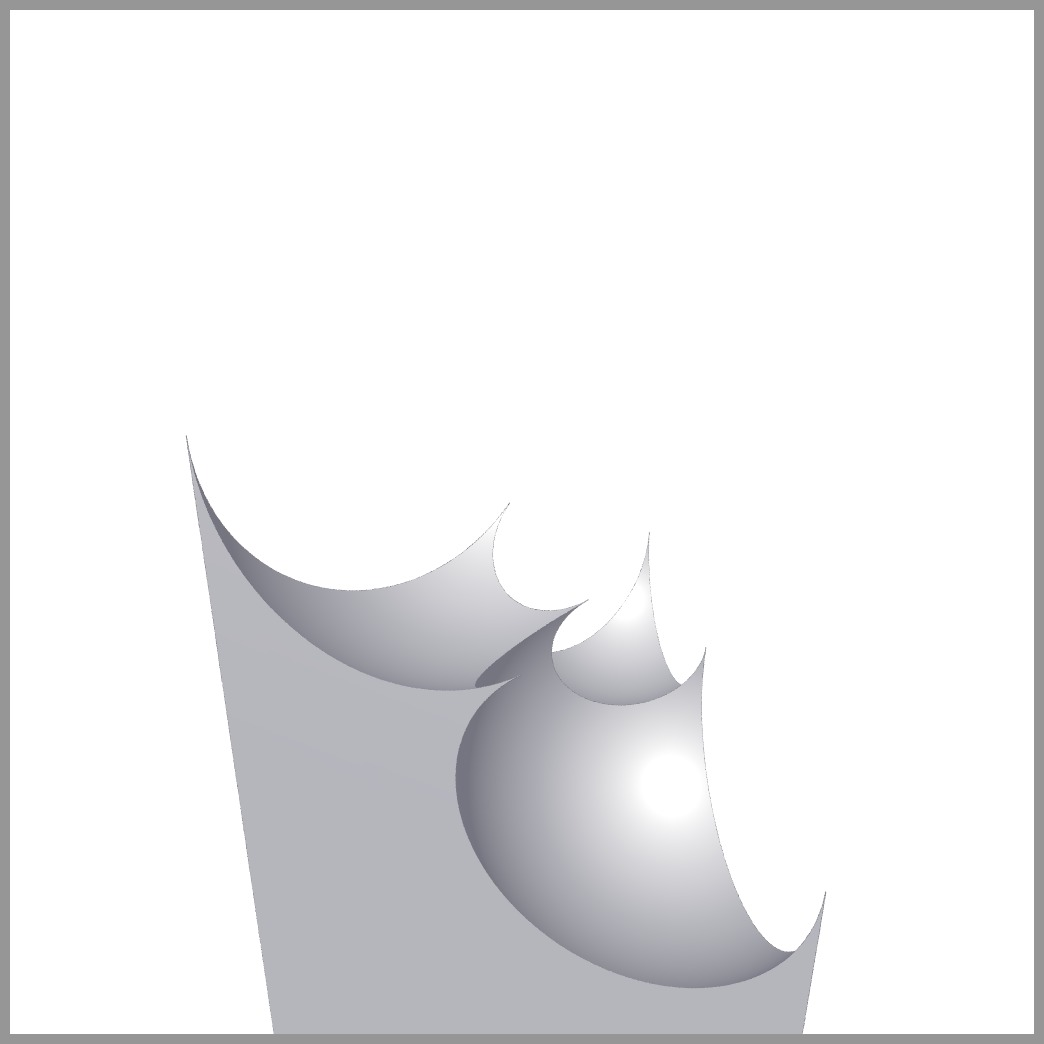
\includegraphics[width=1.2in, height=1.2in, keepaspectratio]
   {./img/sphairahedralPrism/sphairaHalf.jpg}
   \subcaption{Infinite type}
   \label{fig:sphairaPrismHalf}
  \end{minipage}
  \hspace*{\fill}
  \begin{minipage}[t]{0.3\textwidth}
   \centering
   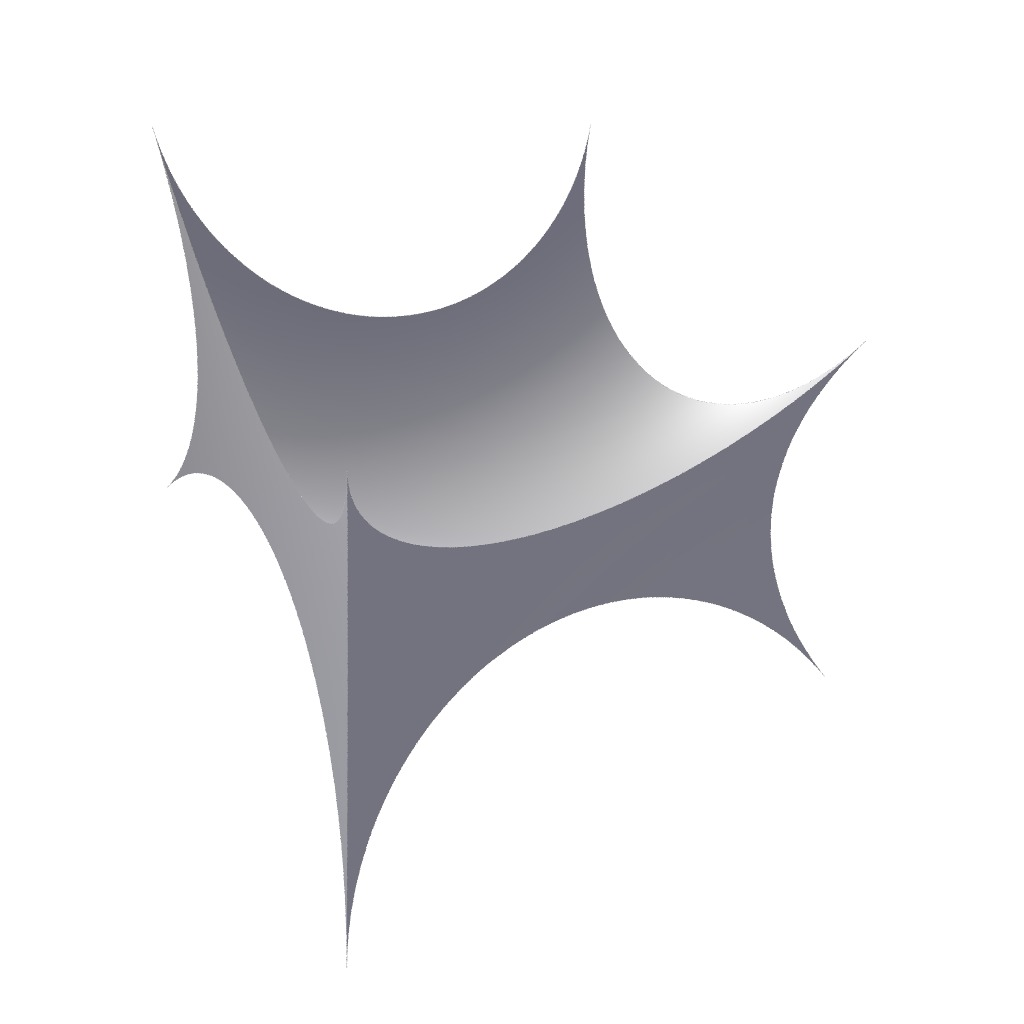
\includegraphics[width=1.2in, height=1.2in,
   keepaspectratio]{./img/sphairahedralPrism/sphairahedron.jpg} 
   \subcaption{Finite type}
   \label{fig:sphairahedronFinite}
  \end{minipage}
  \hspace*{\fill}
  \caption{Sphairahedron.}
  \label{fig:sphairahedron}
 \end{figure}

\begin{figure}[h!tbp]
 \begin{minipage}[t]{0.6\textwidth}
  \begin{minipage}[t]{0.3\textwidth}
   \centering
   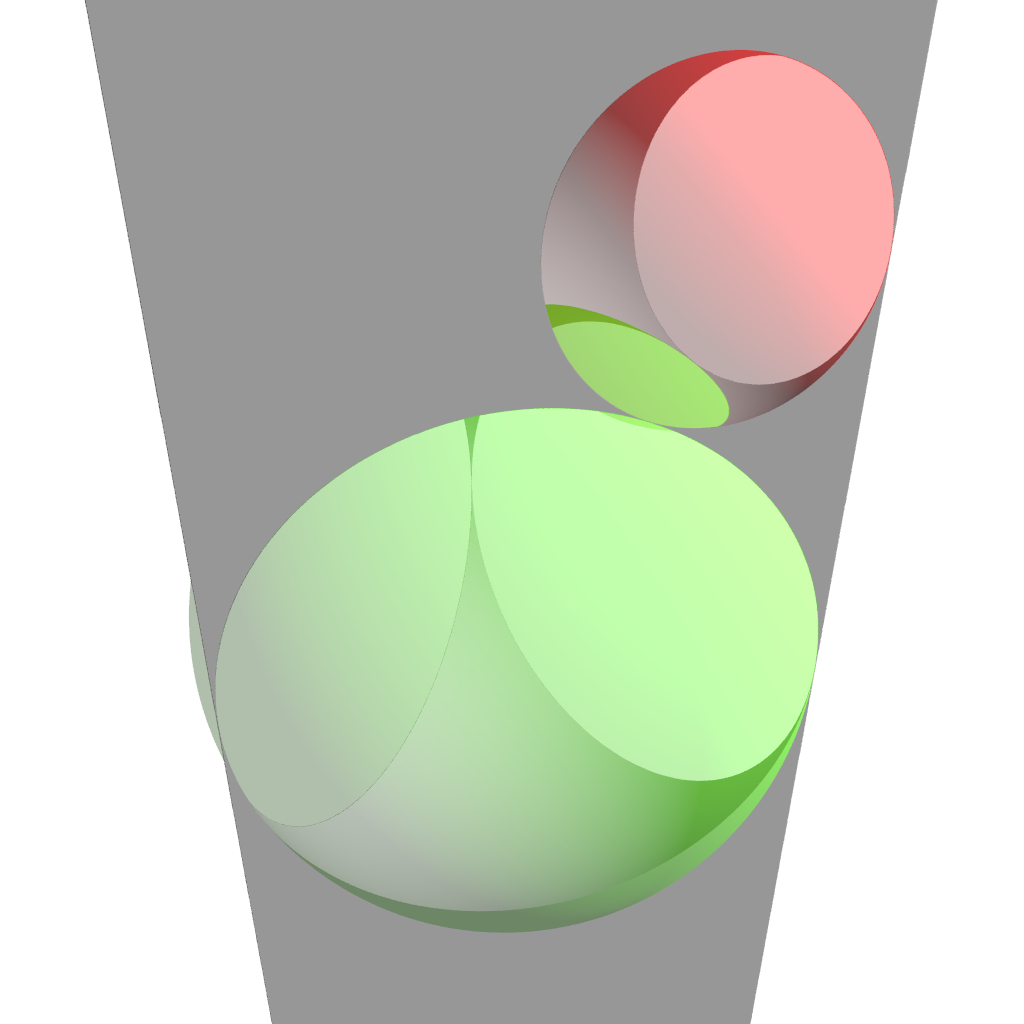
\includegraphics[width=1.2in, height=1.2in,
   keepaspectratio]{./img/sphairahedralPrism/semiSphairaAll.jpg}
   \subcaption{$A$}
   \label{fig:semi-sphairaAll}
  \end{minipage}
  \hspace*{\fill}
  \begin{minipage}[t]{0.3\textwidth}
   \centering
   
\includegraphics[width=1.2in, height=1.2in,
   keepaspectratio]{./img/sphairahedralPrism/semiSphairaHalf.jpg}
   \subcaption{Infinite type}
   \label{fig:semi-sphairaHalf}
  \end{minipage}
  \hspace*{\fill}
  \caption{Semi-sphairahedron.}
  \label{fig:semi-sphairahedron}
 \end{minipage}
 \begin{minipage}[t]{0.3\textwidth}
  \centering
 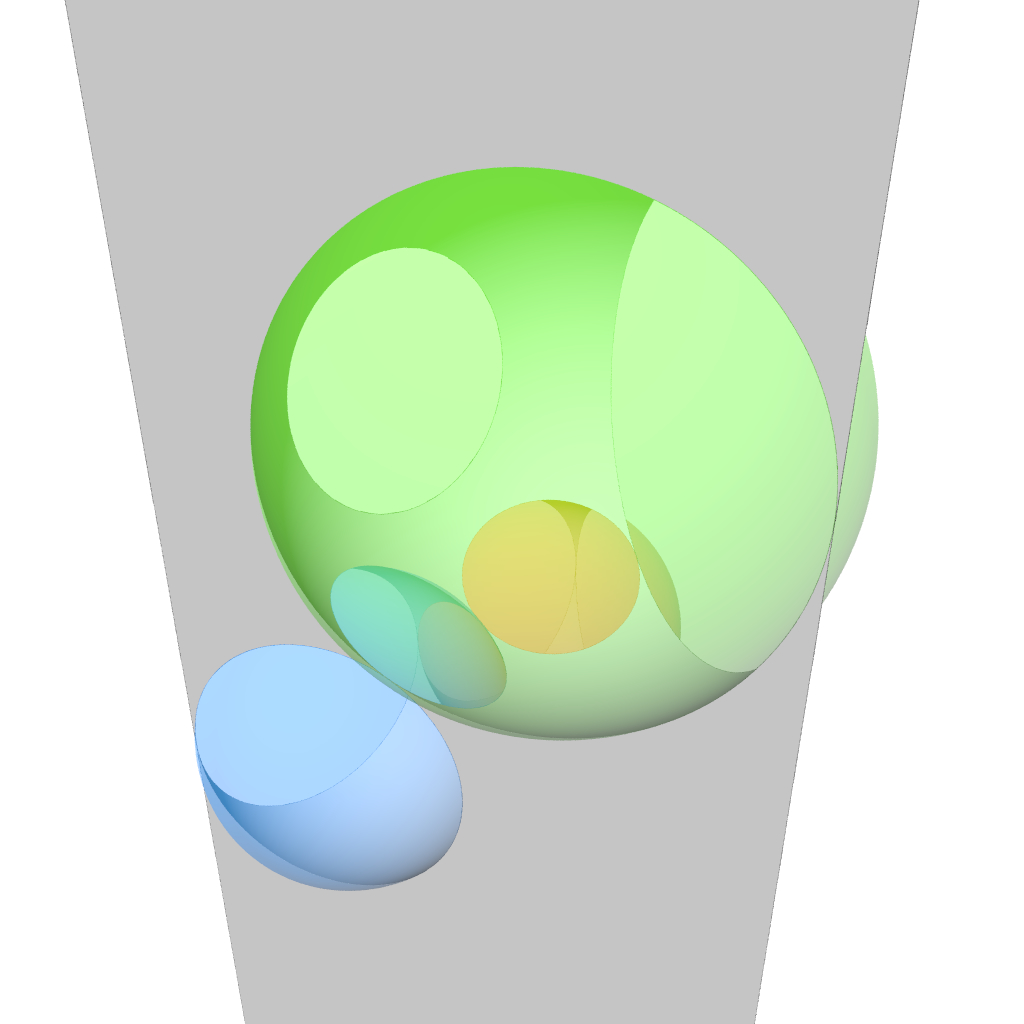
\includegraphics[width=1.2in, height=1.2in,
 keepaspectratio]{./img/sphairahedralPrism/hole.jpg}
 \caption{sphairahedron with hole.}
  \label{fig:brokenHole}
 \end{minipage}
\end{figure}

We will describe the simple definition of a sphairahedron used in \cite{bridges2018}.
\begin{definition}
Let $S^3 = R^3 \cup \{\infty\}$ be a three-dimensional sphere and let
$\overline{D_1},~\overline{D_2},\ldots,~\overline{D_p}$ be
three-dimensional closed balls or closed half-spaces in $S^3$.
We consider the complement $A$ of the union of these balls, that is,
$A = S^3 \setminus (\overline{D_1} \cup \overline{D_2} \cup ... \cup \overline{D_p})$.
If $A$ consists of two components and all components are simply-connected,
we call a component of $A$ a sphairahedron.
\end{definition}
The image in Figure \ref{fig:sphairahedron}\subref{fig:sphairaPrismAll}
is an example of a sphairahedron. 

Because of that definition, a sphairahedron has faces, edges, and
vertexes. We define \emph{ideality} and \emph{rationality} of a spairahedron.

\begin{definition}
(1)\ Let $S$ be a sphairahedron.  For each vertex, if all edges passing through the vertex are tangential to each other, we all it an \emph{ideal} sphairahedron.\par 
(2)\ Let $S$ be a sphairahedron.  For each edge, if the dihedral angle at the edge is rational (that is, the angle equals to $\pi/n$, where $n$ is a natural number,) we call it an \emph{rational} sphairahedron.
\end{definition}

In the sequel, we mainly consider a ideal rational spairahedron.  
When one of the vertexes is the infinity-point $\infty$ of $S^3$,
we call the sphairahedron \textit{infinite sphairahedron}.
One example is shown in Figure
\ref{fig:sphairahedron}\subref{fig:sphairaPrismHalf}.
Here, we consider a triangular prism with infinitely length and we hollow
out it by three balls, and select one of the connected components as a  sphairahedron.  At infinite, a face adjacent to the infinite vertex is a plane, the boundary of the half space.  Thus the neighborhood of the infinite vertex is a prism.

When the closure of a sphairahedron does not contain the infinite point,
we call it \textit{finite sphairahedron}.
See Figure\ref{fig:sphairahedron}\subref{fig:sphairahedronFinite}.

%--------
% We hollow out the $S^3$ with six balls: we remove three half-spaces
% (three balls with infinite radius,) from $S^3$ and obtain the prism of
% infinite length, and we scoop out the prism by the remaining
% three-colored transparent balls as in Figure
% \ref{fig:sphairahedron}\subref{fig:sphairaPrismAll}.
% $A$ is composed of two parts, and each of the components is simply connected.
% Since it has six faces, and these faces are arranged as those of faces of
% a cube, it is called a cube-type sphairahedron.
% Especially, the sphairahedron showned in Figure 
% \ref{fig:sphairahedron}\subref{fig:sphairaPrismHalf}
% is also called an \textit{infinite type sphairahedron},
% because one of the vertexes of the sphairahedron is at the infinity.
% Similarly, the shape hollowed out by six finite balls in Figure
% \ref{fig:sphairahedron}\subref{fig:sphairahedronFinite} is called a
% \textit{finite type sphairahedron}.
%---------- 

Moreover, we can loosen the definition of an ideal rational sphairahedron, 
that is, we allow the case $A$ has simply connected three or more components.

\begin{definition}
Let $\overline{D_1}, \overline{D_2},\ldots, \overline{D_p}$ be ball or
half-space in $S^3$.  If the complement $A$ of the unions of
$\overline{D_i}$'s has more than two connected components and all
components are simply connected, we call one component (or the union of
touching two (or more) components) a semi-sphairahedron.
\end{definition}
Figure \ref{fig:semi-sphairahedron}\subref{fig:semi-sphairaAll} shows an
example of a ideal rational semi-sphairahedron.  We can get this shape by scooping a
triangle prism out by two balls.  Complement $A$ consists of three
connected components. Lower two of them are tetrahedra, and the upper 
one is a pentahedron.  If we $T$ be the unions of lower two components,  
then $T$ is a semi-sphairahedron and we can regard it as a spairahedron with a singular point.  See Figure \ref{fig:semi-sphairahedron}\subref{fig:semi-sphairaHalf}.


Remark that Ahara, Araki\cite{AharaAraki}.,
and Kageyama\cite{kageyama} did not deal with semi-sphairahedra and their rendering images.

Other than semi-sphairahedra, we have much more 'sphairahedron-like
shapes' in the ideal and rational situation.  See Figure \ref{fig:brokenHole}. In this
figure, we see a hole at one of the faces.  This shape does not generate a
sphairahedron, but we can apply the tiling method in the below section, 
and we have a (non-simply-connected) limit set.  We have not classified
these figures mathematically yet, but possibly it occurs some
interesting geometry problems from here.


\subsection{Limit set}\label{constructFractal}

\begin{figure}[H]
 \begin{minipage}[t]{0.18\textwidth}
  \centering
  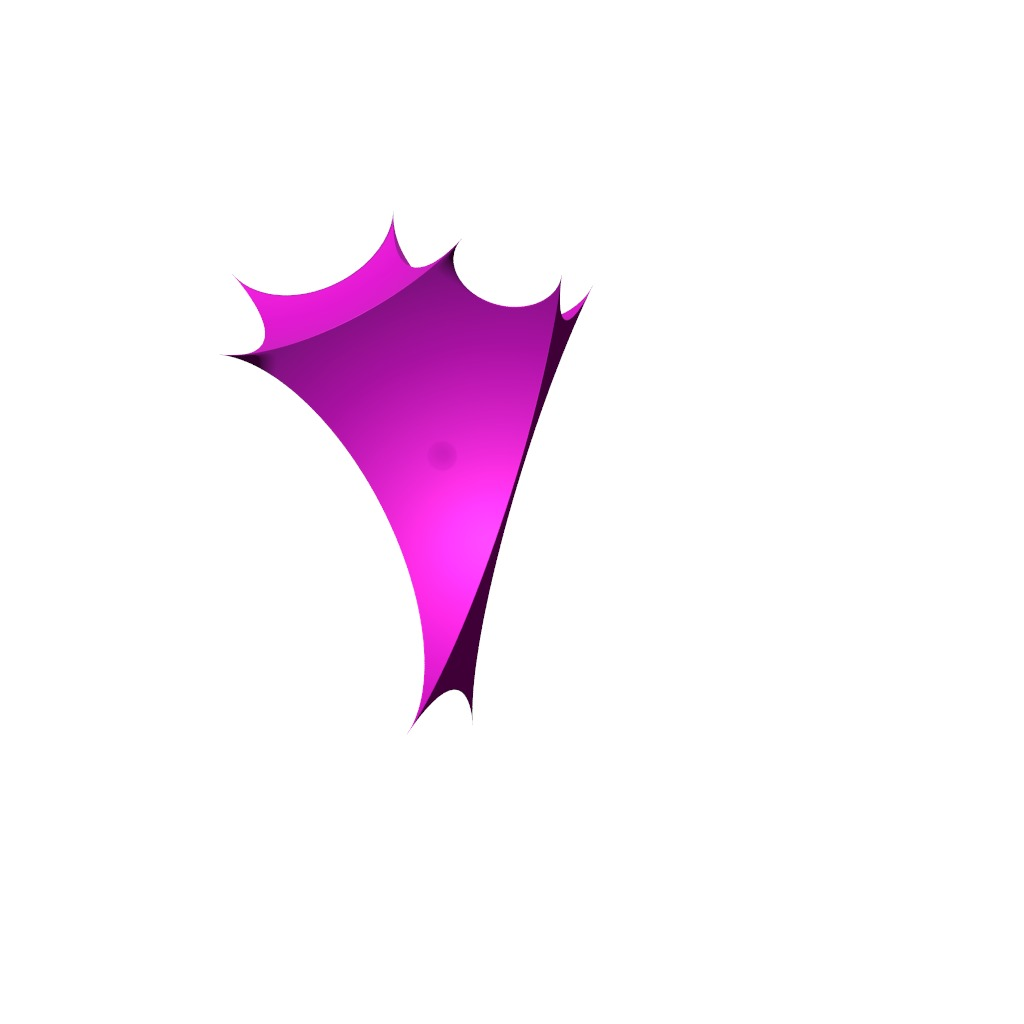
\includegraphics[width=1in, height=1in, keepaspectratio]{./img/constructFractal/finiteProcess/step1.jpg}
  \subcaption{Step 0}
  \label{fig:sphaira-step1}
 \end{minipage}
 \hspace*{\fill}
 \begin{minipage}[t]{0.18\textwidth}
  \centering
  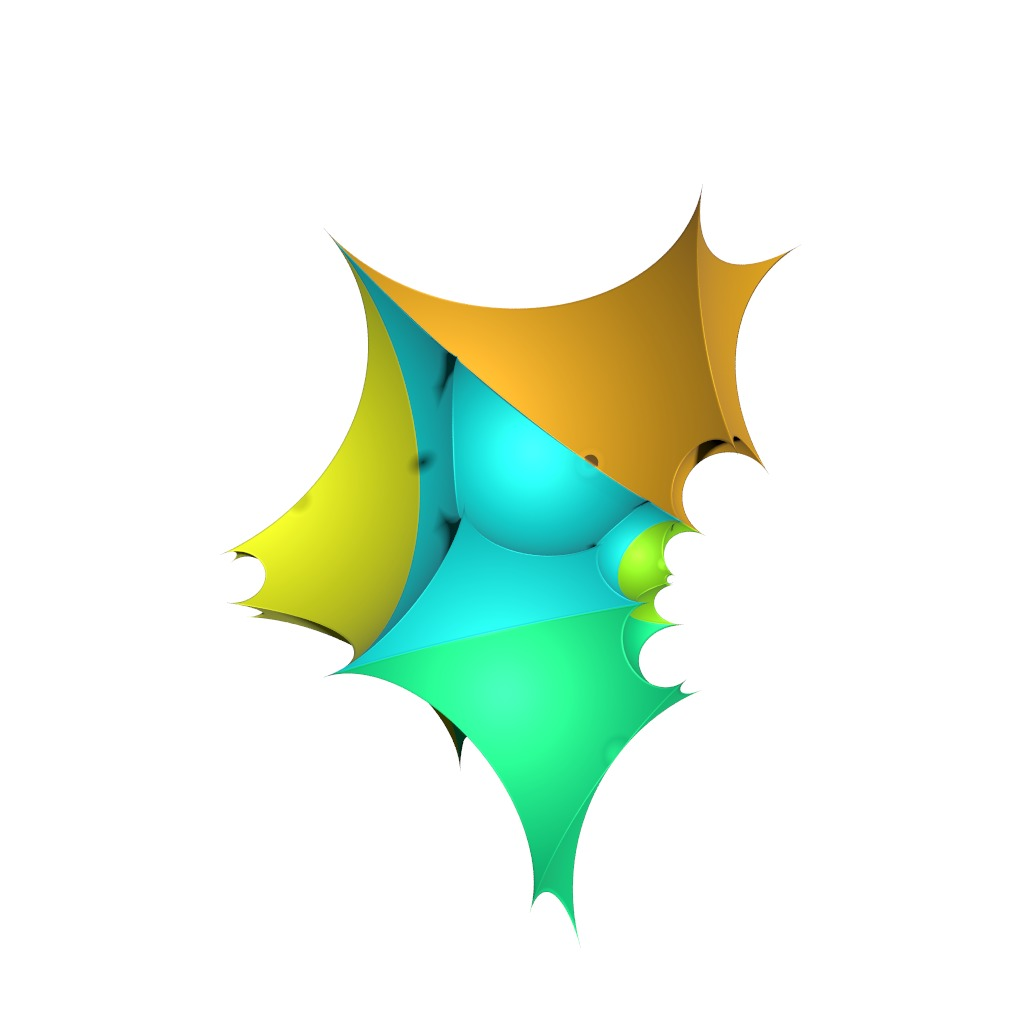
\includegraphics[width=1in, height=1in, keepaspectratio]{./img/constructFractal/finiteProcess/step2.jpg}
  \subcaption{Step 1}
  \label{fig:sphaira-step2}
 \end{minipage}
 \hspace*{\fill}
 \begin{minipage}[t]{0.18\textwidth}
  \centering
  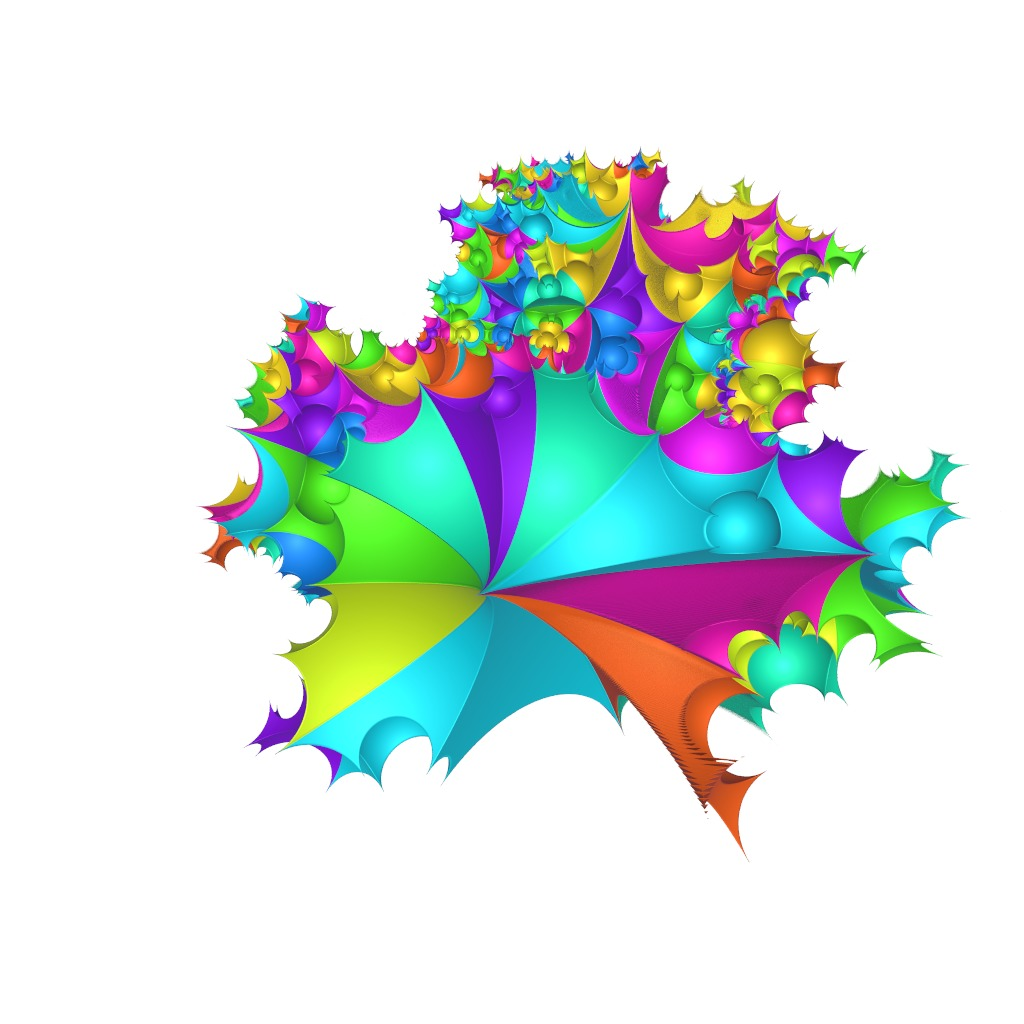
\includegraphics[width=1in, height=1in, keepaspectratio]{./img/constructFractal/finiteProcess/step5.jpg}
  \subcaption{Step 5}
  \label{fig:sphaira-step5}
 \end{minipage}
 \hspace*{\fill}
 \begin{minipage}[t]{0.18\textwidth}
  \centering
  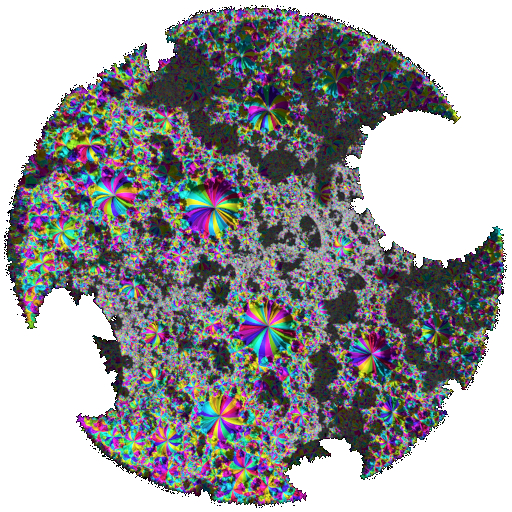
\includegraphics[width=1in, height=1in, keepaspectratio]{./img/constructFractal/finiteProcess/step10.jpg}
  \subcaption{Step 10}
  \label{fig:sphaira-step10}
 \end{minipage}
 \hspace*{\fill}
 \begin{minipage}[t]{0.18\textwidth}
  \centering
  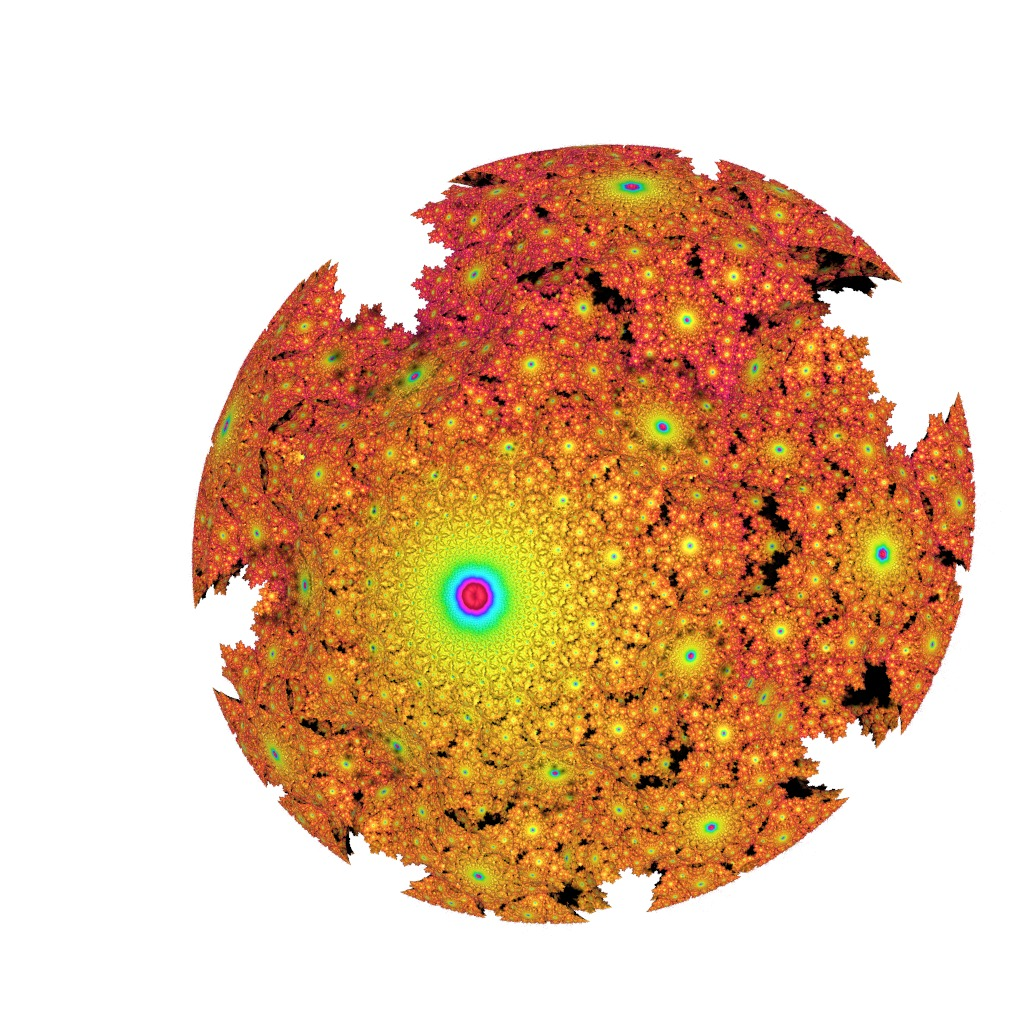
\includegraphics[width=1in, height=1in, keepaspectratio]{./img/constructFractal/finiteProcess/final.jpg}
  \subcaption{Final image}
  \label{fig:sphaira-final}
 \end{minipage}
 \hspace*{\fill}
 \caption{Tiling of a finite cube-type sphairahedron.}
 \label{fig:sphairahedronTile}
\end{figure}

Let $T$ be a sphairahedron.  Let $\overline{D_i}$ ($i = 1,2,\ldots, p$) be the closed ball of $T$ and $S_i$ be the boundary sphere of $\overline{D_i}$.  Suppose that a map $\varphi_i:S^3 \to S^3$ is the inversion map of $S_i$.  $\varphi_i$ is an orientation-reversing M\"obius map on $S^3$ and let $G$ be a group generated by all $\varphi_i$'s.  That is,
\[
 G := \langle\varphi_1, \varphi_2, \ldots , \varphi_p  \rangle < \text{Mob}(S^3)
\]

For a subgroup $G$ of
$\text{Mob}(S^3)$, let the discontinuity set $\Omega(G)$ be
\[
\Omega(G) = \left\{ x \in S^3 \left| \hspace{1mm} 
\begin{minipage}{8cm}
the point $x$ possesses a neighborhood $U(x)$
such that the intersection $U(x) \cap gU(x)$ is empty for all but finite
elements $g\in G$
\end{minipage}
 \right. \right\}.
\]
The complement $\Lambda(G) := S^3 \backslash \Omega(G)$ is called the
limit set of the group $G$. $G$ is a (4 dimensional) Kleinian group if $\Omega(G)$ is
not empty\footnote{Usually we consider a Kleinian group as a discontinuous subset of the orientation preserving M\"obius transformation group $\text{Mob}_+(S^3)$, however we relax the condition of orientation preserving.}. The limit set $\Lambda(G)$ consists either of 0 or 1 or 2 or
infinitely many points. Here we consider only the case that $\Lambda(G)$
is infinite and two-dimensional. 
A Kleinian group $G$ is called a
3-Kleinian group if $\Lambda(G)$ is a round sphere. This means that $G$ can be reduced into the Kleinian group $\text{Mob}(S^2)$ in the usual sense.  
A Kleinian group $G$ is called a
quasi-fuchsian group if $\Lambda(G)$ is homeomorphic to a closed sphere, 
and there exists a homeomorphism $f:S^3 \rightarrow S^3$ which conjugates
$G$ to a 3-Kleinian group. If $G$ is a quasi-fuchsian group, the limit set
$\Lambda(G)$ may be a fractal sphere, that is, a sphere embedded in $S^3$ with
 fractal structure.

%球面体をタイリングすることができる。(ポアンカレの多面体定理)
Let $L$ be the tiling generated by a tile $T$ and a transform group $G$, that is, the piece set of $L$ consists of $g(T)$ for all $g\in G$.  We represent $L$ by the pair $(T,G)$.  The rationality condition guarantees the local consistency of tiling satisfies because of Poincare's polyhedron theorem.  

%実際に、群$G$の長さが短い要素から考えていくと、その和集合はローカルには球体と同相な図形の$S^3$へのはめ込み(局所的な埋め込み)になる。
Let $|L|_k$ be the union of tiles $g(\text{Closure}(T))$ such that the word length of $g\in G$ is less than $k+1$.  At least for a small $k$, $|L|_k$ is homeomorphic to a 3-ball $B^3$.  For a large $k$ there are no guarantee to be a 3-ball, though if we consider the universal covering $\widetilde{|L|_k}$ of the union of tiles, $\widetilde{|L|_k}$ is a ball for any $k$.  There is a natural immersion $i_k:\widetilde{|L|_k}\to|L|_k\subset S^3$.  The tiling $L=(T,G)$ is {\it embedded} in $S^3$ if the immersion $i_k$ is an embedding for any $k$.  Whether a given tiling $L$ can be embedded in $S^3$ depends on the shape of the fundamental sphairahedron $T$ and it is not trivial to show this.  

Using sphairahedron.net\cite{sphairahedron_net}, we can observe rendered images of $|L|_k$.  See Figure \ref{fig:sphairahedronTile}.   In Figure
\ref{fig:sphairahedronTile}\subref{fig:sphaira-step1} we see the fundamental sphairahedron with six faces.  $|L|_1, |L|_5, |L|_{10}$ is shown in Figure
\ref{fig:sphairahedronTile}\subref{fig:sphaira-step2}\subref{fig:sphaira-step5}\subref{fig:sphaira-step10}.  In these figure, adjacent tiles have different colors.  In Figure \ref{fig:sphairahedronTile}\subref{fig:sphaira-step10}, outside tiles are so small and we see the union in gray color.  These figures suggest us that $|L|_k$'s are embedded in $S^3$.  Figure \ref{fig:sphairahedronTile}\subref{fig:sphaira-final} shows a rendering image for a large enough $k$.  In this figure we use another algorithm to render the image shown in *** and we success to color the shape properly.

We show another example of $|L|_k$ in Figure \ref{fig:sphairahedralPrismTile}.  In this example the fundamental tile is an infinite sphairahedron.  The resulting shape in Figure \ref{fig:sphairahedralPrismTile}\subref{fig:sphairaPrismFinal} looks like a terrain of scenic beauty.

Here we present a conjecture after observation of the simulations by sphairahedron.net\cite{sphairahedron_net}.

\begin{conjecture}
If $T$ is an ideal rational sphairahedron, the tiling $L=(T,G)$ is embedded in $S^3$.
\end{conjecture}

Here we see the limit set of the group $G$.  In fact it is well-known that the limit set is the closure of the accumulation point set of an orbit.  Using this characteristic, we have the following.

\begin{lemma}
If the tiling $L=(T,G)$ is embedded in $S^3$, then we have
\[
\Lambda(G) =\partial(\varlimsup_{k\to\infty} |L|_k)
\]
\end{lemma}

\begin{figure}[h!tbp]
 \begin{minipage}[t]{0.18\textwidth}
  \centering
  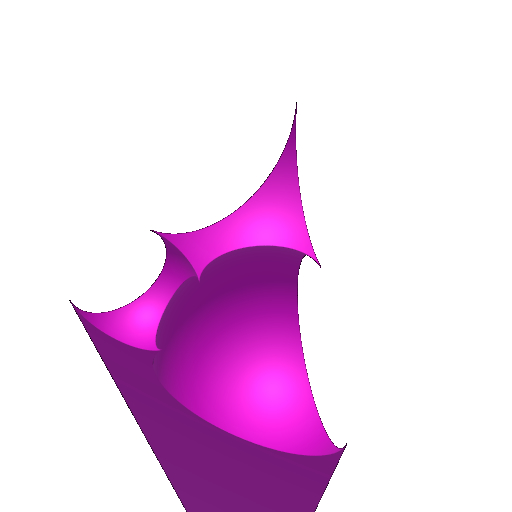
\includegraphics[height=1.1in, keepaspectratio]{./img/constructFractal/terrainProcess/step1.jpg}
  \subcaption{Step 1}
  \label{fig:terrainStep1}
 \end{minipage}
 \hspace*{\fill}
 \begin{minipage}[t]{0.18\textwidth}
  \centering
  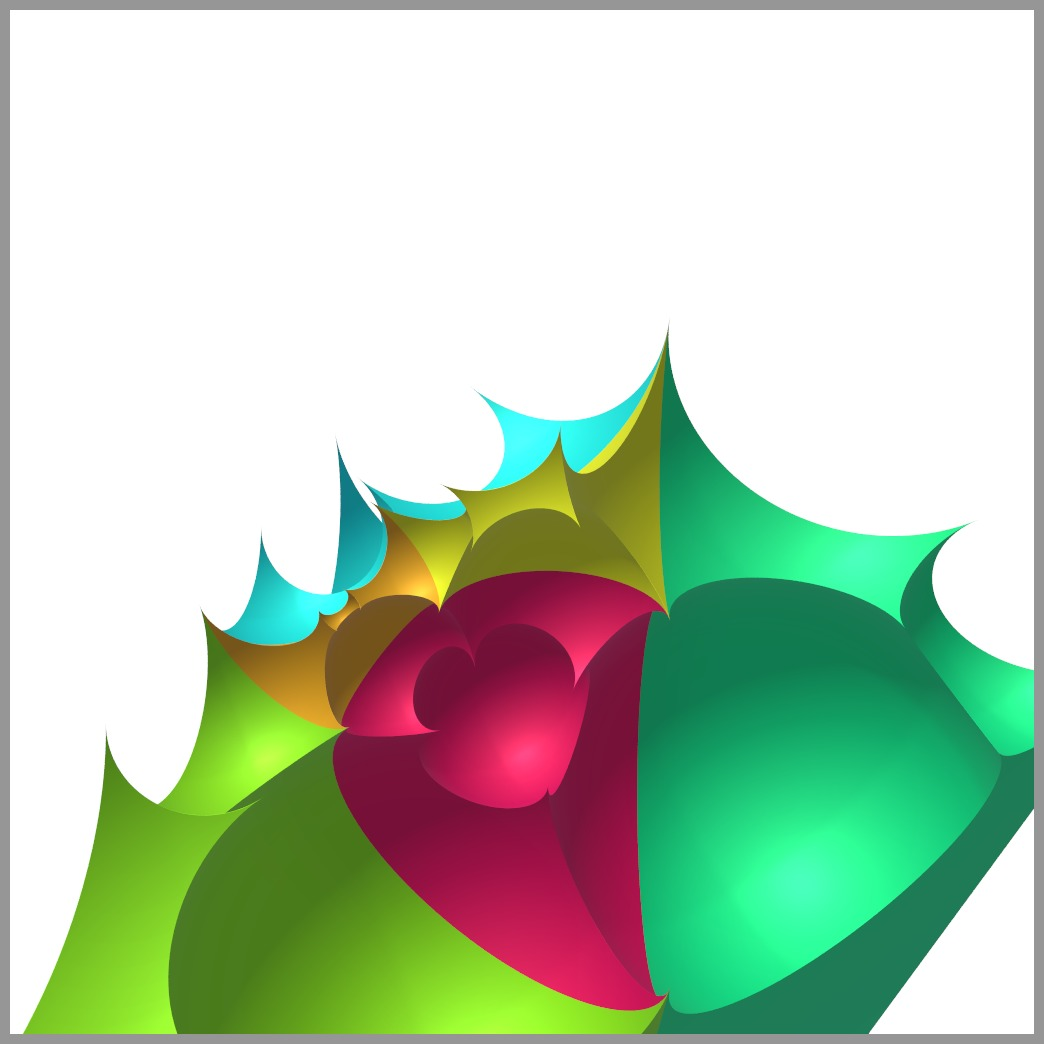
\includegraphics[height=1.1in, keepaspectratio]{./img/constructFractal/terrainProcess/step2.jpg}
  \subcaption{Step 2}
  \label{}
 \end{minipage}
 \hspace*{\fill}
 \begin{minipage}[t]{0.18\textwidth}
  \centering
  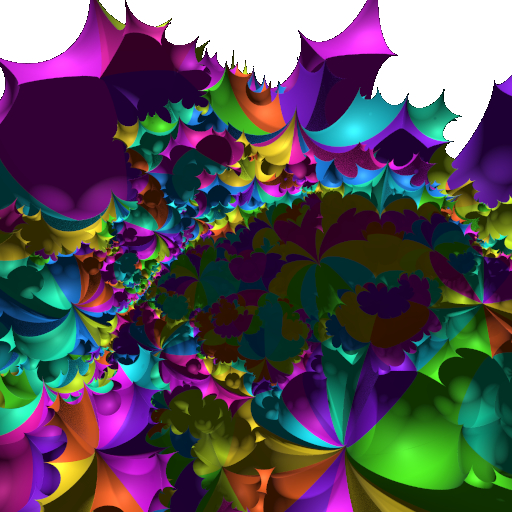
\includegraphics[height=1.1in, keepaspectratio]{./img/constructFractal/terrainProcess/step5.jpg}
  \subcaption{Step 5}
  \label{}
 \end{minipage}
 \hspace*{\fill}
 \begin{minipage}[t]{0.18\textwidth}
  \centering
  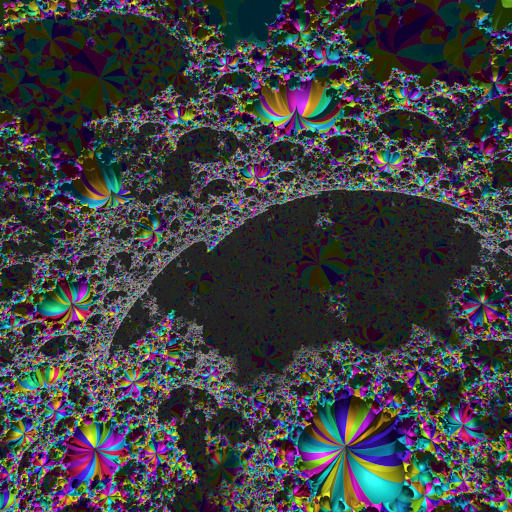
\includegraphics[height=1.1in, keepaspectratio]{./img/constructFractal/terrainProcess/step10.jpg}
  \subcaption{Step 10}
  \label{fig:terrainStep10}
 \end{minipage}
 \hspace*{\fill}
 \begin{minipage}[t]{0.18\textwidth}
  \centering
  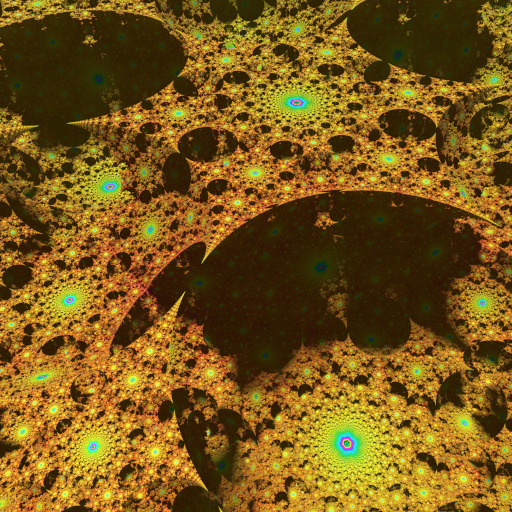
\includegraphics[height=1.1in, keepaspectratio]{./img/constructFractal/terrainProcess/final.jpg}
  \subcaption{Final image}
  \label{fig:sphairaPrismFinal}
 \end{minipage}
 \caption{Tiling of a cube-type infinite sphairahedron.}
 \label{fig:sphairahedralPrismTile}
\end{figure}

%semi-sphairahedronについてはここで書く。
In the same way as above, a semi-sphairahedron
can be tiled by the inversions of its faces.
Though the fundamental tile may be not connected and each $|L|_k$ is not connected nor the group is not quasi-fuchsian, the closure $\text{Closure}(|L|_k)$ is connected.  
See an example in Figure \ref{fig:semiSphairaSpheres}.  Here we see an plane and infinite number of balls touching to the ground and to each other.  Such shape can occur lower side of the plane, that is, we see only one plane but there are infinite number of spherical pitfalls underground.


\begin{figure}[h!tbp]
  \centering
 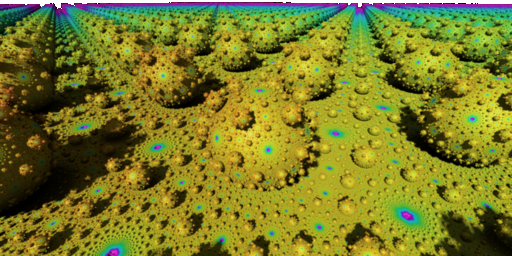
\includegraphics[width=2in,
 keepaspectratio]{./img/constructFractal/semi-terrain2.jpg}
 \caption{sphairahedron with hole.}
  \label{fig:semiSphairaSpheres}
\end{figure}

%%対称性については、「数学的知見」のところで扱う。
%Also, an infinite sphairahedron can be tiled, as presented in Figure
%\ref{fig:sphairahedralPrismTile}.
%The pattern converges to fractal terrain owing to reflections over side
%faces of the sphairahedron, as shown in Figure 
%\ref{fig:sphairahedralPrismTile}\subref{fig:terrainStep1}.
%In the fractal terrain, we can find symmetry easily.
%For example, we can see hexagram-like terrain patterns in Figure
%\ref{fig:sphairahedralPrismTile}\subref{fig:sphairaPrismFinal}.
%These patterns are originated from the dihedral angles of the side faces of
%$\pi / 3$.
%
%
%In the images of fractals within this paper, each tile of the
%sphairahedra is colored according to the
%number of inversions.
%We use the color wheel to determine their color,
%and the tile's color varies in order of red, yellow, green, and blue.
%In Figure \ref{fig:sphairahedronTile}\subref{fig:sphaira-step1} $\sim$ \subref{fig:sphaira-step10} and
%Figure \ref{fig:sphairahedralPrismTile}\subref{fig:terrainStep1} $\sim$ \subref{fig:terrainStep10},
%we refer color wheel with large steps to visualize each tile clearly.
%On the other hand, in the other images, we refer the wheel with smaller
%steps, and we find lots of tiles with many inversions in the blue
%parts of the fractal.

%Up to this point, we showed tiling patterns without gaps between the tiles and
%intersections of the tiles.
%However, not every sphairahedra can generate such proper tiling patterns.
%To obtain them, we have to consider two mathematical properties
%of the original sphairahedron. That is, the sphairahedron should be
%rational and ideal.
%In the following sections, we will introduce these properties and
%compute parameter space for the rational ideal sphairahedron.

\section{Parameter Spaces of Rational Ideal Sphairahedra}

\subsection{Classification of Sphairahedra}

%We are interested in finding examples of quasi-fuchsian sub-group of
%M\"ob$_{+}(S^3)$, the group of orientation preserving M\"obius
%transformation on $S^3 = R^3 \bigcup \{\infty\}$. 
%For a subgroup $G$ of
%Mob$_+(S^3)$, let the discontinuity set $\Omega(G)$ be
%$$
%\Omega(G) = \left\{ x \in S^3 \left| \hspace{1mm} 
%\begin{minipage}{8cm}
%the point x possesses a neighborhood $(x)$
%such that the intersection $U(x) \cap gU(x)$ is empty for all but finite
%elements $g\in G$
%\end{minipage}
% \right. \right\}.
%$$
%The complement $\Lambda(G) := S^3 \backslash \Omega(G)$ is called the
%limit set of the group $G$. $G$ is a Kleinian group if $\Omega(G)$ is
%not empty. The limit set $\Lambda(G)$ consists either of 0 or 1 or 2 or
%infinitely many points. Here we consider only the case that $\Lambda(G)$
%is infinite and two-dimensional. A Kleinian group $G$ is a fuchsian
%group if $\Lambda(G)$ is a closed round sphere. $G$ is called a
%quasi-fuchsian group is $\Lambda(G)$ is homeomorphic to a closed sphere, 
%and there exists a homeomorphism $f:S^3 \rightarrow S^3$ which conjugates
%$G$ to a fuchsian group. If $G$ is a quasi-fuchsian group, the limit set
%$\Lambda(G)$ may be a fractal sphere, that is, a sphere in $S^3$ with
%fractal structure.

%In two dimensional case, that is, $G$ is a subgroup of M\"ob$_+(S^2)$
%(or equivalently M\"ob$_+(H^3)$, we have many examples of quasi-fuchsian
%groups.) One of the important examples is a kissing Schottky group.
%Let $O_1^+, O_2^+, O_1^-, O_2^-$ be circles in $S^2$ such that
%$O_1^{\pm}$ are tangential to $O_2^{\pm}$. Let $f_i$ be a M\"obius
%transformation which maps the exterior of $O_i^+$ onto the interior of
%$O_i^{-}$ for $i = 1, 2$ and let a group $G$ be generated by $f_1, f_2$.
%(Remark that $\Lambda$ is homeomorphic to a circle if a set of the
%tangent points is equivalent under the action of $G$. See p.157 of
%\cite{indra}.)
%If the four circles are disjoint to each
%other, we call $G$ a Schottky group and $\Lambda(G)$ is an infinite set
%but is not homeomorphic to a circle. We may consider the case that
%$O_1^{\pm}$ intersects to $O_2^{\pm}$ by $\pi/n$ for a natural number
%$n$. In this case, we also have a circle-wise limit set $\Lambda(G)$.
%See p361 of \cite{indra}.

%The Coxeter-like group is another example. Consider 4 (or more) circles in
%$S^2$ (we call them 'initial circles.') Let $\tilde G$ be a group generated
%by the inversions of these initial circles. Here we assume that any two
%initial circles are disjoint or tangential or intersecting  by angle
%$\pi/n$ for $n \in N$. Then a subgroup $G$, which is defined by a set of
%all even-length-elements of $\tilde G$, is well-defined.
%
%In this article, we consider an extension of kissing Schottky groups and
%Coxeter-like groups to M\"ob($S^3$). In order to do that, we have to
%obtain a set of initial spheres (instead of 'initial circles') with some
%conditions. the following new problem of Euclidean geometry is
%one of the good approaches.

%\begin{problem}
% Let $S^3 = R^3 \bigcup {\infty}$. Find a polyhedron in $S^3$ satisfying
% the following conditions.
% \begin{description}
%  \item[Condition 1:] Each face of a polyhedron is a sphere in $S^3$.
%  \item[Condition 2 (rationality):] For each edge, the face-angle equals $\pi/n$
%             for a natural number $n$.
%  \item[Condition 3 (ideality):] For each vertex, edges with the vertex are
%             mutually tangent at the vertex.
% \end{description}
%\end{problem}

%In the following sections, we derive rational ideal sphairahedron.

In this section we consider ideal rational sphairahedra of various types. 
In order to classify such sphairahedra, we need three steps.  In the first step, we classify the polyhedral structure of a sphairahedron.  See Figure \ref{fig:tetrahedronFinite} for a tetraheron.  This example is a sphairahedron of tetrahedon type, this means that the polyhedral structure is same as that of a tetrahedron as in Figure \ref{fig:tetrahedronFaces}.  
In the second step, we classify combinations of dihedral angles of edges.  In tetrahedron case, there are three combinations as seen in Figure \ref{fig:tetrahedronCombinations}.  Here a number $n$ at each edge means that the dihedral angle at the edge is $\pi / n$. 
In the third step, we calculate the parameter space of the shape of sphairahedra.  Here we assume that two sphairahedra $T_1, T_2$ are equivalent if there exists a (orientation preserving/reversing) M\"obius transformation $f$ on $S^3$ such that $f(T_1) = T_2$.  In the tetrahedron case, the parameter space consists of only one point.  

%阿原荒木の仕事
Ahara and Araki \cite{AharaAraki} determine all of combinations of dihedral angles of the cube type sphairahedra and they show one of the parameter space without a proof.  
%阿原の仕事
Ahara \cite{AharaJa} determines all of polyhedral structures of sphairahedra with 5 or 6 faces.  He also shows the number of combinations of dihedral angles for each structure without a proof.  
Ahara and Araki \cite{AharaAraki2} determines all of the parameter spaces for the cube case with a proof.  This paper was quoted in other papers, however it is an unpublished preprint.
%影山さんの仕事(の関連部分)の紹介
Kageyama \cite{kageyama} introduces the result of \cite{AharaAraki2} without a proof. 
%この論文での守備範囲の紹介
In this paper, we introduce all of the parameter spaces of sphairahedra with 5 or 6 faces, including current results. The proof is so similar to that of \cite{AharaAraki2}, and we introduce it in the appendix.


%Usually, a polyhedron has planar faces. But easily, we can consider an
%extension of a polyhedron such that the faces are a part of a
%sphere. (Hence each edge is an arc.) If we have such polyhedron with
%the above conditions, we consider spheres of the faces as initial
%spheres. Easily we can consider a Coxeter-like group generated by the
%inversions of them.

%In this article, we first consider a polyhedron with the same cellular
%structure as that of a cube. (Hence the number of the initial spheres is
%6.) And we have the following result.

%\begin{theorem}\label{main}
% If a polyhedron with the above conditions is of cube-type (that is,
% the one skeleton of the polyhedron is the same as that of a cube), then
% there are seven combinations of face-angles. For each combination of
% face-angles, a set of conformal equivalent classes of polyhedra is two
% dimensional.
%\end{theorem}

%Once we have a polyhedron $P$ with the above conditions, we may consider
%a Coxeter-like subgroup $G=G(P)$ of M\"ob$_+(S^3)$. Through proving this
%theorem, we obtain that for each combination of dihedral angles, there is a
%polyhedron such that the limit set $\Lambda(G)$ is a round sphere. So,
%other polyhedra give us quasi-fuchsian groups. So we get a family of
%a quasi-fuchsian group with two parameters. At the same time, we have a
%family of fractal spheres with two parameters.

% This paper is organized as follows. In the section 2 we will show the
% above theorem. In the section 4 we consider other type
% of polyhedra and show a similar theorems.

We prepare some lemmas to execute classifications.

\begin{lemma}\label{sum}
Suppose that there are $k$ edges with a vertex. Then the sum of
 dihedral angles of these three edges is $(k-2)\pi$.  If $k=3$ then the combination of dihedral angles is 
one of $\left( \frac{\pi}{3}, \frac{\pi}{3}, \frac{\pi}{3}\right)$, $\left( \frac{\pi}{2}, \frac{\pi}{4}, \frac{\pi}{4}\right)$, and $\left( \frac{\pi}{2}, \frac{\pi}{3}, \frac{\pi}{6}\right)$.
If $k=4$ then the combination of dihedral angles is 
$\left( \frac{\pi}{2}, \frac{\pi}{2}, \frac{\pi}{2}, \frac{\pi}{2}\right)$. The case $k>4$ cannot happen.
\end{lemma}

\begin{proof}
 Let $\phi$ be a M\"obius transformation such that it maps the vertex to
 the infinity point. Then all of edges with the vertex are mapped to
 parallel lines, and they form a prism. If we consider a
 regular section of a prism, then the internal angles of the section 
 are equal to dihedral angles, and the sum of them is $(k-1)\pi$.  This
 completes the proof.  We easily have all combinations of dihedral angles.
\end{proof}

Next, we prepare some lemmas to calculate the parameter space of sphairahedra. First, we recall simple conditions to be equivalent of two sphairahedra.  This lemma is clear because it is well known that these transformations are M\"obius transformations. 

\begin{lemma}
Suppose that two sphairahedra $T_1, T_2$ satisfy that $T_2=\varphi(T_1)$, where $\varphi$ is a parallel translation or a rotation or a dilation or a plane-symmetry or a composite of these transformations.  Then $T_1, T_2$ are equivalent. 
\end{lemma}

Next, we consider a sphairahedron of infinite type without loss of generality.  In fact, $T$ is a spahairahedron, and  let $P$ be one of vertices and let $\varphi$ be a M\"obius transformation satisfying $\varphi(P)=\infty$.  Thus, $T'=\varphi(T)$ has the infinite vertex, and we may assume that one of the vertices is the infinite point.

Beacause of the ideality of a sphairahedron, all edges with the infinite vertex are parallel straight lines.  Using rotations, we assume that these edges are parallel to the $z$-axis.  It follows that the faces with the finite vertex are perpendicular with $xy$-plane.

Let $A$ be one of finite vertices next to the infinity vertex, that is, there exists an edge $e_{12}$ that connects $A$ and $\infty$.  After applying translations, we assume that the edge $e_{12}$ lies on the $z$-axis.  In fact we suppose the followings:
\begin{align*}
A &= (0,0,z_A),\\ 
\overline{D_1}  &= \{ 0 \le y \} ,\\
\overline{D_2}  &= \{ 0 \le x\sin\theta_{12} - y\cos\theta_{12} \} ,\\
\overline{D_3}  &= \{ (x-x_3)^2+(y-y_3)^2+(z-z_3)^2 \le r_3^2 \}, \\
S_i & = \partial(\overline{D_i}) \qquad(i=1,2,3,)
\end{align*}
where the vertex $A$ is on the $z$-axis, $\overline{D_i}$'s are closed balls, $\theta_{12}$ is the dihedral angle of $S_1$ and $S_2$,  $O_3(x_3, y_3, z_3)$ is the center of the face $S_3$, and $r_3$ is the radius of $S_3$.  We assume that $A$ is the intersection of $S_1, S_2, S_3$.  We have the following equation including dihedral angles and  $x_3, y_3, z_3, r_3$.

\begin{lemma}
Suppose $\theta_{13}$ is the dihedral angle of $S_1$ and $S_3$   We have the followings.\par
(1) $z_3=z_A$,\par
(2) $r_3^2 = x_3^2+y_3^2$, \par
(3) $x_3\cos\theta_{13} - y_3\sin\theta_{13}=0$.\par
\end{lemma}

\begin{proof}
Figure \ref{fig:sectionAtVertex} shows the section at $z=z_A$.  Let points $B, C$ be as seen in Figure \ref{fig:sectionAtVertex}.  By definition, $\angle BAC=\theta_{12}$.  Let $e_{13}$ be the intersection of the plane $S_1$ and the sphere $S_3$.  Then $e_{13}$ is a circle on the $xz$ plane and it is tangent to the $z$-axis at $A$ because of the ideality.  Therefore the height $z_3$ of the center $O_3$ must be the same as that $A$, and we have $z_3 = z_A$.\par
The center $O_3$ of $S_3$ lies on the section $z=z_A$ and the sphere $S_3$ includes the point $A$, hence $r_3^2 = x_3^2+y_3^2$.  
Because the dihedral angle of the plane $S_1$ and the sphere $S_3$ is $\theta_{13}$,  the angle $\angle BAO_3$ is $\frac{\pi}{2}-\theta_{13}$.  $x_3\cos\theta_{13} - y_3\sin\theta_{13}=0$ follows immediately. 
\end{proof}

\begin{remark}
If the vertex $A$ is of degree $3$, the same observation works on the dihedral angle $\theta_{23}$ of $S_2$ and $S_3$.  In fact $\angle O_3AC=\frac{\pi}{2}-\theta_{23}$ in Figure \ref{fig:sectionAtVertex}. 
\end{remark}

\begin{figure}[h!tbp]
 \centering
 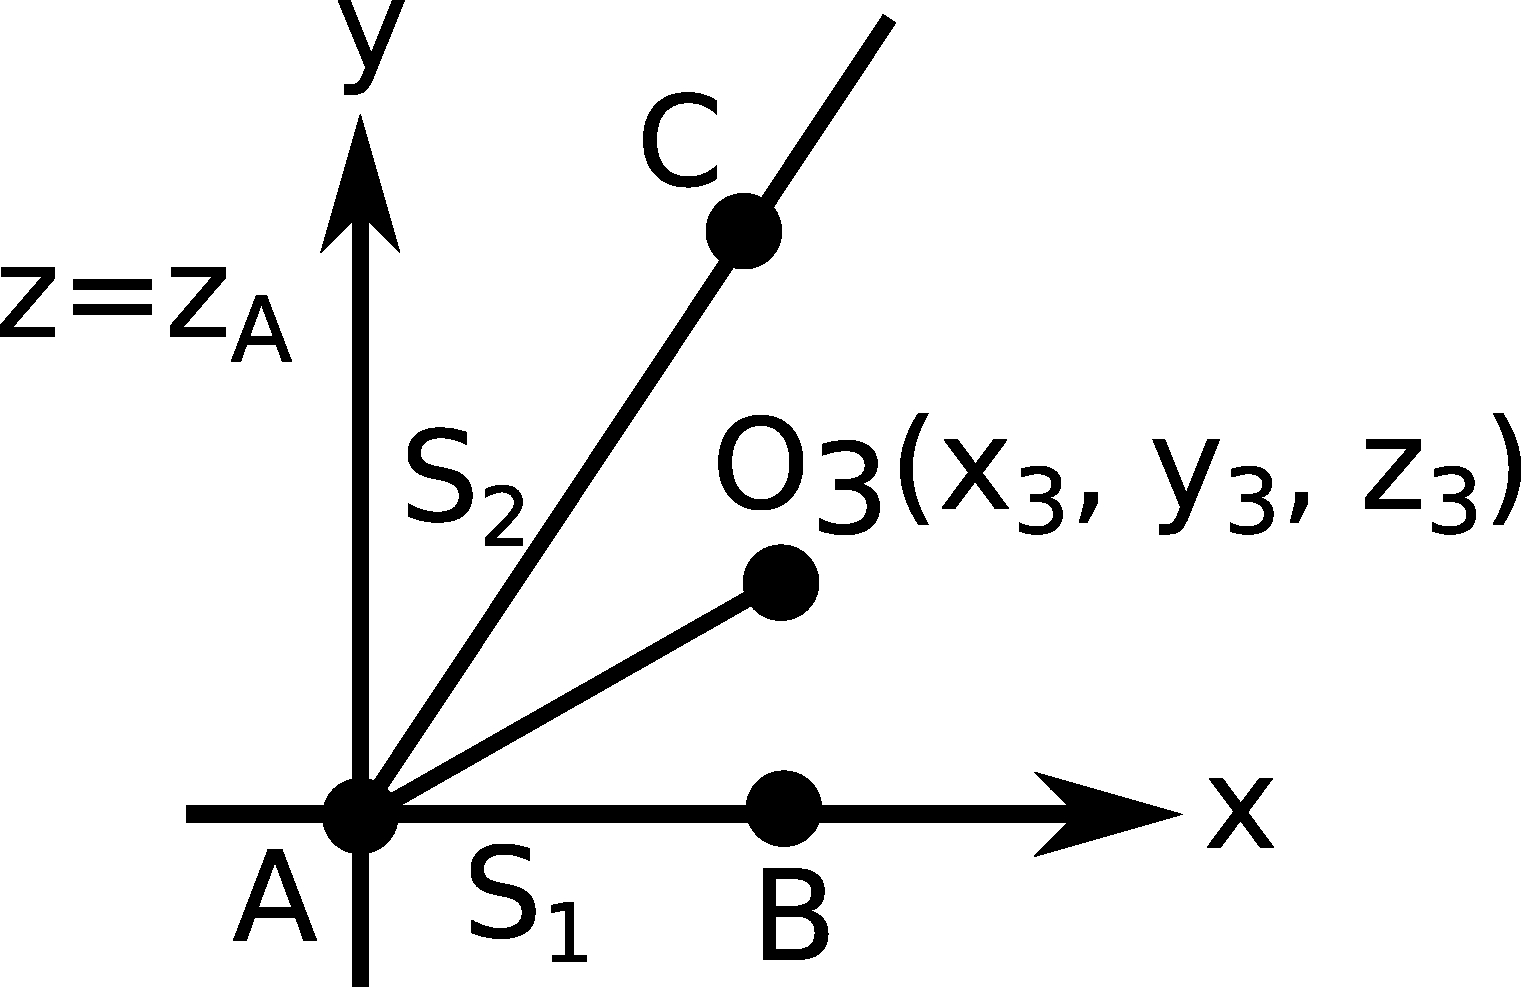
\includegraphics[width=1.5in, height=1.5in,
 keepaspectratio]{./img/HexahedraWithSphericalFaces/sectionAtVertex.jpg}
 \caption{section at $a=z_A$}
 \label{fig:sectionAtVertex}
\end{figure}

\subsection{Tetrahedron}

\begin{figure}[h!tbp]
  \begin{minipage}[t]{0.5\textwidth}
   \centering
   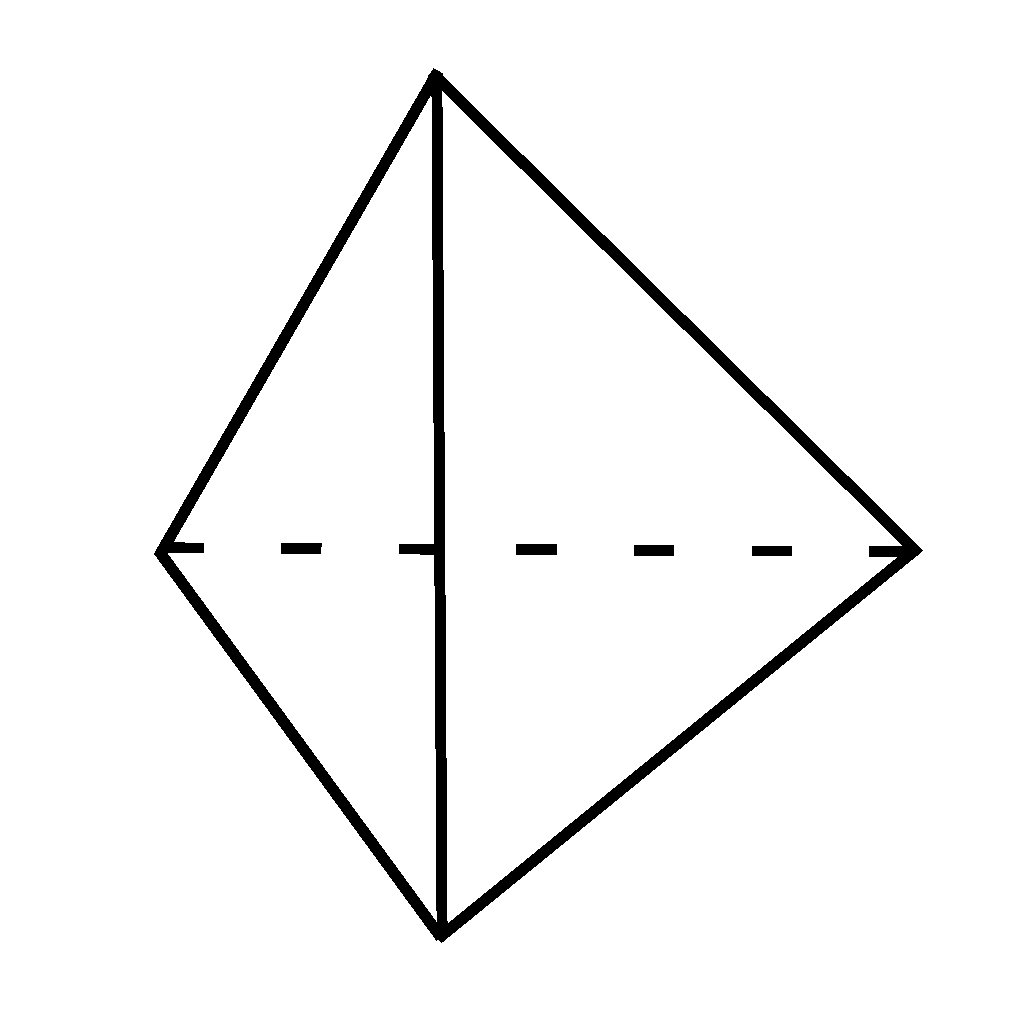
\includegraphics[width=1in, keepaspectratio]{./img/HexahedraWithSphericalFaces/tetrahedron/tetrahedron.jpg}
   \caption{Tetrahedral pyramid}
   \label{}
  \end{minipage}
 \hspace*{\fill}
  \begin{minipage}[t]{0.5\textwidth}
   \centering
   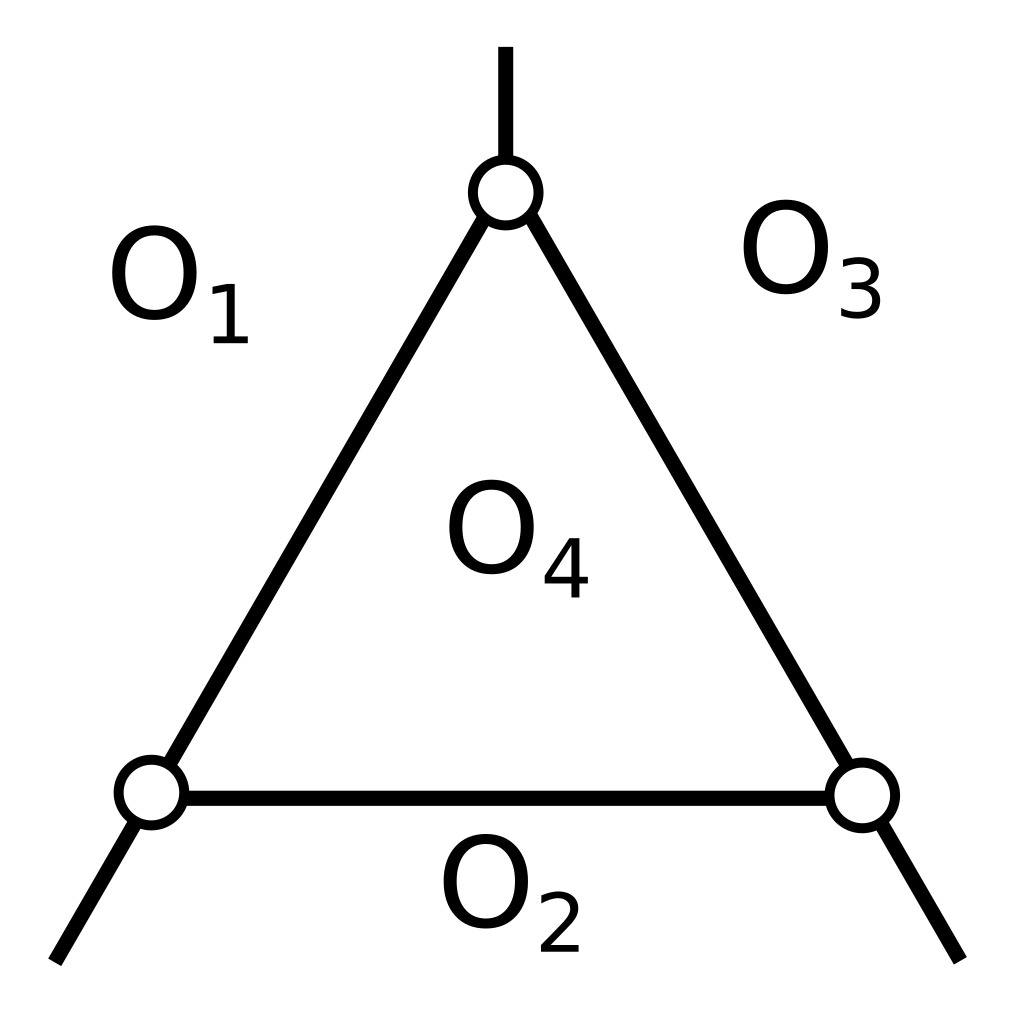
\includegraphics[width=1in, keepaspectratio]{./img/HexahedraWithSphericalFaces/tetrahedron/faces.jpg}
   \caption{Graph}
   \label{fig:tetrahedronFaces}
  \end{minipage}
 \hspace*{\fill}
\end{figure}

\begin{figure}[h!tbp]
  \begin{minipage}[t]{0.23\textwidth}
   \centering
   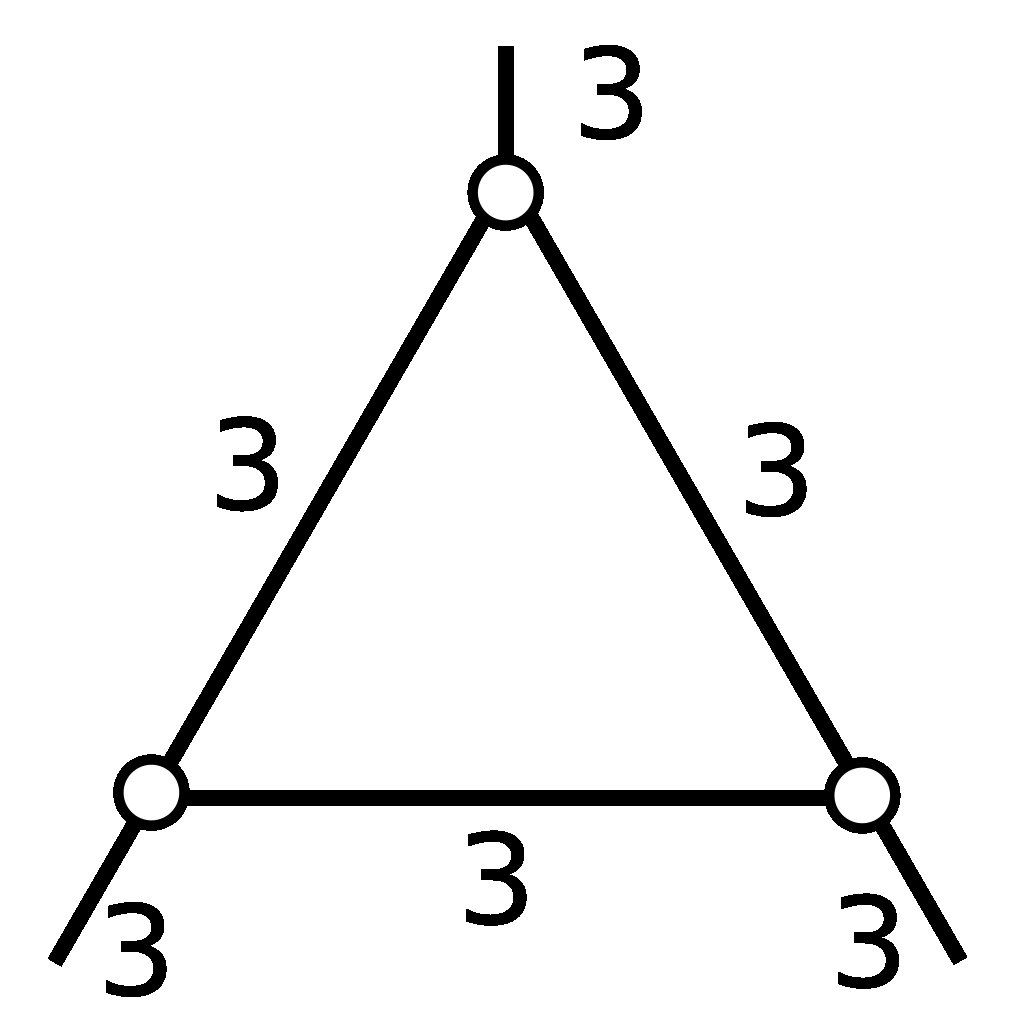
\includegraphics[width=1in,
   keepaspectratio]{./img/HexahedraWithSphericalFaces/tetrahedron/a.jpg}
   \subcaption{}
   \label{fig:}
  \end{minipage}
  \hspace*{\fill}
  \begin{minipage}[t]{0.23\textwidth}
   \centering
   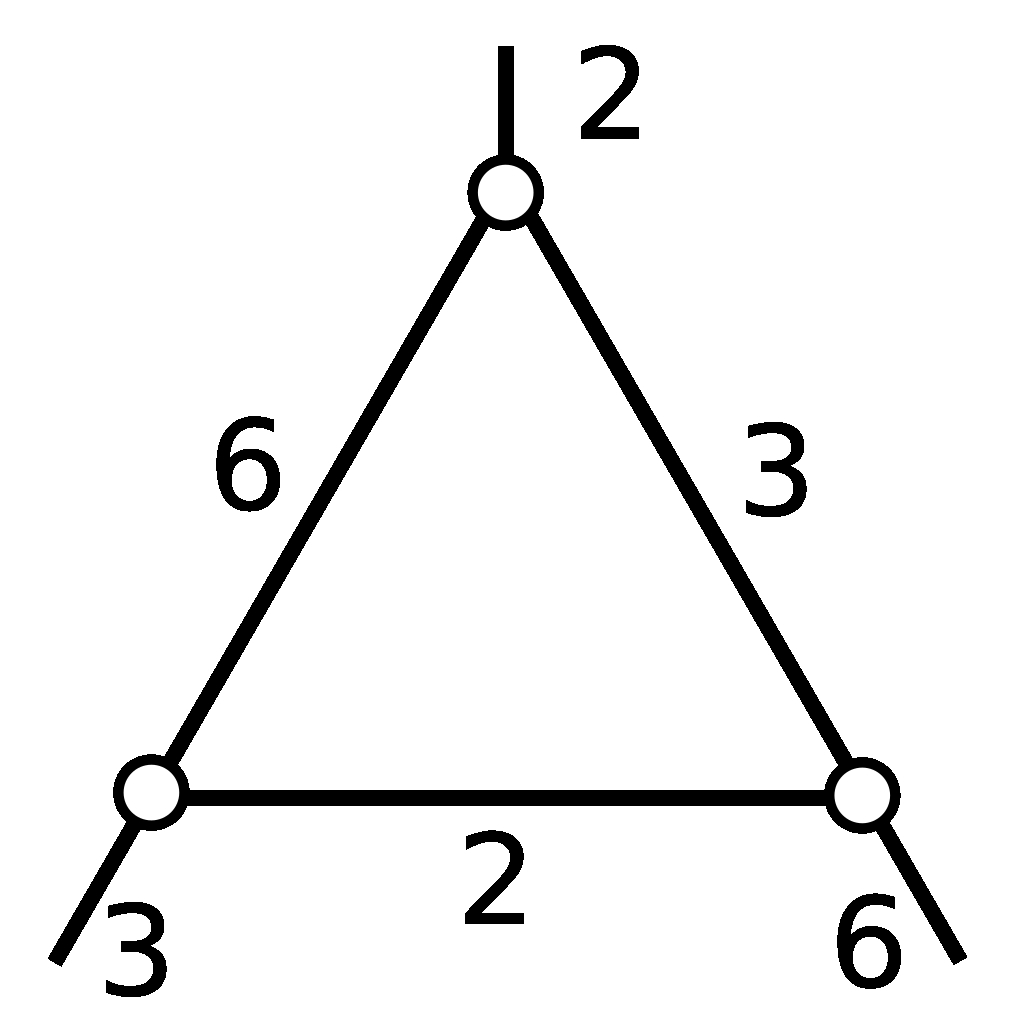
\includegraphics[width=1in, keepaspectratio]{./img/HexahedraWithSphericalFaces/tetrahedron/b.jpg}
   \subcaption{}
   \label{}
  \end{minipage}
 \hspace*{\fill}
  \begin{minipage}[t]{0.23\textwidth}
   \centering
   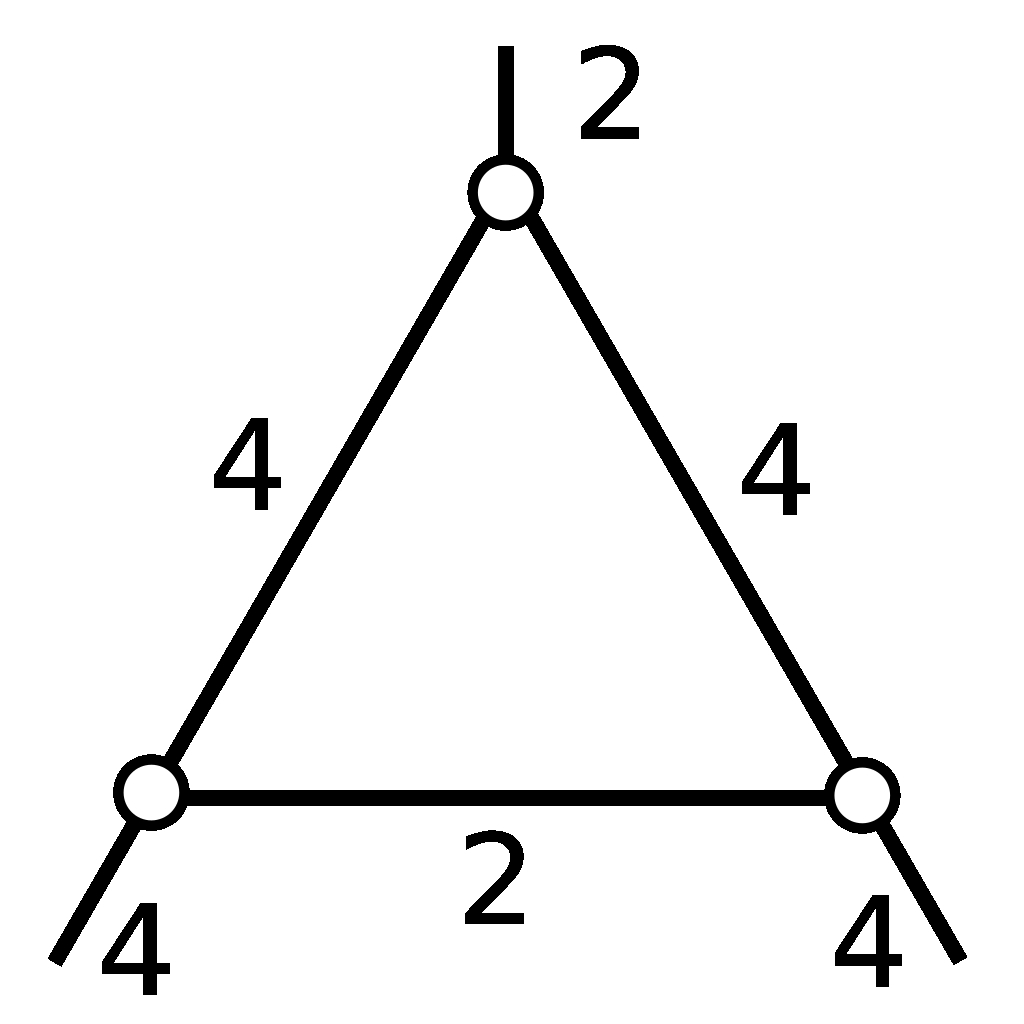
\includegraphics[width=1in, keepaspectratio]{./img/HexahedraWithSphericalFaces/tetrahedron/c.jpg}
   \subcaption{}
   \label{fig:}
  \end{minipage}
 \hspace*{\fill}
 \caption{\textit{The graph of the tetrahedron type sphairahedron}}
 \label{fig:tetrahedronCombinations}
\end{figure}

\begin{figure}[H]
 \begin{minipage}{0.5\textwidth}
  \begin{minipage}[t]{0.24\textwidth}
   \centering
   
\includegraphics[width=1.35in, height=1.35in, keepaspectratio]{./img/sphairahedron/tetrahedron/sphairahedronFinite.jpg}
   \subcaption{\textit{Sphairahedron}}
  \end{minipage}
  \hspace*{\fill}
  \begin{minipage}[t]{0.24\textwidth}
   \centering
   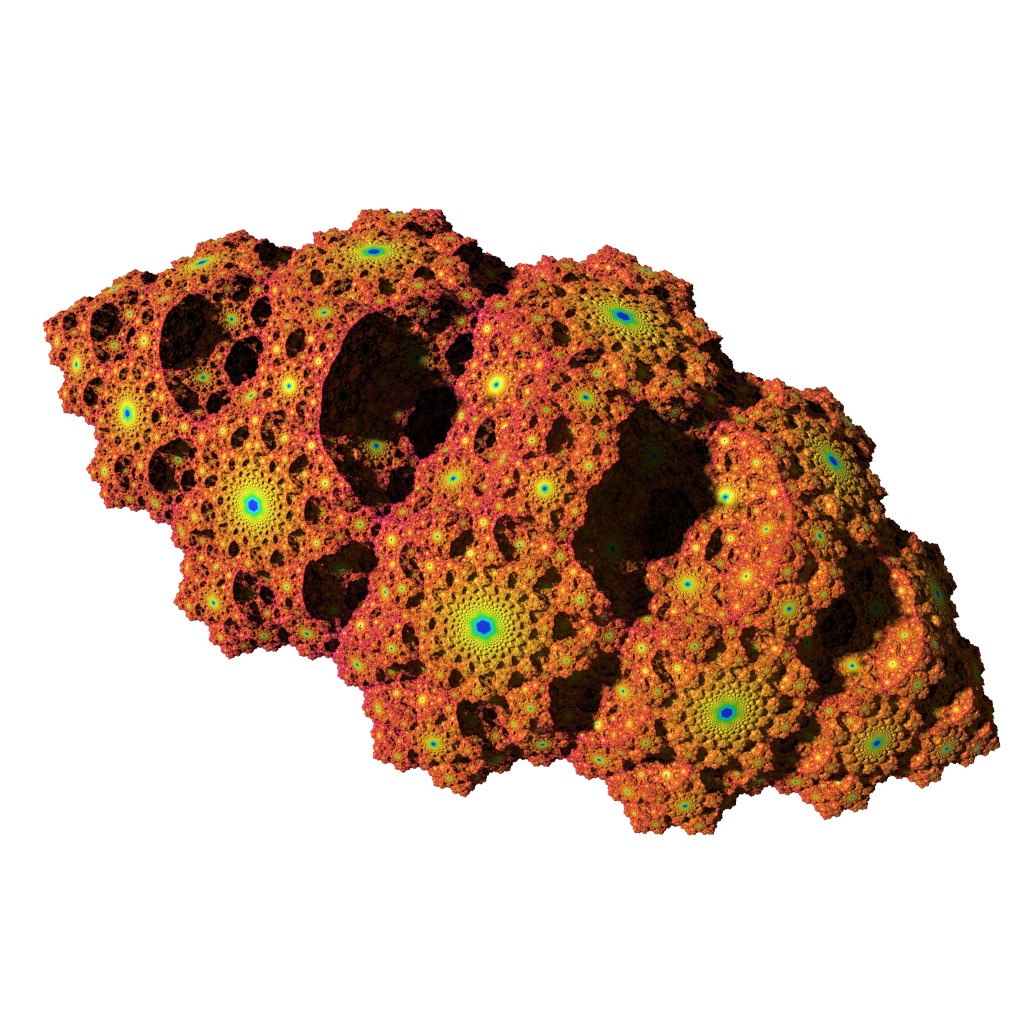
\includegraphics[width=1.35in, height=1.35in, keepaspectratio]{./img/sphairahedron/tetrahedron/limitsetFinite.jpg}
   \subcaption{\textit{Limit set}}
  \end{minipage}
  \hspace*{\fill}
  \caption{\textit{Finite tetrahedron type(a).}}
  \label{fig:tetrahedronFinite}
 \end{minipage}
 \hspace*{\fill}
 \begin{minipage}{0.5\textwidth}
  \begin{minipage}[t]{0.24\textwidth}
   \centering
   
\includegraphics[width=1.35in, height=1.35in, keepaspectratio]{./img/sphairahedron/tetrahedron/sphairahedronInf.jpg}
   \subcaption{\textit{Sphairahedron}}
  \end{minipage}
  \hspace*{\fill}
  \begin{minipage}[t]{0.24\textwidth}
   \centering
   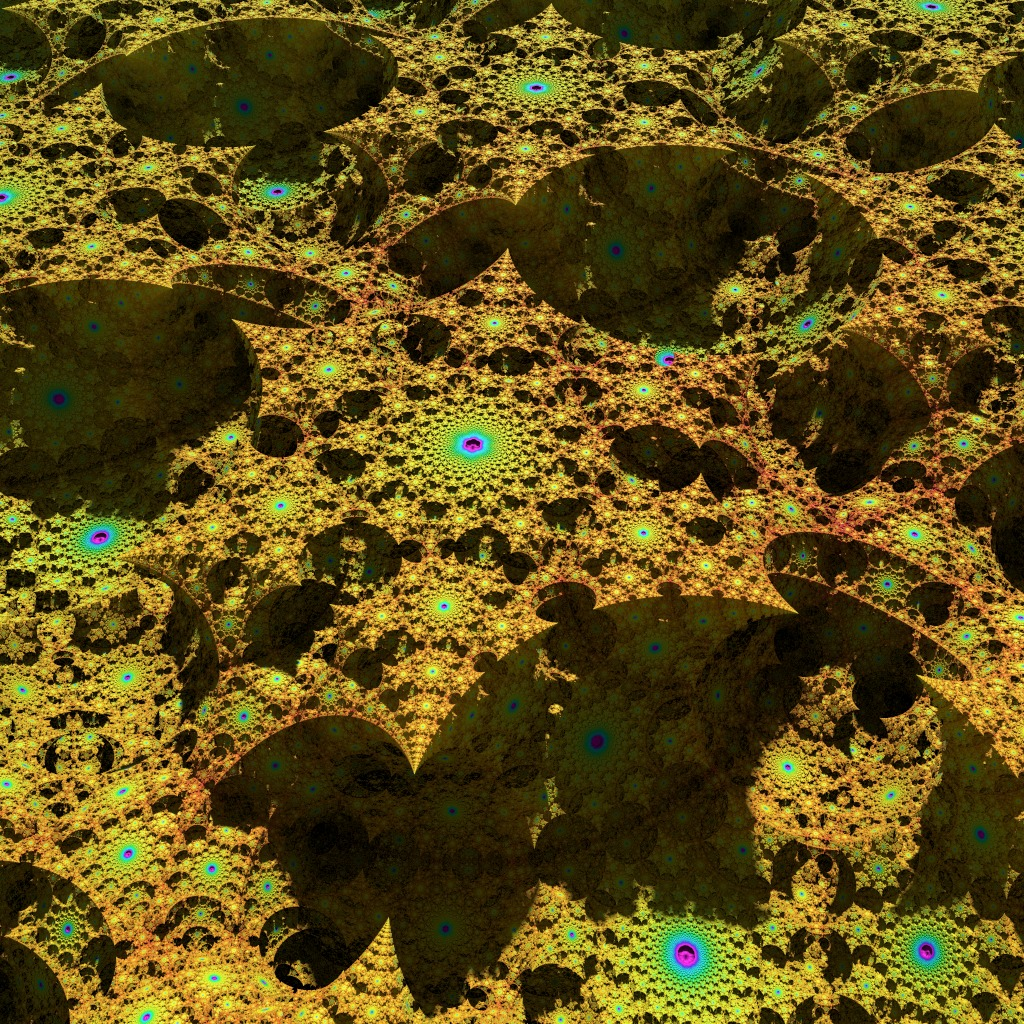
\includegraphics[width=1.35in, height=1.35in, keepaspectratio]{./img/sphairahedron/tetrahedron/limitsetInf.jpg}
   \subcaption{\textit{Limit set}}
  \end{minipage}
  \hspace*{\fill}
  \caption{\textit{Infinite tetrahedron type(a).}}
  \label{fig:tetrahedronInf}
 \end{minipage}
\end{figure}

\begin{figure}[H]
 \begin{minipage}{0.5\textwidth}
  \begin{minipage}[t]{0.24\textwidth}
   \centering
   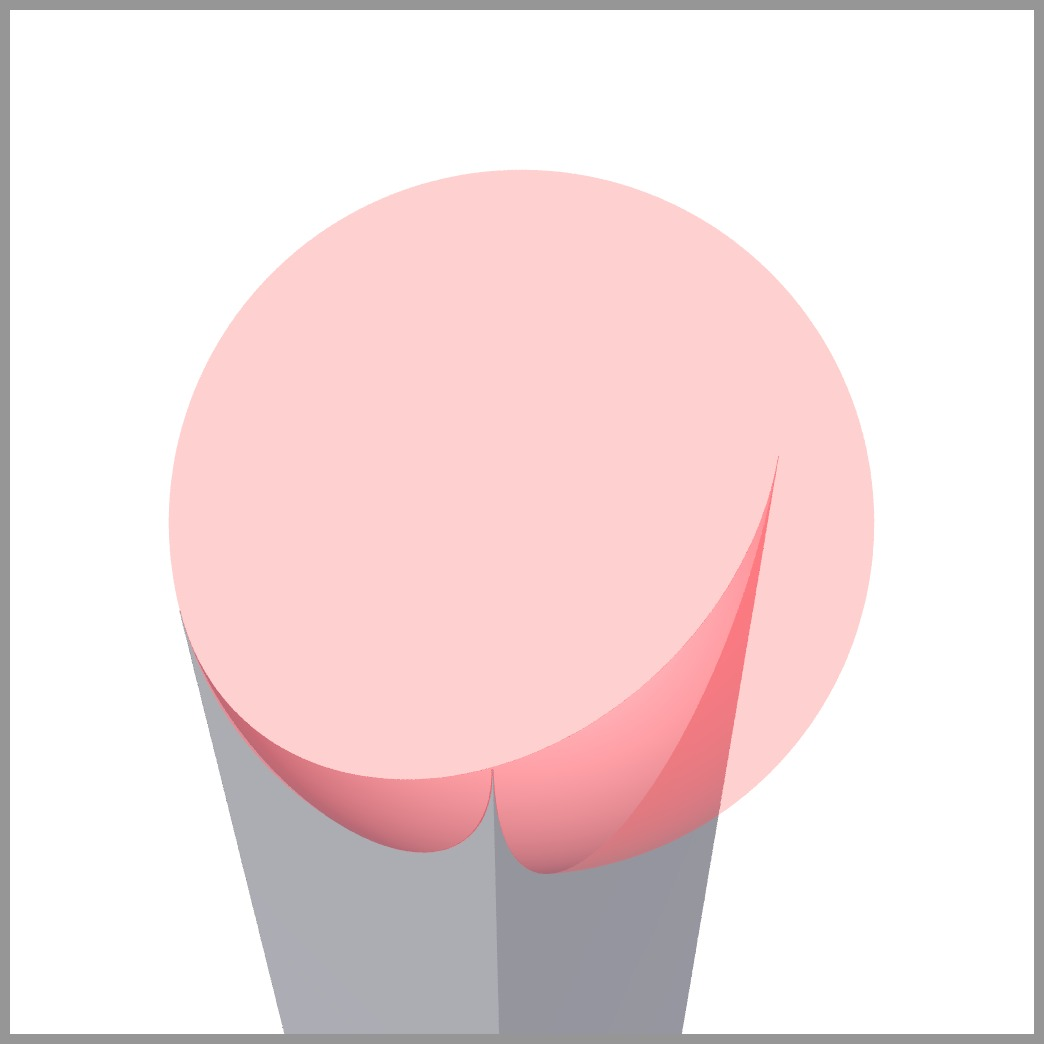
\includegraphics[width=1.35in, height=1.35in, keepaspectratio]{./img/sphairahedron/tetrahedron/sphairahedralPrism_b.jpg}
   \subcaption{\textit{Sphairahedron}}
  \end{minipage}
  \hspace*{\fill}
  \begin{minipage}[t]{0.24\textwidth}
   \centering
   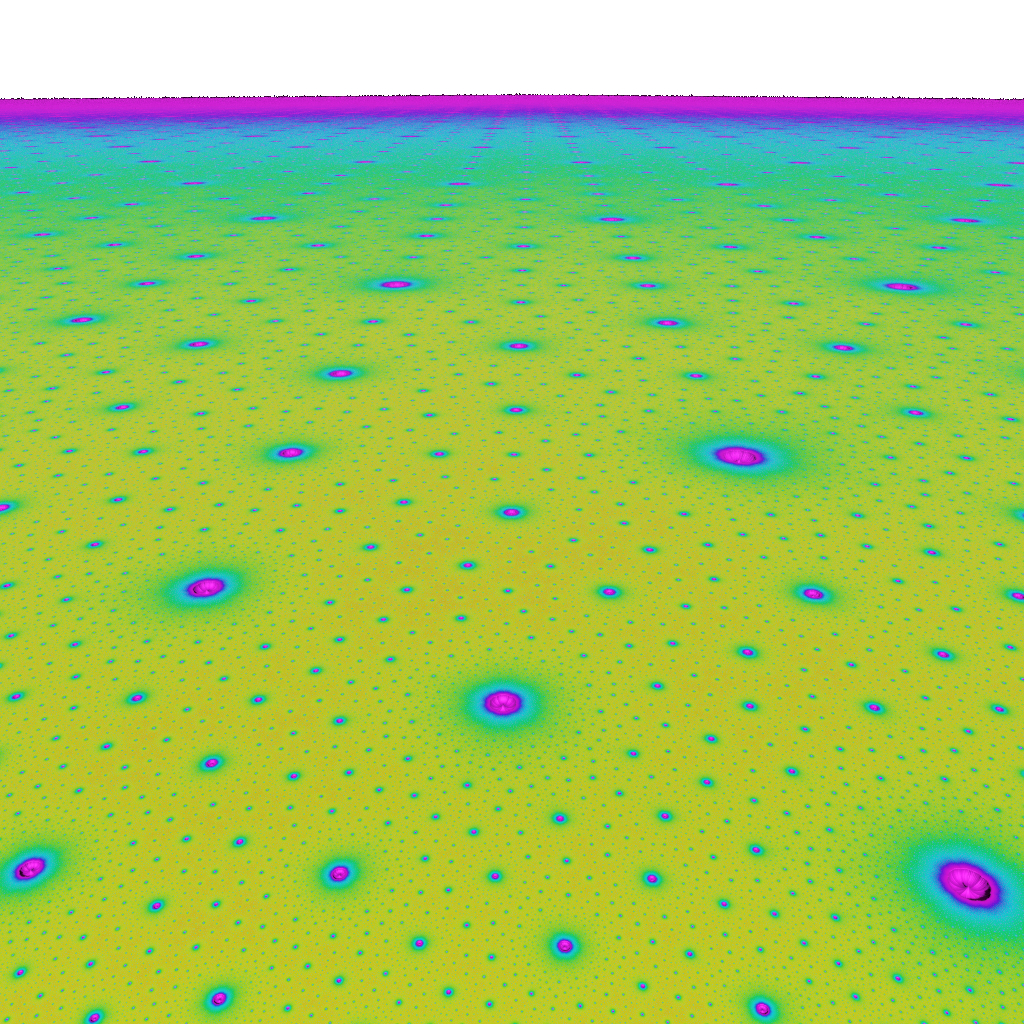
\includegraphics[width=1.35in, height=1.35in, keepaspectratio]{./img/sphairahedron/tetrahedron/limitset_b.jpg}
   \subcaption{\textit{Limit set}}
  \end{minipage}
  \hspace*{\fill}
  \caption{\textit{Infinite tetrahedron type(b).}}
  \label{fig:tetrahedronInf_b}
 \end{minipage}
 \hspace*{\fill}
 \begin{minipage}{0.5\textwidth}
  \begin{minipage}[t]{0.24\textwidth}
   \centering
   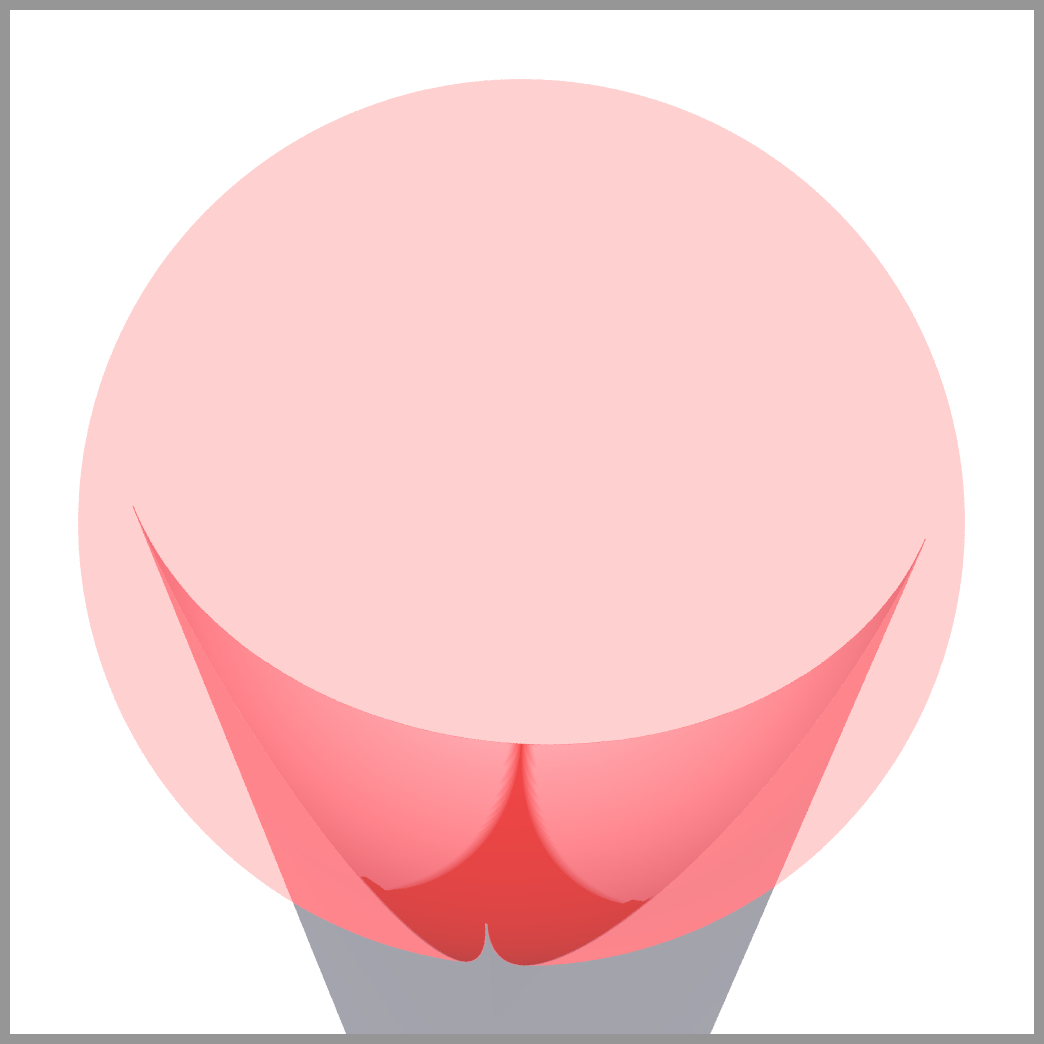
\includegraphics[width=1.35in, height=1.35in, keepaspectratio]{./img/sphairahedron/tetrahedron/sphairahedralPrism_c.jpg}
   \subcaption{\textit{Sphairahedron}}
  \end{minipage}
  \hspace*{\fill}
  \begin{minipage}[t]{0.24\textwidth}
   \centering
   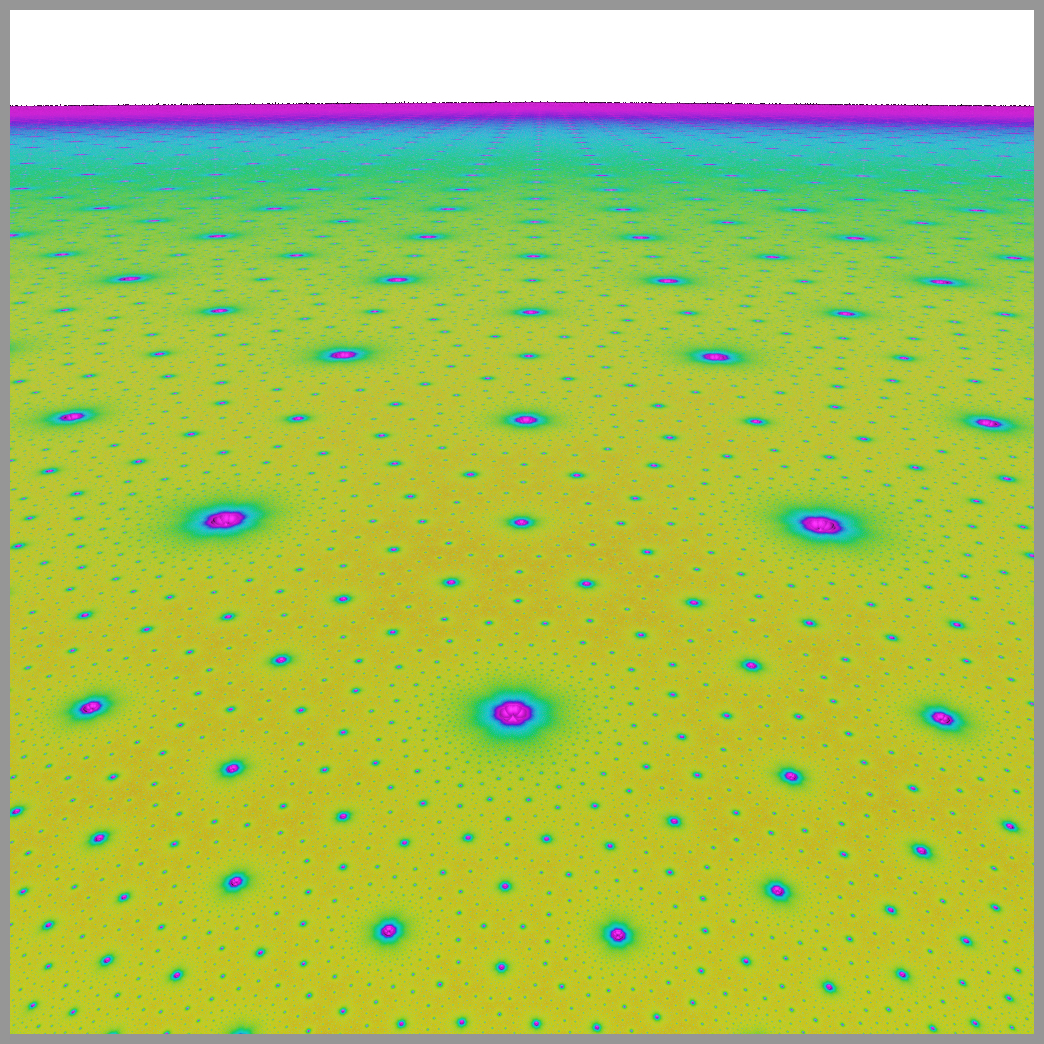
\includegraphics[width=1.35in, height=1.35in, keepaspectratio]{./img/sphairahedron/tetrahedron/limitset_c.jpg}
   \subcaption{\textit{Limit set}}
  \end{minipage}
  \hspace*{\fill}
  \caption{\textit{Infinite tetrahedron type(c).}}
  \label{fig:tetrahedronInf_c}
 \end{minipage}
\end{figure}

The tetrahedron has the fewest number of faces.
It has three types of combinations of vertexes and edges, as shown in
Figure \ref{fig:tetrahedronFaces} and Figure \ref{fig:tetrahedronCombinations}.
They have no parameter.
The quasi-spheres are shown in Figure \ref{fig:tetrahedronFinite}
, Figure \ref{fig:tetrahedronInf}, Figure \ref{fig:tetrahedronInf_b},
and Figure \ref{fig:tetrahedronInf_c}.
The tiling pattern of planes is different from the infinite sphairahedra.
They are sphere and plane, so the group is a fuchsian group.



\subsection{Compute cube-type sphairahedra}
In this paper, we deal with cube because it is simple, but it generates
complicated quasi-sphere.
Kageyama also calculates the parameter space of the cube-type
sphairahedron\cite{kageyama}.
We will formulate hexahedron of cube-type in $S^3 = R^2 \cup \{\infty\}$.
First, let $E$ be a set of edges if hexahedron of cube-type. That is,
$$
E = \{(1, 2), (1, 3), (1, 4), (1, 5), (2, 3), (2, 4), (2, 6), (3, 5),
(3, 6), (4, 5), (4, 6), (5, 6)\}.
$$
Next, let $V$ be a set of vertexes of a polyhedron. That is,
$$
V = \{(1, 2, 3), (1, 4, 5), (3, 5, 6), (1, 2, 4), (4, 5, 6), (2, 3, 6),
(2, 4, 6), (1, 3, 5)\}.
$$
We fix a sequence $\{n_{ij}\}_{(i,j) \in E}$ of natural numbers to
parametrize face-angles.

Under this preparation, we will consider a 6-ple($O_1$, ..., $O_6$)
satisfying the following conditions.

\begin{description}
 \item[(P1):] $O_i(i = 1, 2, ..., 6)$ is a sphere or a plane in $R^3
            \cup \{\infty\}$
 \item[(P2):] For each $(i, j) \in E,~O_i$ and $O_j$ intersect. Let
            $e_{ik}$ be the intersection and we call it an
            \textit{edge}. And the face-angle at $e_{ij}$ is
            $\theta_{ij} = \pi/n_{ij}$ ($n_{ij}$ is a natural number.)
 \item[(P3):] For each $(i, j, k) \in V,~e_{ij},~e_{jk}$ and $e_{ik}$
            are mutually tangent at one point. Let $v_{ijk}$ be 
            the point, and we call it a vertex. For simplicity of
            notation, we denote
\end{description}
\begin{eqnarray*}
A = v_{123},~B=v_{145},~C = v_{356},~D = v_{124}\\
E = v_{456},~F=v_{236},~G = v_{246},~H = v_{135}.
\end{eqnarray*}

Let $\tilde\varepsilon(n_{ij})$ be a set if all 6-ple $(O_1, ..., O_6)$
satisfying the above conditions. We call such 6-pre a polyhedron of
cube type. That is,
$$
\tilde\varepsilon(n_{ij}) = \{(O_1, ..., O_6)~|~(P1), (P2), (P3)\}
$$

If we parameterize $\tilde\varepsilon$ by coordinates of the center of
$O_i$, then it is naturally embedded in the Euclidean space. We consider
a natural topology on $\tilde\varepsilon$. The group M\"ob$(S^3)$ of all
M\"obius transformations in $S^3$ acts $\tilde\varepsilon$ in a natural way.
Let $\varepsilon(n_{ij})$ be its quotient space. That is,

$$
\varepsilon (n_{ij}) = \tilde\varepsilon(n_{ij}) / \text{M\"ob}(S^3)
$$

\noindent We call $\varepsilon(n_{ij})$ moduli of polyhedra.

\begin{figure}[h!tbp]
 \centering
 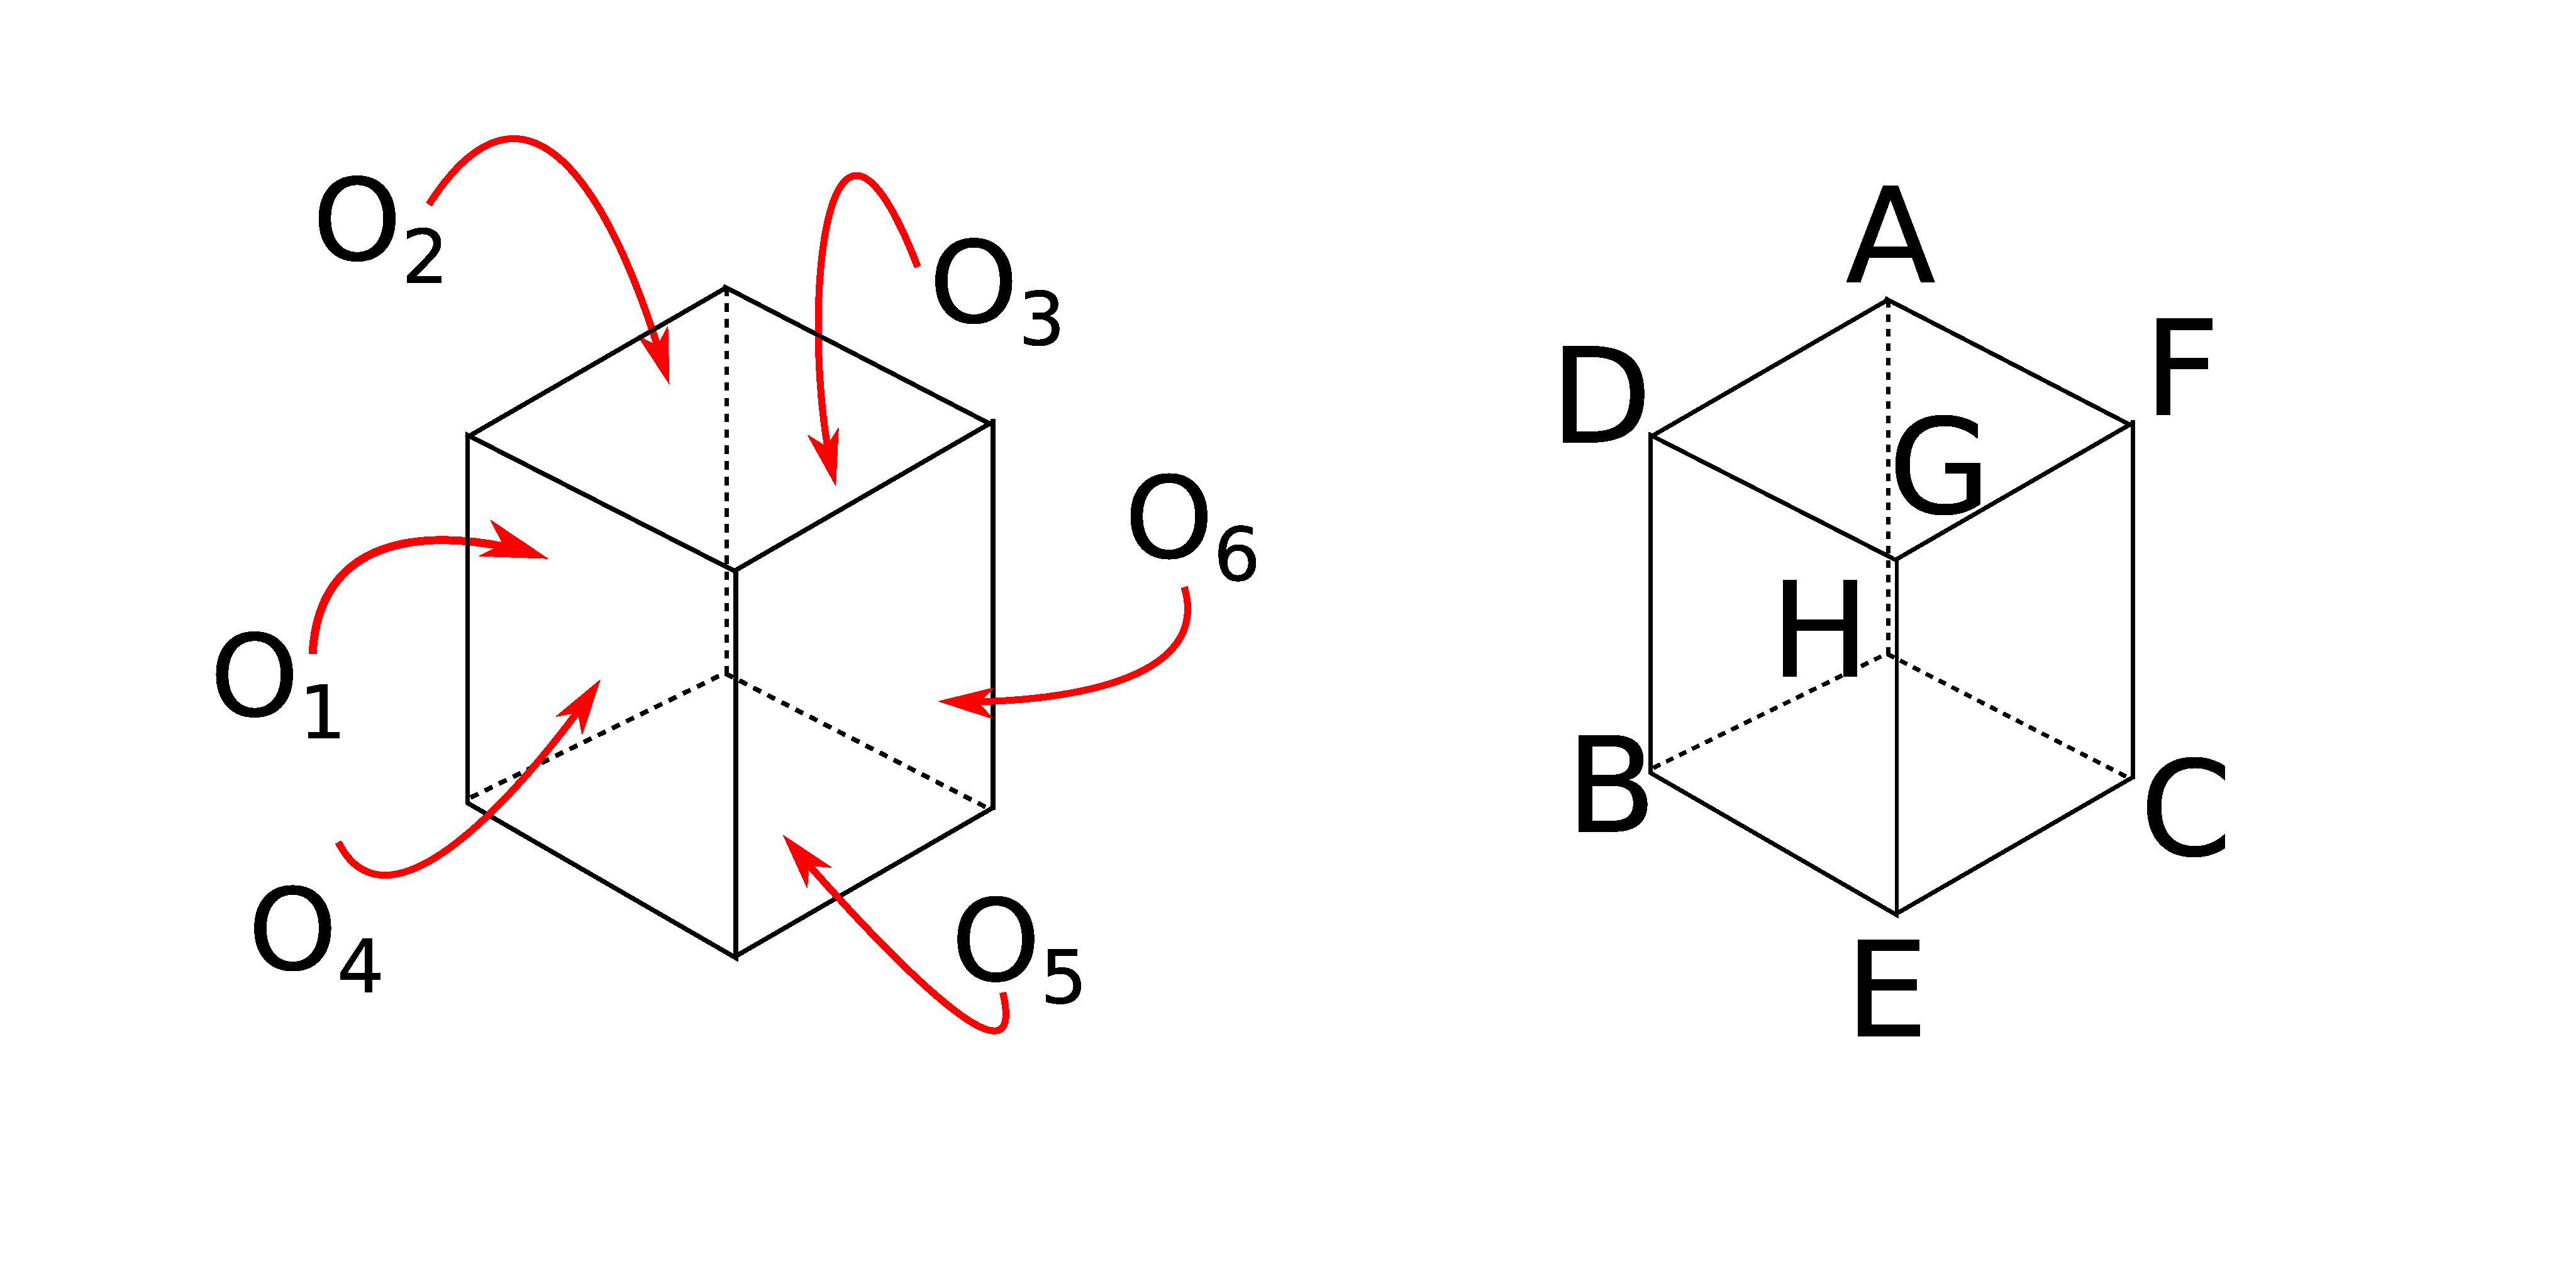
\includegraphics[width=3.5in,
 keepaspectratio]{./img/HexahedraWithSphericalFaces/cubes.jpg}
 \caption{}
 \label{fig:cubes}
\end{figure}

\begin{figure}[h!tbp]
 \begin{minipage}[t]{0.5\textwidth}
 \centering
 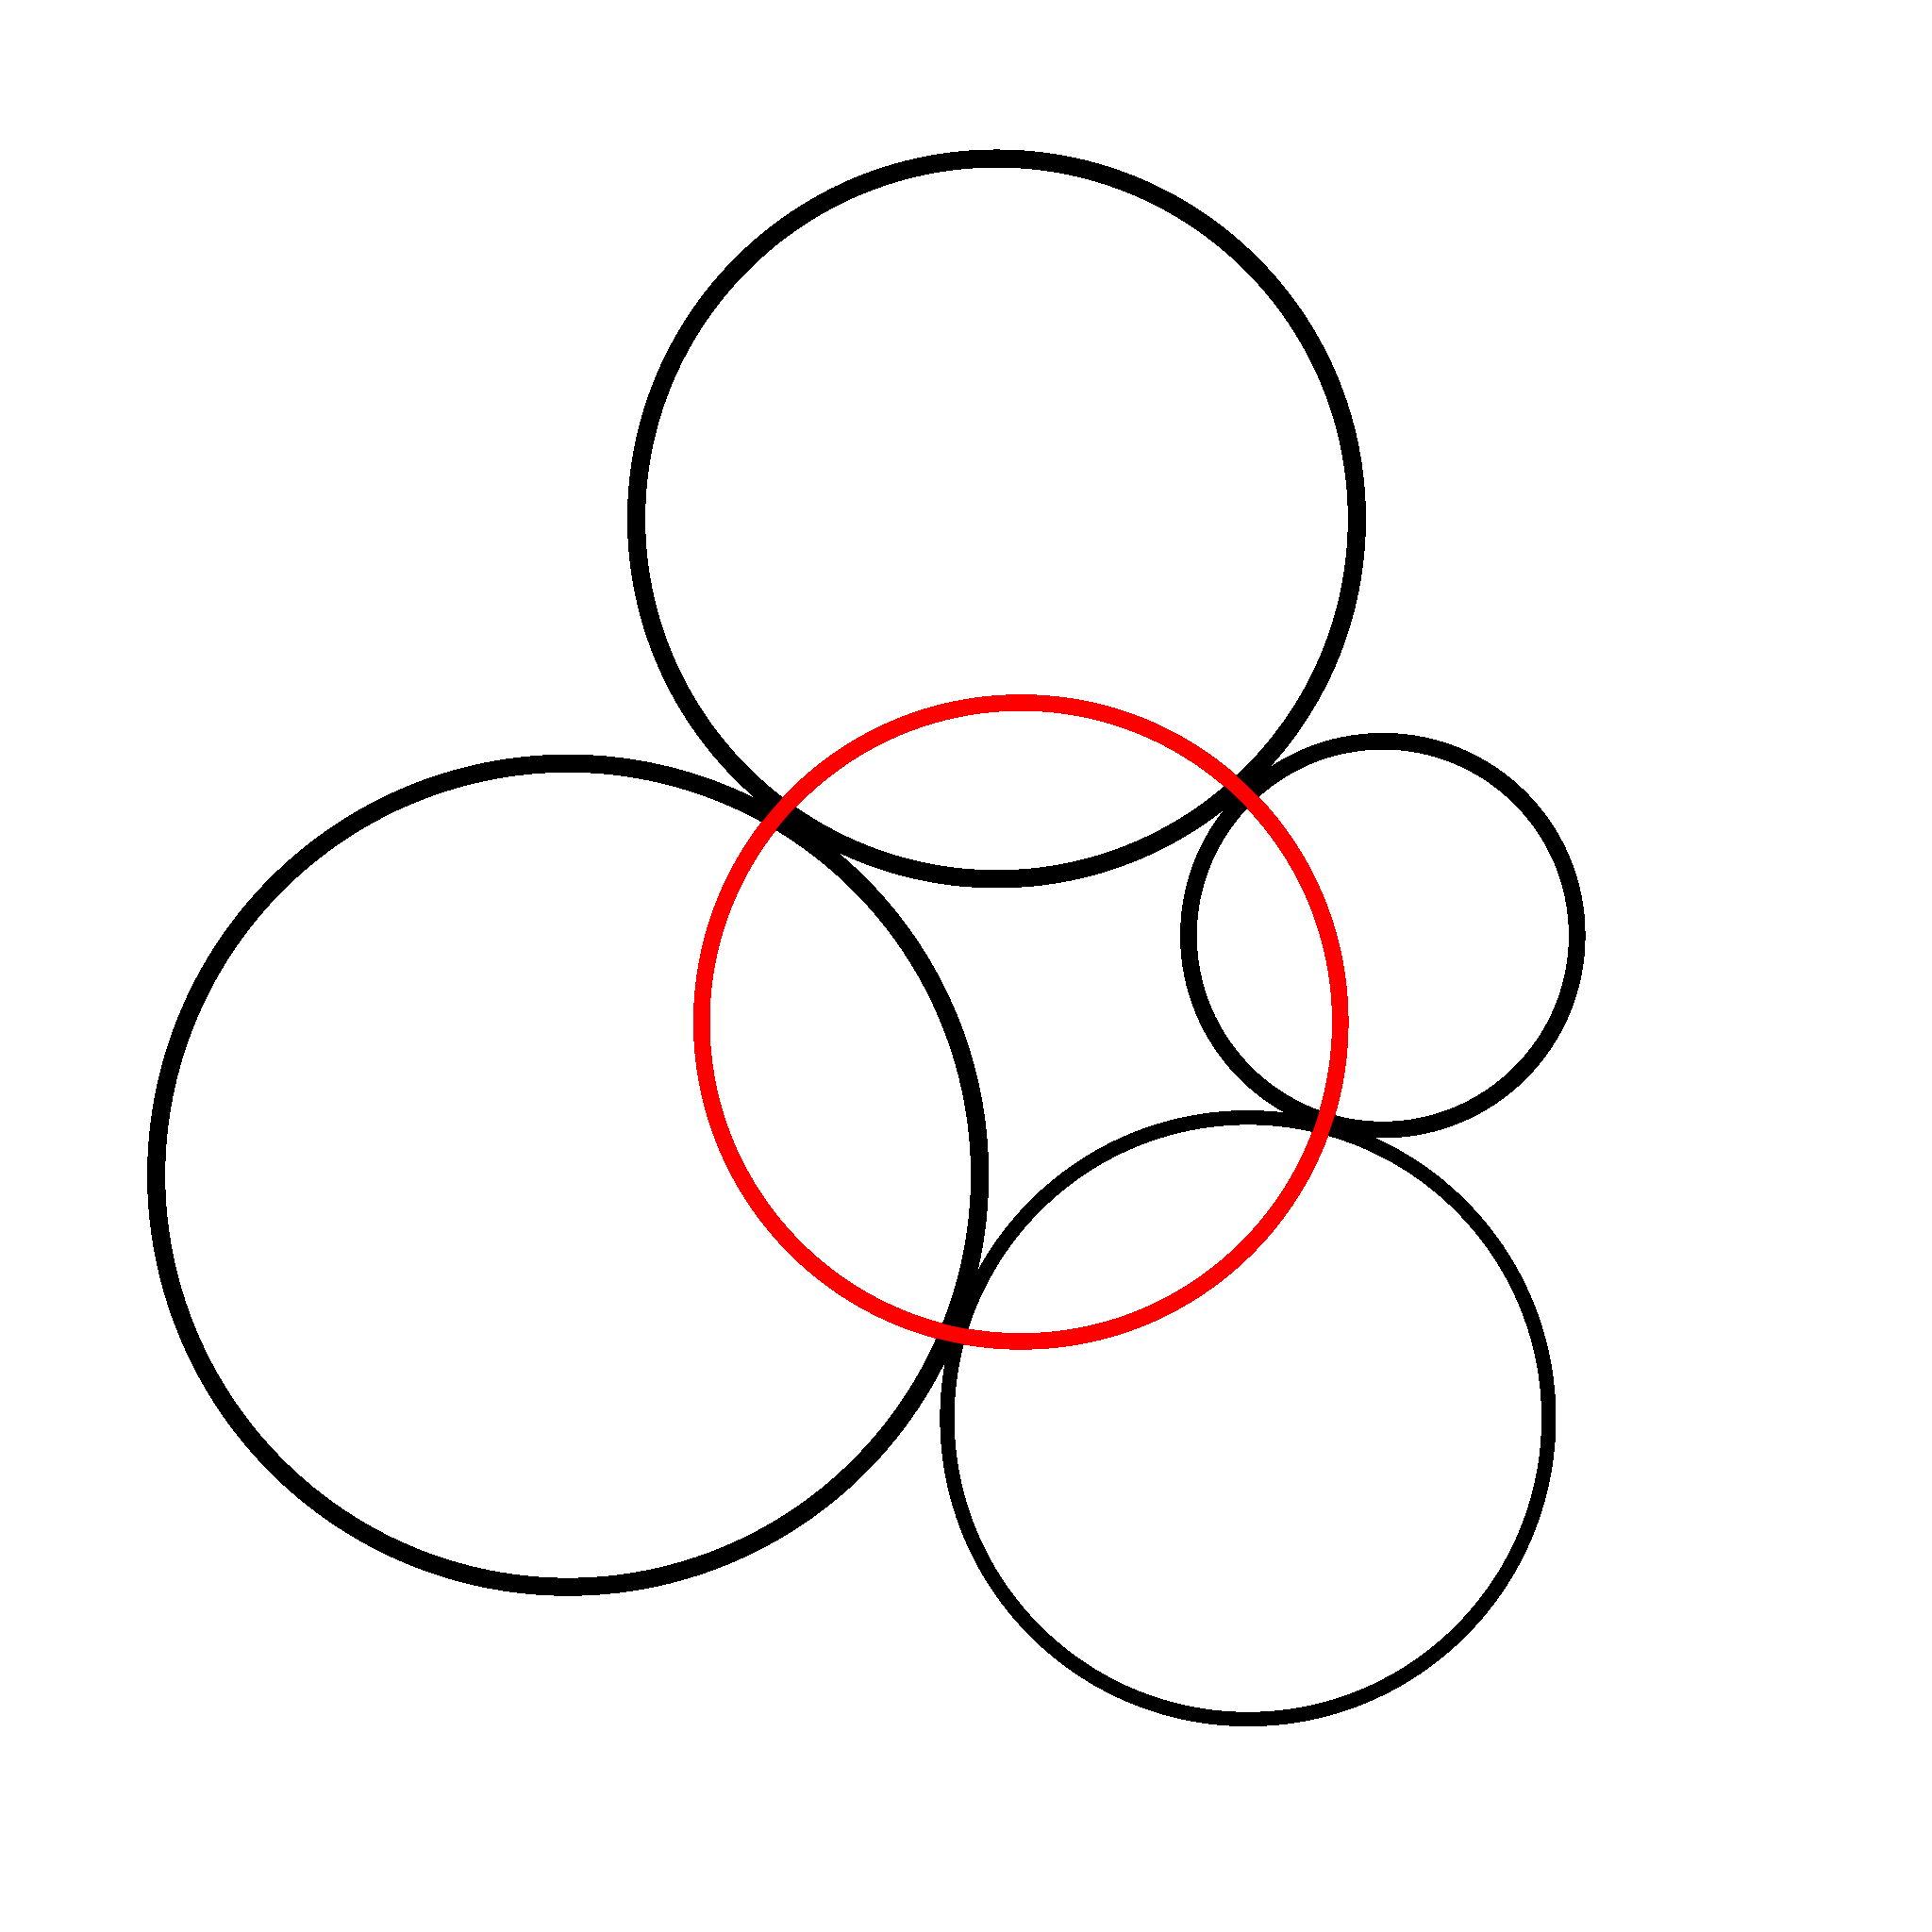
\includegraphics[width=1.5in, height=1.5in,
 keepaspectratio]{./img/HexahedraWithSphericalFaces/chain.jpg}
 \caption{}
 \label{fig:chainCircles}
 \end{minipage}
 \hspace*{\fill}
 \begin{minipage}[t]{0.5\textwidth}
  \centering
  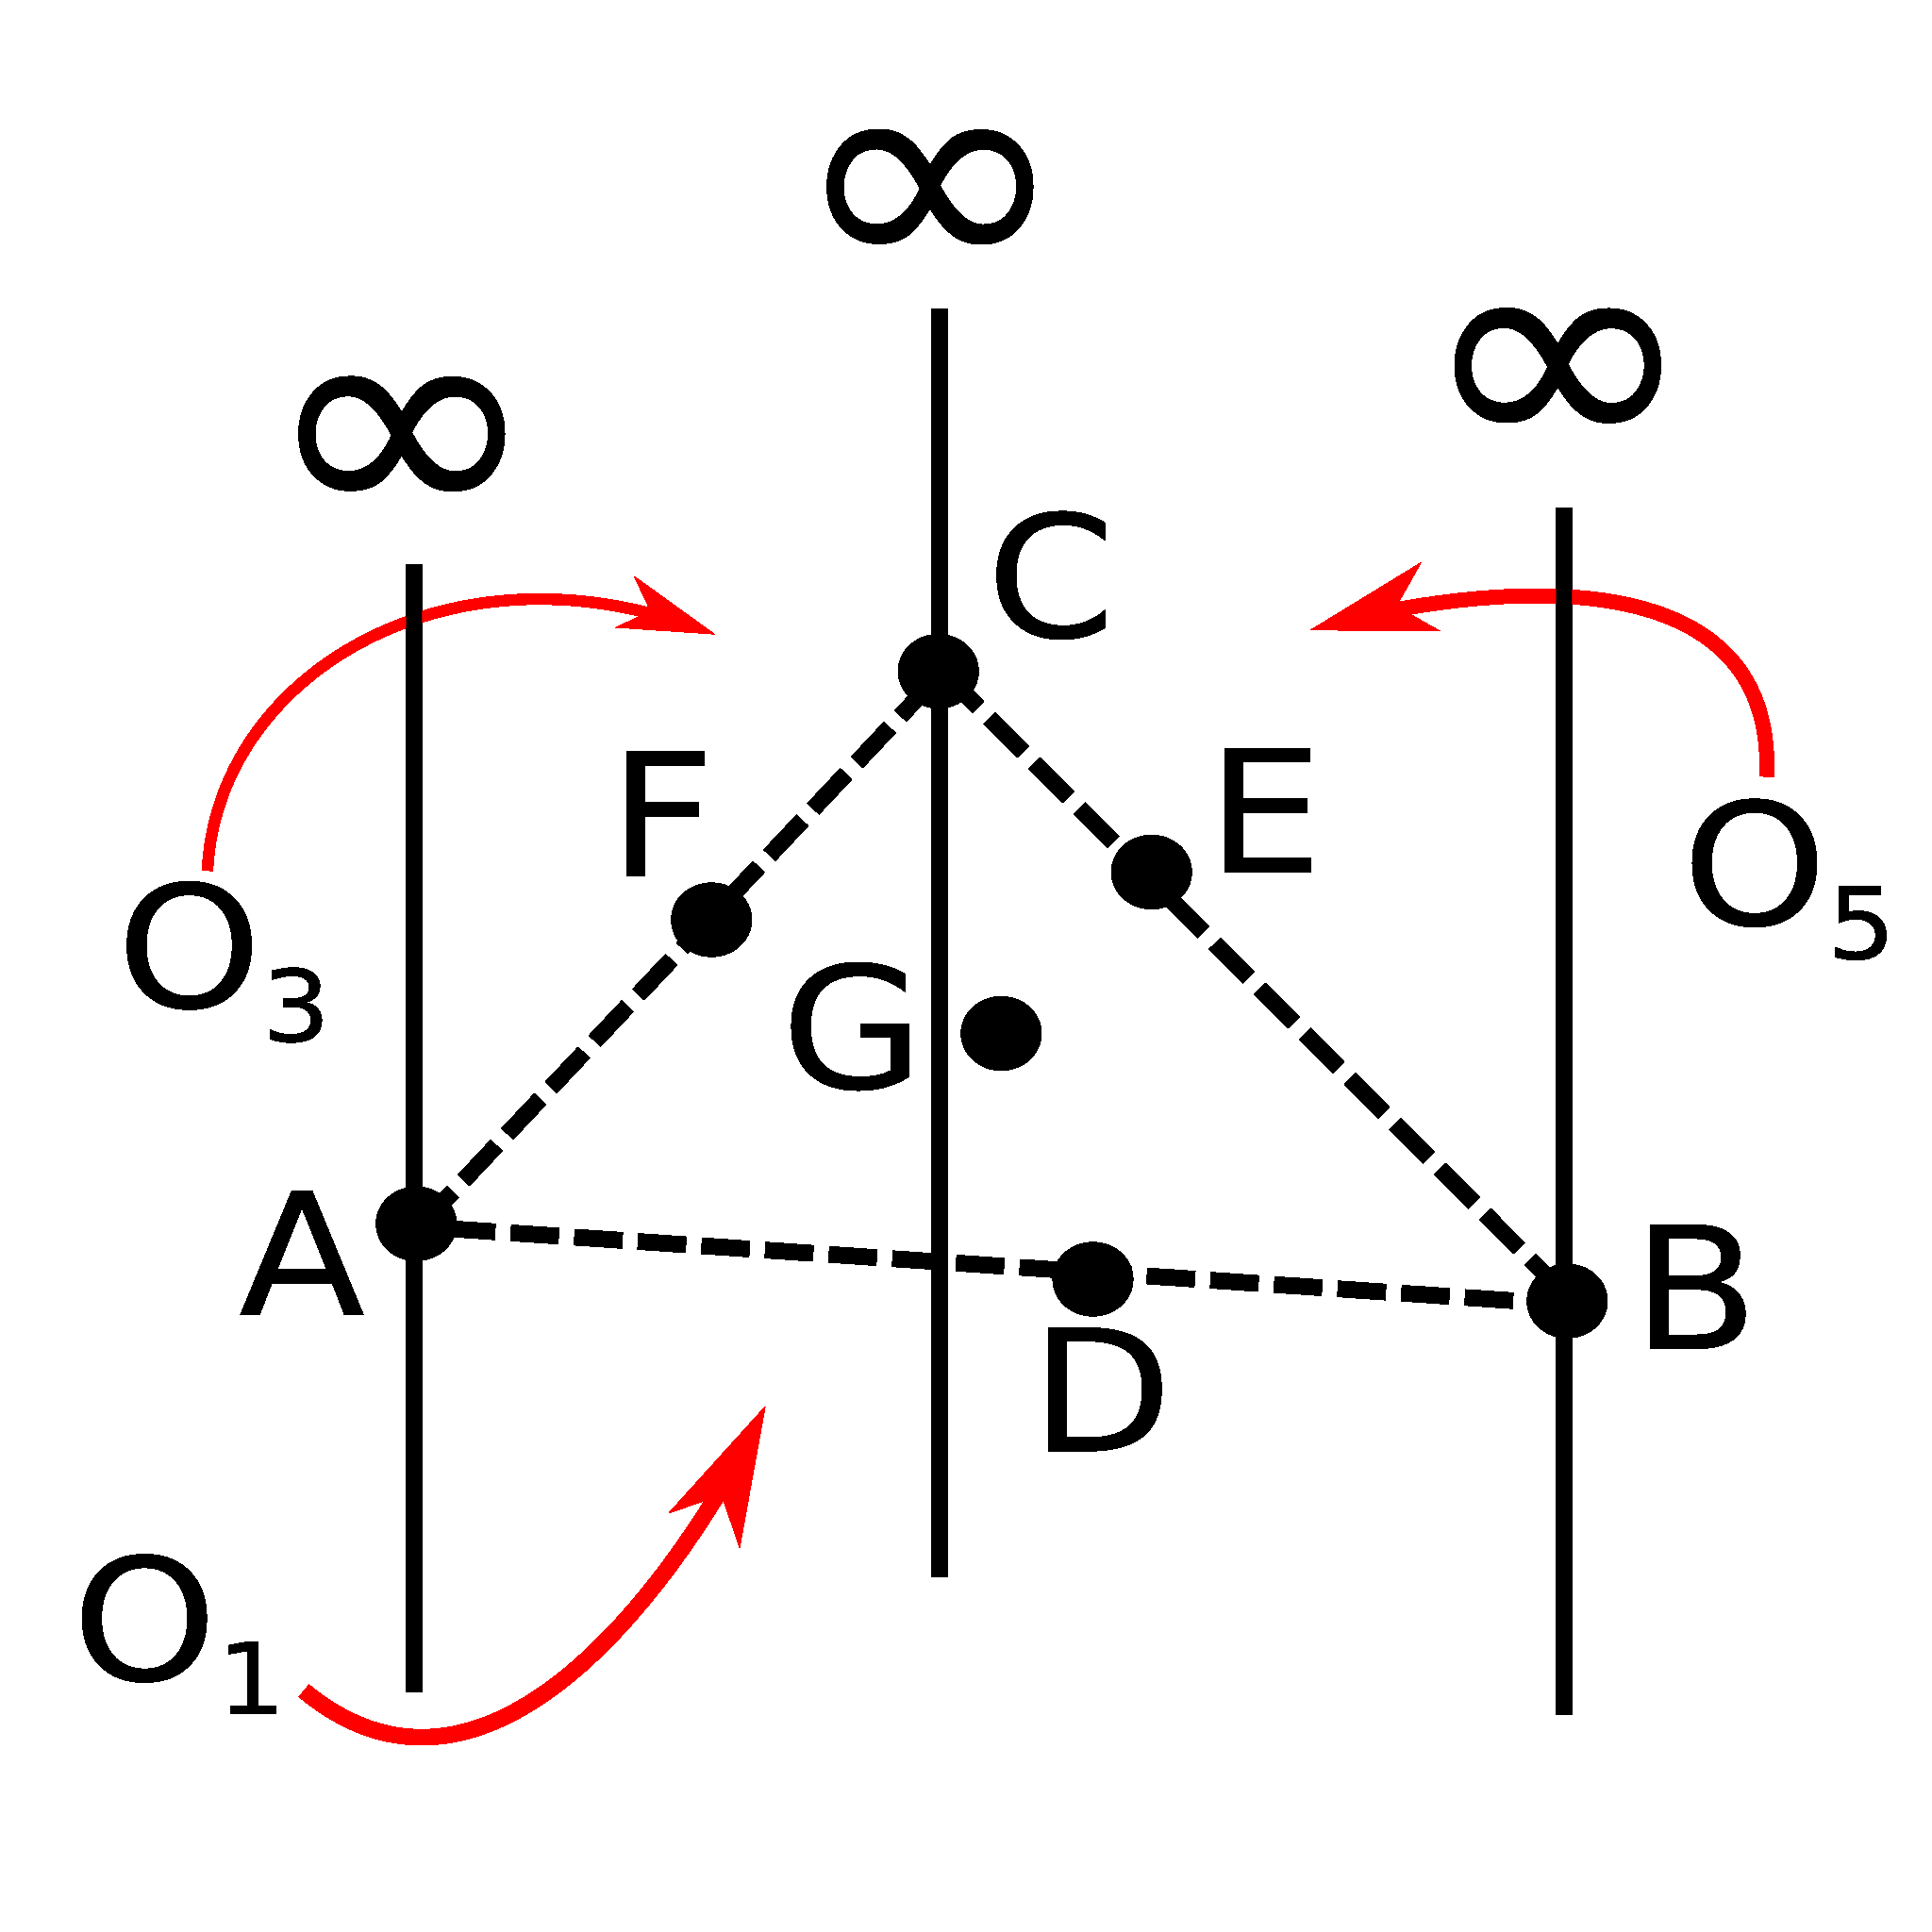
\includegraphics[width=1.5in, height=1.5in,
  keepaspectratio]{./img/HexahedraWithSphericalFaces/infTriangle.jpg}
  \caption{}
  \label{fig:infTriangle}
 \end{minipage}
 \hspace*{\fill}
\end{figure}

\subsection{Preparations}

We will show some lemmas in this subsection.

First of all, we define a \textit{limit ball}.
\begin{definition}
 The Limit ball is the shape whose limit set is its boundary surface,
 and we obtain it by tiling of the sphairahedron $P$.
$$
 G = G_p := \left< \text{inversion of}~ S~|~S~\text{is surface of}~P
 \right>,
 \text{Limit ball of}~P : LimitBall(P) := G_p(P)
$$
\end{definition}

\begin{lemma}\label{sameCircle}
For each $O_i$, the four vertexes on $O_i$ lie on the same circle.
Hence the four vertexes lie on one plane in $R^3$.
\end{lemma}

\begin{proof}
 We know the following famous lemma about four circles: If four circles 
 $C_1,~C_2,~C_3,~C_4$ on a plane, and they are mutually tangent like a
 chain as in Figure \ref{fig:chainCircles}, then the four tangent points lie on one circle.
 (See figure \ref{fig:chainCircles}) Using this lemma we will show lemma \ref{sameCircle} We fix $i$ and
 consider only on $O_i$. If $O_i$ is not a plane, we transform 
 ($O_1, ..., O_6$) by a M\"obius transformation such that $O_i$ is a
 plane. There are four edges on $O_i$, and they are circles and are
 mutually tangent like a chain. From the above well-known lemma. The
 four vertexes on $O_i$ lie on one circle on $O_i$. If we re-transform
 ($O_i, ..., O_6$) back, the four vertexes still lie on one circle,
 because any M\"obius transformation maps a planer circle to a planer circle.
\end{proof}

\begin{lemma}\label{eightVertexes}
 Eight vertexes of a polyhedron of cube-type lie in the same sphere.
\end{lemma}

\begin{proof}
 There is a M\"obius transformation $\phi$ such that it moves the vertex
 $H$ to the infinity point. (See Figure \ref{fig:infTriangle}.) From Lemma \ref{sameCircle}, the three
 vertexes $A, D,$ and $B$ lie on one straight line. In the same way,
 three vertexes $A, D, G,$ and $F$ lie on one planar circle, all vertexes
 except $H$ line on one plane. We transform them back by $\phi^{-1}$, and
 we get the conclusion of Lemma \ref{eightVertexes}.
\end{proof}


 Using this Lemma \ref{sum}, we obtain the following lemma in a combinatorial way.
% 12-pre or twelve-pre
\begin{lemma}\label{combination}
 12-ple($n_{ij}$) = ($n_{12}, n_{13}, n_{14}, n_{15}, n_{23}, n_{24},
 n_{26}, n_{35}, n_{36}, n_{45}, n_{46}, n_{56}$) of face-angle
 parameters is one of the following 11.(See Figire \ref{fig:cubeGraph}.)
\end{lemma}

\noindent
(a) (3, 3, 3, 3, 3, 3, 3 ,3 ,3 ,3 ,3 ,3)\\
(b) (2, 3, 3, 3, 6, 6, 2, 3, 3, 3, 3, 3)\\
(c) (2, 3, 6, 3, 6, 3, 2, 3, 3, 2, 6, 3)\\
(d) (6, 2, 3, 3, 3, 2, 3, 6, 3, 3, 6, 2)\\
(e) (3, 2, 2, 3, 6, 6, 2, 6, 3, 6, 3, 2)\\
(f) (3, 2, 2, 3, 6, 6, 3, 6, 2, 6, 2, 3)\\
(g) (6, 2, 2, 3, 3, 3, 6, 6, 2, 6, 2, 3)\\
(h) (3, 2, 6, 3, 6, 2, 3, 6, 2, 2, 6, 3)\\
(i) (4, 2, 2, 4, 4, 4, 2, 4, 4, 4, 4, 2)\\
(j) (4, 2, 2, 4, 4, 4, 4, 4, 2, 4, 2, 4)\\
(k) (6, 2, 2, 4, 3, 3, 6, 4, 2, 4, 2, 4)\\

\begin{figure}[h!tbp]
  \begin{minipage}[t]{0.15\textwidth}
   \centering
   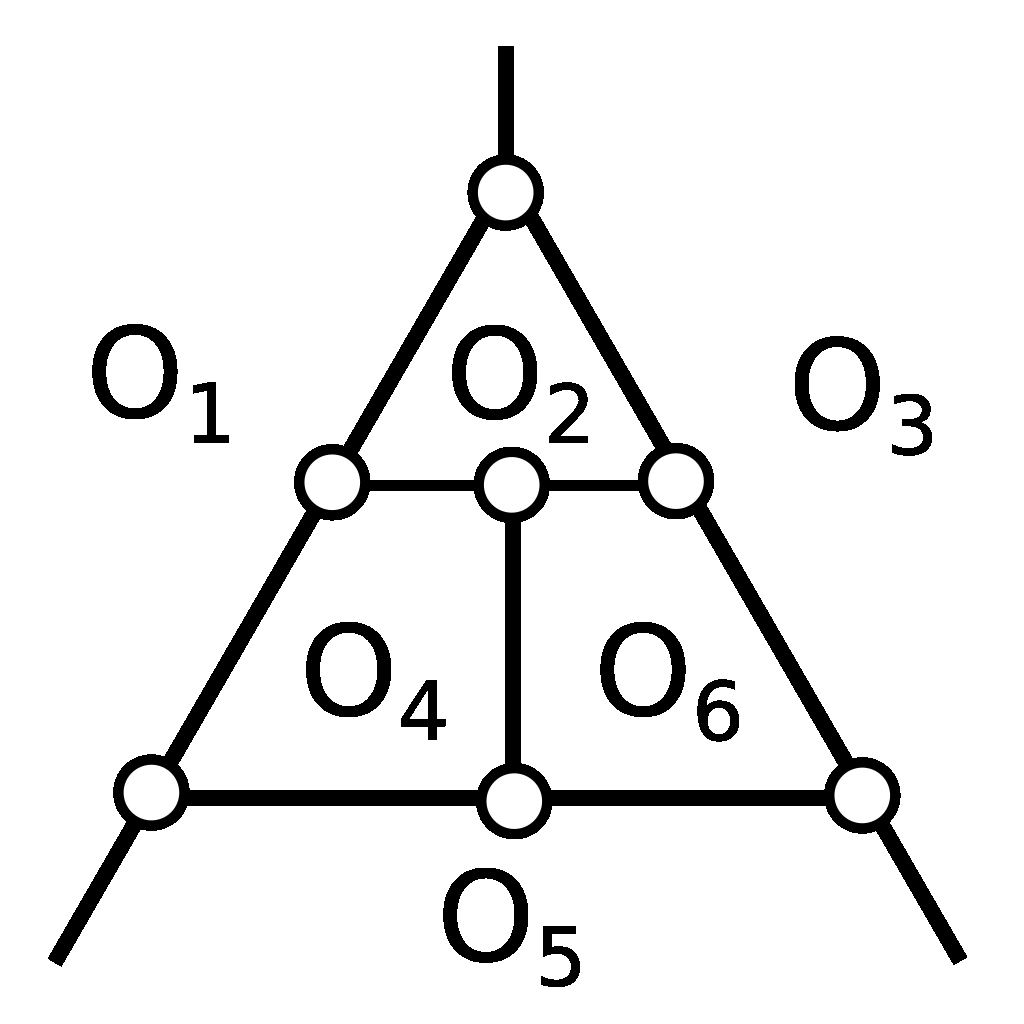
\includegraphics[width=0.8in, keepaspectratio]{./img/HexahedraWithSphericalFaces/cube/cubeFaces.jpg}
   \caption{Graph}
   \label{}
  \end{minipage}
 \hspace*{\fill}
 \begin{minipage}[t]{0.75\textwidth}
  \begin{minipage}[t]{0.15\textwidth}
   \centering
   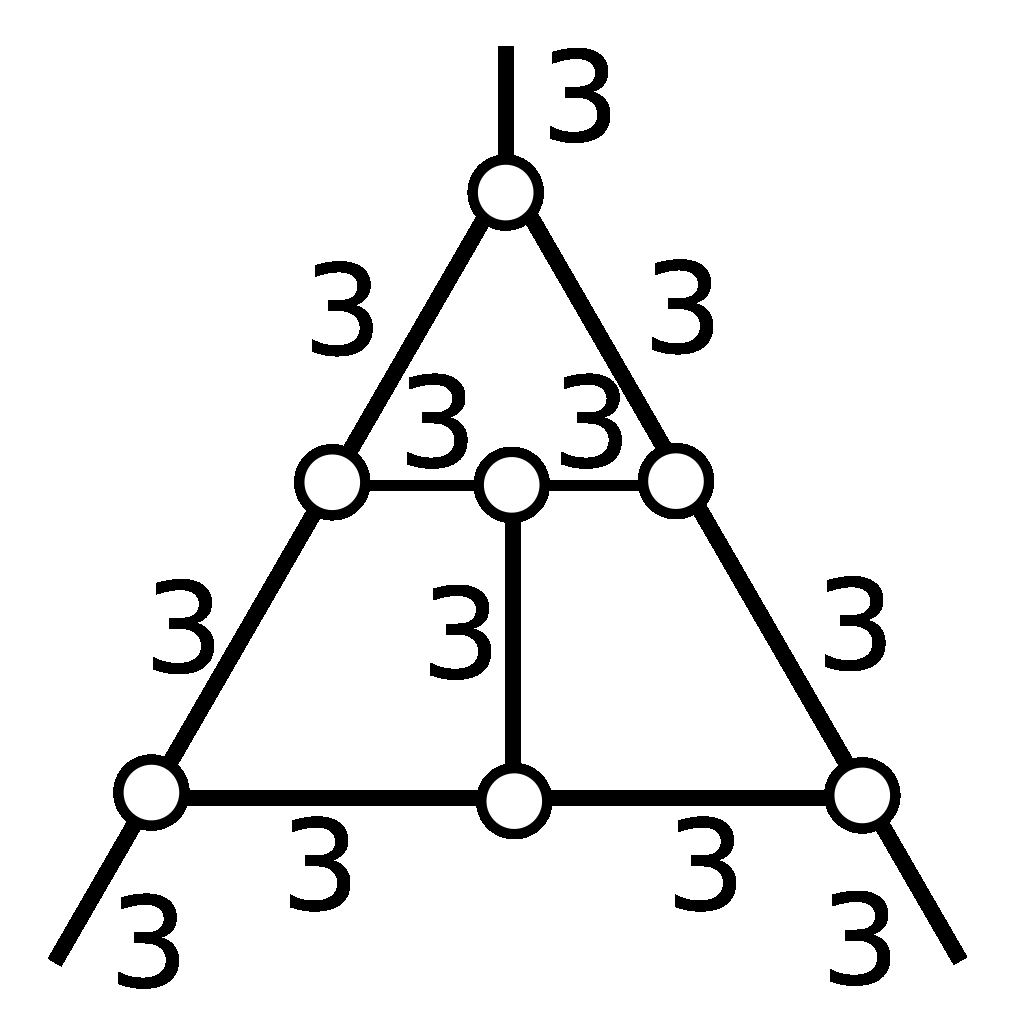
\includegraphics[width=0.8in,
   keepaspectratio]{./img/HexahedraWithSphericalFaces/cube/cube_a.jpg}
   \subcaption{}
   \label{fig:}
  \end{minipage}
  \hspace*{\fill}
  \begin{minipage}[t]{0.15\textwidth}
   \centering
   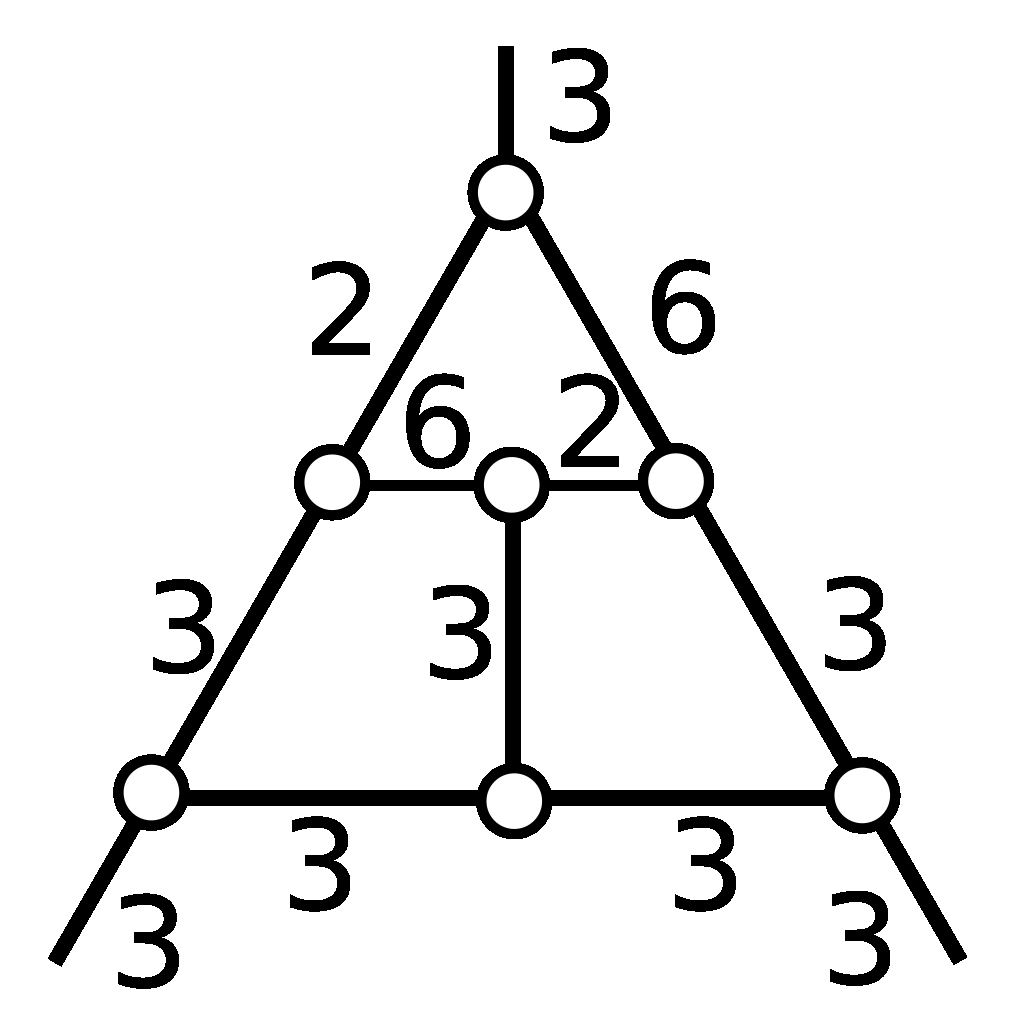
\includegraphics[width=0.8in, keepaspectratio]{./img/HexahedraWithSphericalFaces/cube/cube_b.jpg}
   \subcaption{}
   \label{}
  \end{minipage}
 \hspace*{\fill}
  \begin{minipage}[t]{0.15\textwidth}
   \centering
   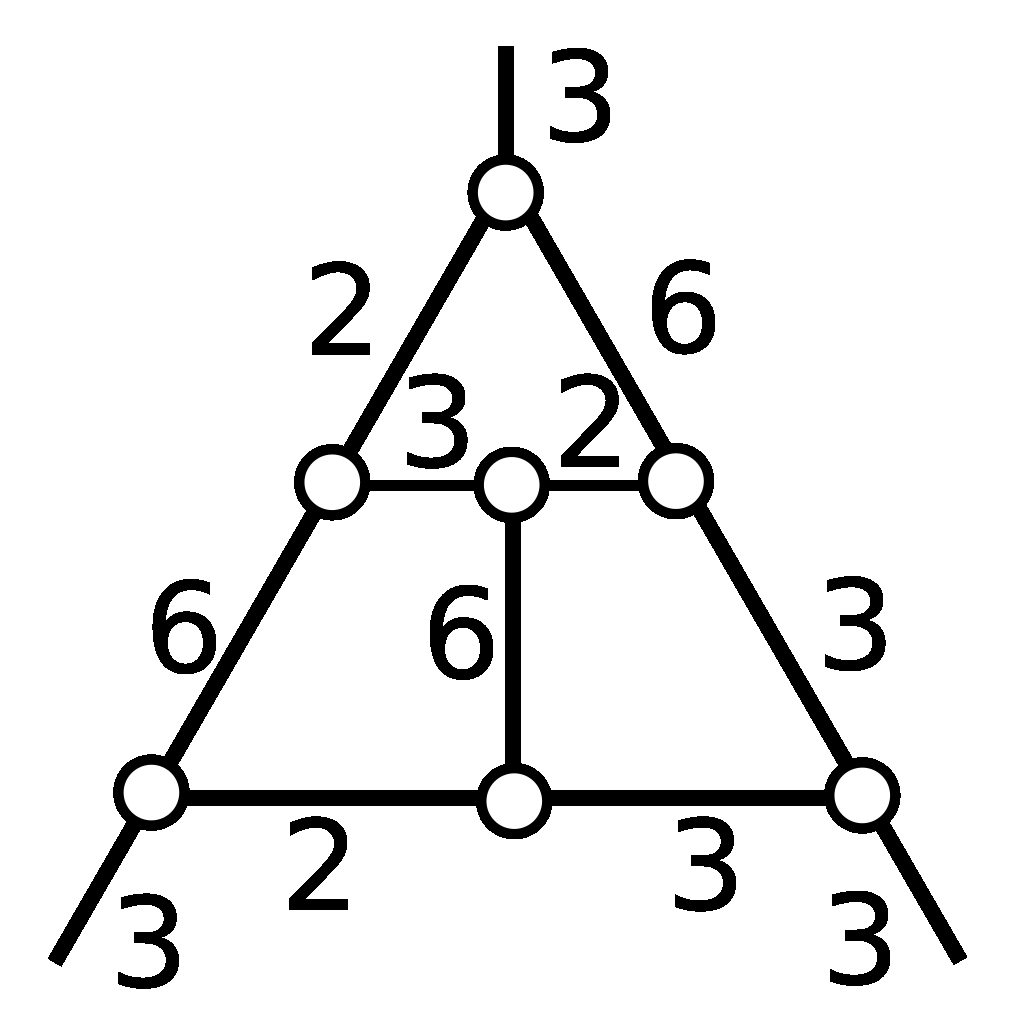
\includegraphics[width=0.8in, keepaspectratio]{./img/HexahedraWithSphericalFaces/cube/cube_c.jpg}
   \subcaption{}
   \label{fig:}
  \end{minipage}
 \hspace*{\fill}
  \begin{minipage}[t]{0.15\textwidth}
   \centering
   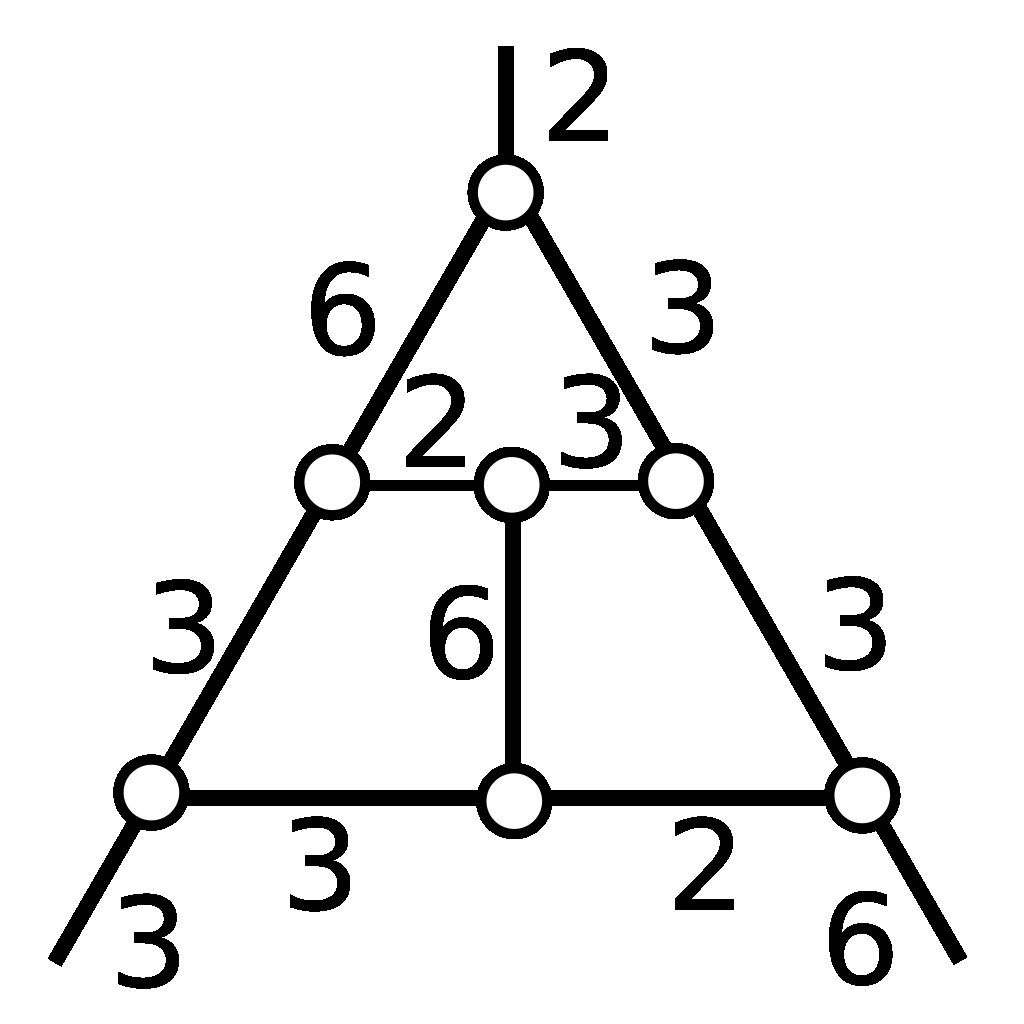
\includegraphics[width=0.8in, keepaspectratio]{./img/HexahedraWithSphericalFaces/cube/cube_d.jpg}
   \subcaption{}
   \label{fig:}
  \end{minipage}
 \hspace*{\fill}
  \begin{minipage}[t]{0.15\textwidth}
   \centering
   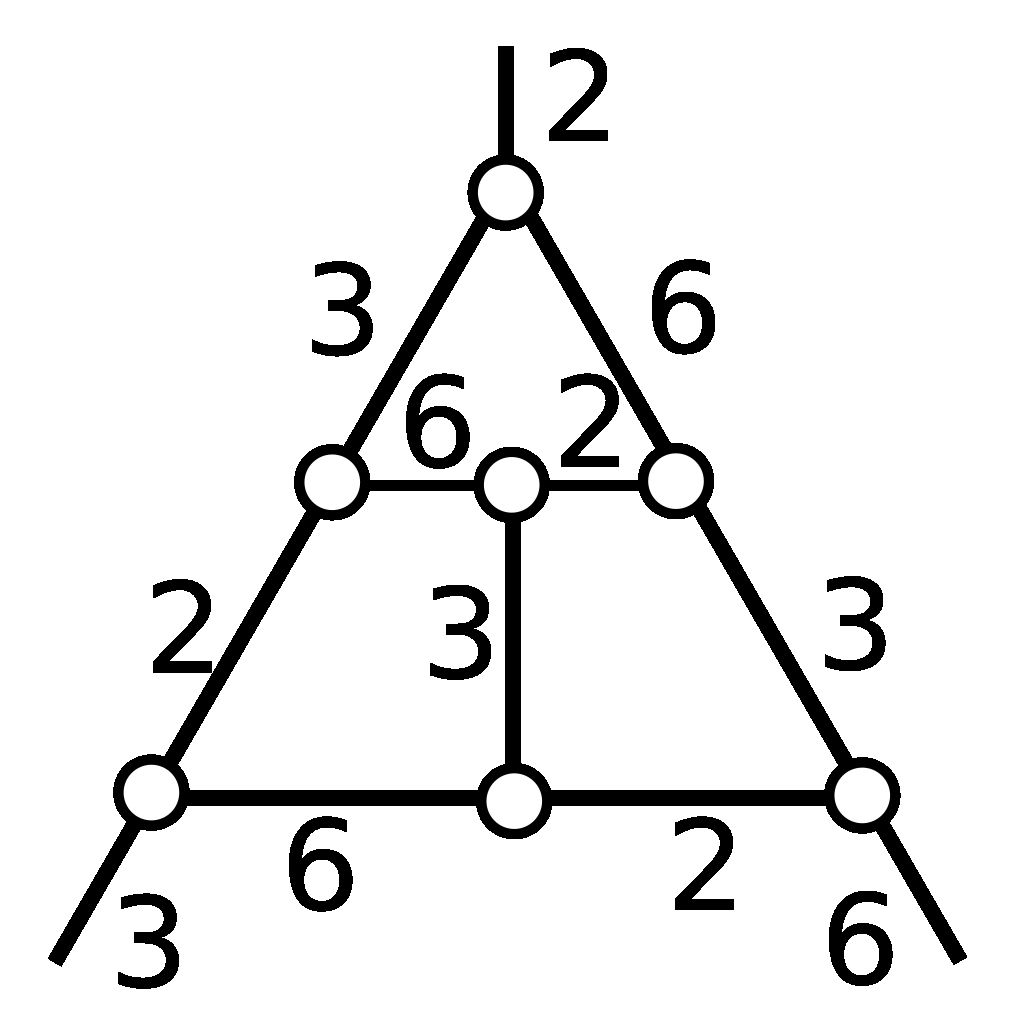
\includegraphics[width=0.8in, keepaspectratio]{./img/HexahedraWithSphericalFaces/cube/cube_e.jpg}
   \subcaption{}
   \label{fig:}
  \end{minipage}
 \hspace*{\fill}
\begin{minipage}[t]{0.15\textwidth}
   \centering
   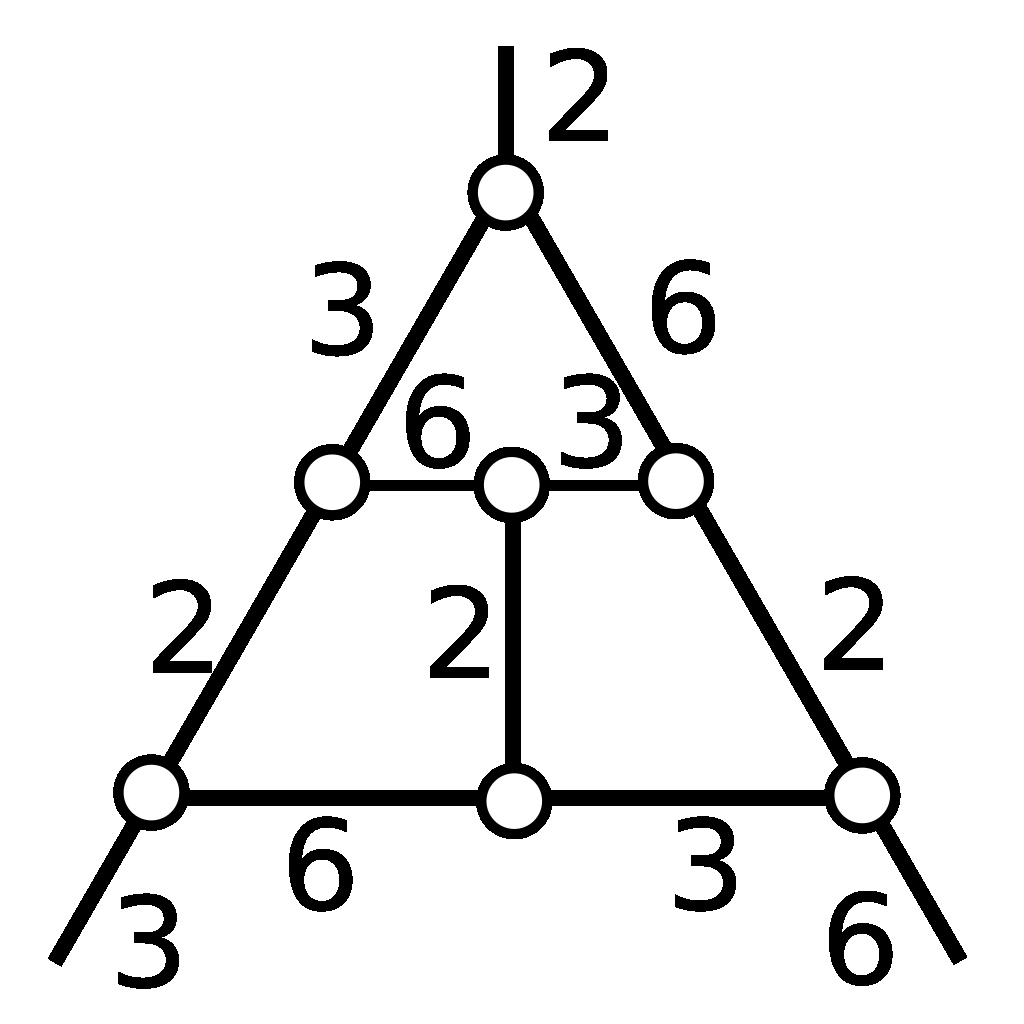
\includegraphics[width=0.8in,
 keepaspectratio]{./img/HexahedraWithSphericalFaces/cube/cube_f.jpg}
   \subcaption{}
   \label{fig:}
  \end{minipage}
 \hspace*{\fill}
  \begin{minipage}[t]{0.15\textwidth}
   \centering
   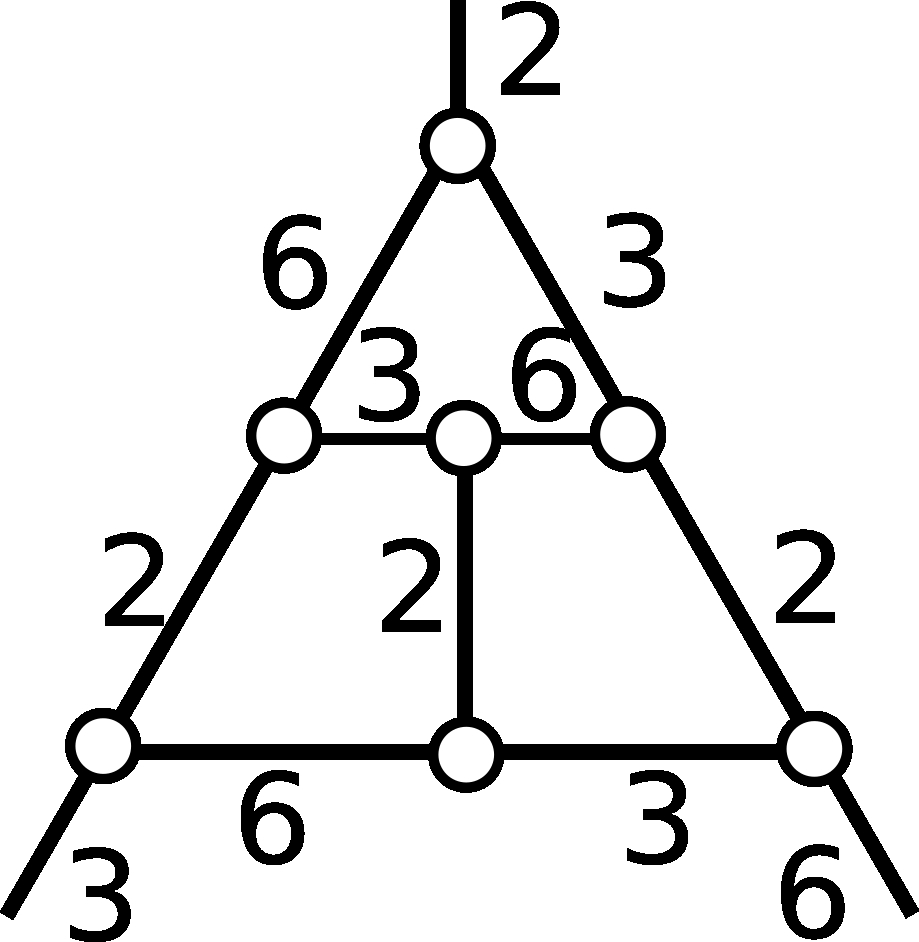
\includegraphics[width=0.8in,
   keepaspectratio]{./img/HexahedraWithSphericalFaces/cube/cube_g.jpg}
   \subcaption{}
   \label{fig:}
  \end{minipage}
  \hspace*{\fill}
  \begin{minipage}[t]{0.15\textwidth}
   \centering
   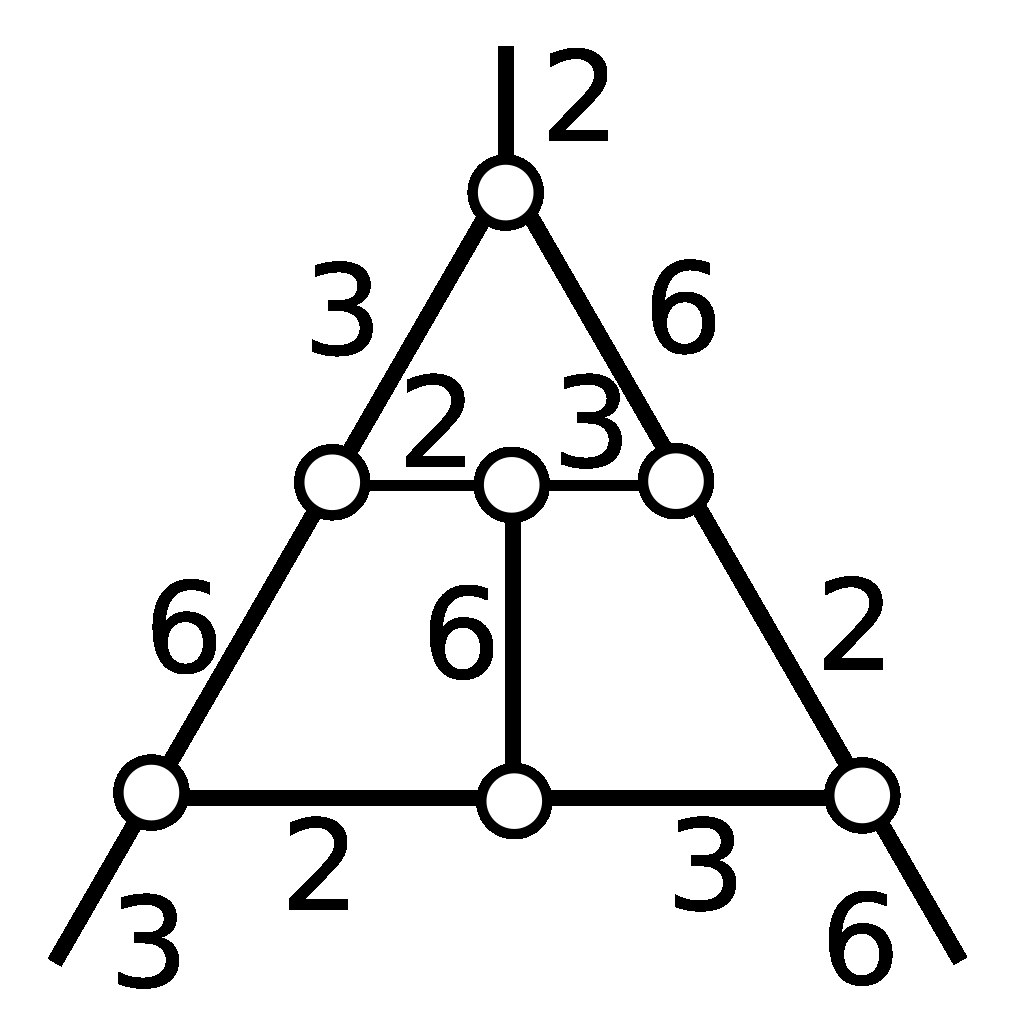
\includegraphics[width=0.8in, keepaspectratio]{./img/HexahedraWithSphericalFaces/cube/cube_h.jpg}
   \subcaption{}
   \label{}
  \end{minipage}
 \hspace*{\fill}
  \begin{minipage}[t]{0.15\textwidth}
   \centering
   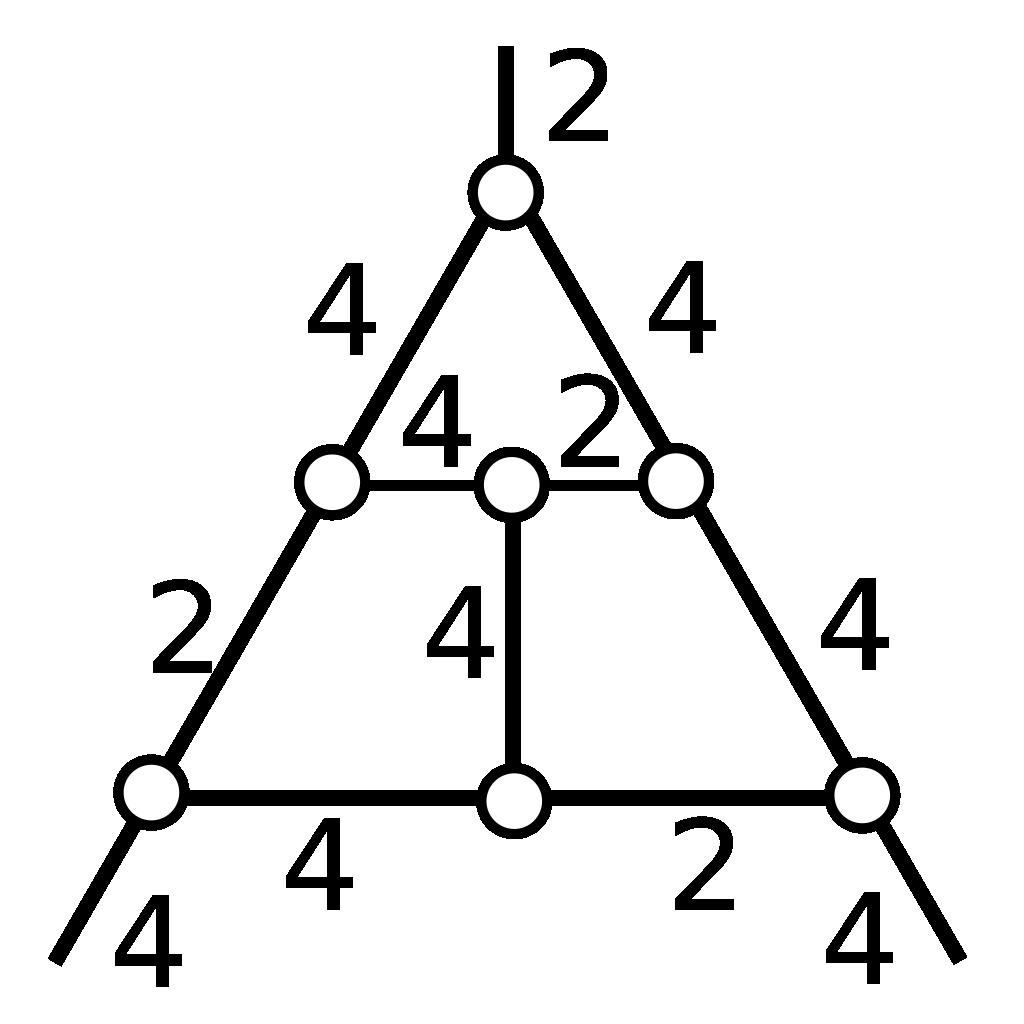
\includegraphics[width=0.8in, keepaspectratio]{./img/HexahedraWithSphericalFaces/cube/cube_i.jpg}
   \subcaption{}
   \label{fig:}
  \end{minipage}
 \hspace*{\fill}
  \begin{minipage}[t]{0.15\textwidth}
   \centering
   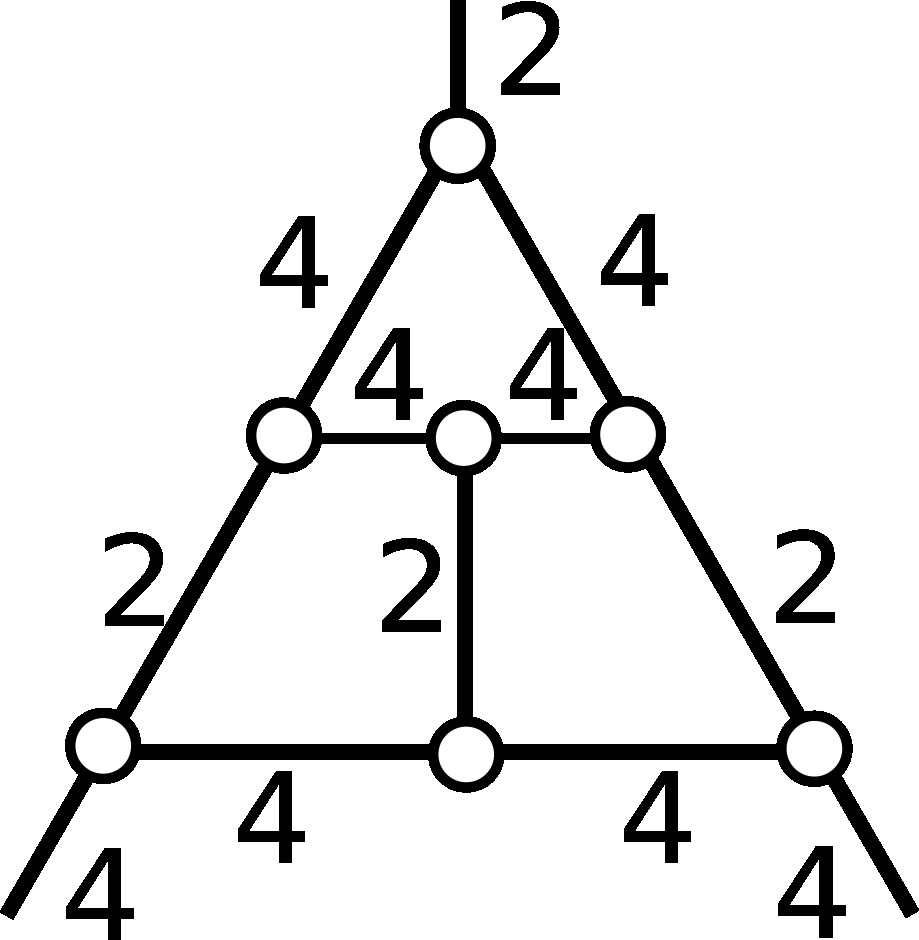
\includegraphics[width=0.8in, keepaspectratio]{./img/HexahedraWithSphericalFaces/cube/cube_j.jpg}
   \subcaption{}
   \label{fig:}
  \end{minipage}
 \hspace*{\fill}
  \begin{minipage}[t]{0.15\textwidth}
   \centering
   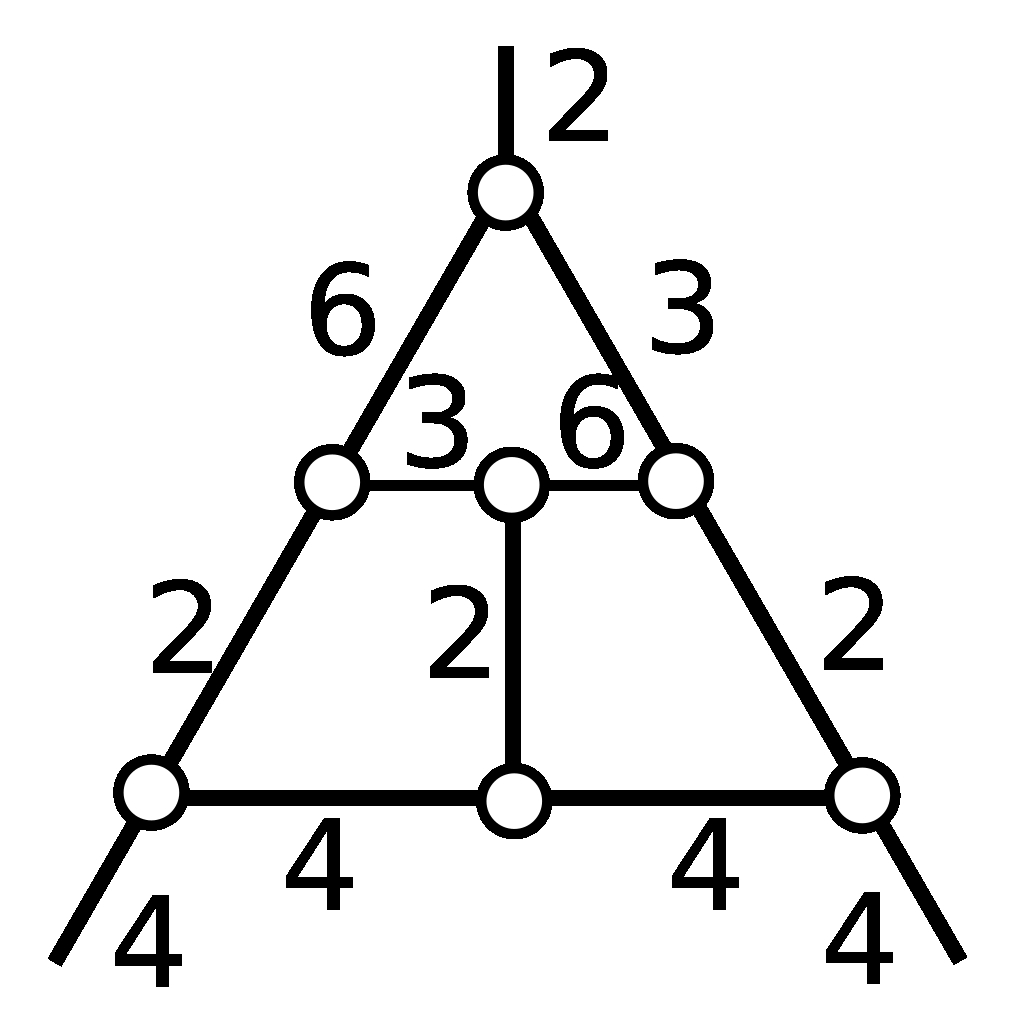
\includegraphics[width=0.8in, keepaspectratio]{./img/HexahedraWithSphericalFaces/cube/cube_k.jpg}
   \subcaption{}
   \label{fig:}
  \end{minipage}
 \hspace*{\fill}
  \caption{\textit{Cube-type}}
  \label{fig:cubeGraph}
 \end{minipage}
\end{figure}

We get this lemma only in a combinatorial way, so we omit the proof.

In order to represent a sphairahedron, we use a polyhedral graph, as
shown in Figure \ref{fig:cubeGraph}. The graph shows an infinite cube-type sphairahedron.
The black lines represent edges, and the circles represent
vertexes. The three radial edges connect the infinite vertex and finite
vertexes. Each of the numbers beside 
the edges means a natural number $n$ for the dihedral angle $\pi / n$

In this preview section, we introduce that there are seven types of
combinations of face angles. But here are 11. In fact, in case (f), (g),
(j), and (k), there is no polyhedron with these face-angles. See section \ref{paramSpace}.

\subsection{Constructing hexahedron}

We fix a set ($n_{ij}$) of face-angles and consider conformal equivalent
classes of polyhedra with (P1), (P2), (P3).

In the sequel, we suppose that $H = \infty$. (See Figure
\ref{fig:infTriangle}.) So the three
edges $HA, HB, HC$ are straight lines and are parallel to each other. We
assume that they are perpendicular to xy-plane.
Let ($x_A, y_B, z_z$), ..., ($x_G, y_G, z_G$) be coordinates of vertexes
A, B, ..., G (except $H$), respectively. Let $A'(x_A, y_A)$, ...,
$G'(x_G, y_G)$ be projection of these seven vertexes to the xy-plane.

We get immediately that $\angle C'A'B' = \theta_{13}, \angle A'B'C' =
\theta_{15}, \angle B'C'A'=\theta_{35}$. Remark that $\theta_{13} +
\theta_{15} + \theta_{35} = \pi$ by Lemma\ref{sum}.

Here we may assume that the radius of the circumcircle of $A'B'C'$ is 1,
that the circumcenter of $A'B'C'$ is $(0, 0, 0,)$ and that $A'$ is on
the x-axis. If it is not, by a proper M\"obius transformation(such that
it fixes the infinity point,) and it is easy to let the polyhedron
satisfy these conditions. By parallel transformation along the z-axis, we
may assume that $A$ is on xy-plane. (That is, $A = A'$ and $z_A = 0.$)

See Figure \ref{fig:infTriangle} again. $O_2, O_4, O_6$ are spheres. Let $O_i(x_i, y_i, z_i)$
and $r_i$ be the center and the radius of $O_i$ for $i = 2, 4, 6.$ About
the radius, we have the following proposition.

\begin{figure}[h!tbp]
 \begin{minipage}[t]{0.5\textwidth}
 \centering
 \includegraphics[width=3in, height=3in,
 keepaspectratio]{./img/HexahedraWithSphericalFaces/sideSlice.jpg}
 \caption{sideSlice}
 \label{fig:sideSlice}
 \end{minipage}
 \hspace*{\fill}
 \begin{minipage}[t]{0.5\textwidth}
  \centering
  \includegraphics[width=3in, height=3in,
  keepaspectratio]{./img/HexahedraWithSphericalFaces/abcTriangle.jpg}
  \caption{abcTriangle}
  \label{fig:abcTriangle}
 \end{minipage}
 \hspace*{\fill}
\end{figure}

\begin{proposition}\label{angles}
 \begin{align}
 r_2\sin\theta_{12} + r_4\sin\theta_{14} &= \overline{AB}^2 / (2\overline{A'B'})\notag\\
 r_4\sin\theta_{45} + r_6\sin\theta_{56} &= \overline{BC}^2 / (2\overline{B'C'})\tag{2.A}\label{2A}\\
 r_2\sin\theta_{23} + r_6\sin\theta_{36} &= \overline{CA}^2 / (2\overline{C'A'})\notag
 \end{align}
\end{proposition}

\begin{proof}
 In Figure \ref{fig:sideSlice}, the edge $AD = e_{12}$ is a circle with radius
 $r_2\sin\theta_{12}$, and the edge $DB e_{14}$ is a circle with radius
 ($r_4\sin\theta_{14}$.)
Two vertical lines $HA$ and $HB$ are tangent to these circles as in
 Figure \ref{fig:sideSlice},
 and we have 
 \begin{eqnarray*}
  \overline{AD} = 2 r_2 \sin\theta_{12} \cdot \overline{A'B'}/\overline{AB}\\
  \overline{DB} = 2 r_4 \sin\theta_{14} \cdot \overline{A'B'}/\overline{AB}
 \end{eqnarray*}
 Remark that $\cos(\angle BAB') =\overline{A'B'}/\overline{AB}.$ Clearly,
 $\overline{AD} + \overline{DB} = \overline{AB}$ holds, so it is easy to
 show the first formula of Proposition \ref{angles}. Others are shown in the same
 way.

\end{proof}

\begin{remark}
 If we regard (\ref{2A}) as a linear equation on $r_2, r_4, r_6$, the
 coordinate matrix of (\ref{2A}) is not singular. In fact,
 \begin{eqnarray*}
  \left| 
   \begin{array}{ccc}
    \sin\theta_{12} & \sin\theta_{14} & 0\\
    0               & \sin\theta_{45} & \sin\theta_{56}\\
    \sin\theta_{32} & 0               & \sin\theta_{36}
   \end{array}
  \right|
 \end{eqnarray*}
 is positive.
 If we fix three vertexes $A, B, C$, then always there are solutions of
 (\ref{2A}), but they may be non-positive. And, if $r_2$ or $r_4$ or $r_6$
 are too large, ($O_i$) doesn't form a hexahedron. For example, see
 subsection \ref{extend}. In this section, we know that $r_2, r_4, r_6$ are all
 'valid' if and only if parameters ($z_B, z_C$) are in the restricted area.

Next, we will obtain the coordinate of the centers of $O_2, O_4, O_6$.
Let $O_i'(x_i, y_i)$ be a projection of the center of the sphere $O_i$
 to xy-plane (for $i = 2, 4, 6$.)
\end{remark}

\begin{proposition}\label{angles}
 (1)$\angle O_2'A'B' = \pi/2 - \theta_{12}, \angle
 O'_2A'C'=\pi/2-\theta_{23}$.

  $\angle O_4'B'A' = \pi/2 - \theta_{14}, \angle O_4'B'C' = \pi/2 -
 \theta_{45}$.

 $\angle O_6'C'A' = \pi/2 - \theta_{36}, \angle O_6'C'A' = \pi/2 - \theta_{56}$.

 (2)$z_A = z_2 = 0$ and $\overline{A'O'_2} = \overline{AO_2} = r_2$

 $z_B = z_4$ and $\overline{B'O'_4} = \overline{BO_4} = r_4$

 $z_C = z_6$ and $\overline{C'O'_6} = \overline{CO_6} = r_6$
\end{proposition}

\begin{proof}
 (1) Since the face-angle of the plane $O_1$ and the sphere $O_2$ is
 $\theta_{12}$, the angle of a straight line $A'B'$ and a circle with
 center $O'_2$ and with radius $r_2$ is also $\theta_{12}$. It follows
 that $\angle O_2'A'B' = \pi/2 - \theta_{12}$(See Figure \ref{fig:abcTriangle}.)
 
 (2) The edge $AD = e_{12}$ is the intersection of a plane $O_1$ and a
 sphere $O_2$. This edge(= plane circle) is tangent to $AH$ (which is
 parallel to z-axis) at $A$, so a radius $AO_2$ of the sphere $O_2$ is
 perpendicular to $AH$. It follows that $z_A=z_2$ and that
 $\overline{A'O'_2} = \overline{AO_2}$ immediately.

 Using Lemma \ref{angles}(1), we can obtain all coordinates of $O_i$ from
 $\theta_{ij}$ and $r_i$ and $z_A, z_B, z_C$. In fact, the formula
 $\angle O'_2, A'B' = \pi/2 - \theta_{12}, \angle O'_{2}A'C' = \pi/2 -
 \theta_{23}$ means that the center $O_2'$ is a half-line with one
 end $A'$ as in Figure \ref{fig:abcTriangle}.
 And $\overline{A'O'_2} = \overline{AO_2} = r_2$ determines $A'$.
 So $O'_2$ is uniquely determined. From Lemma \ref{angles}(2), we get the
 z-coordinates $z_2$ of the center $O_2$ from $z_A(=0.)$ Hence a sphere
 $O_2$ is uniquely determined from $\theta_{ij}$'s and positive $r_2$
 and $z_A(= 0.)$
\end{proof}

\subsection{Compatibility}
In this way, for given parameters ($z_B,~z_C$) such that $r_2,~r_4,~r_6$
are all positive, we get the coordinates of three spheres 
$O_2, O_4, O_6$. But it is not trivial whether the 6-ple($O_1,~...,~O_6$) is
in $\tilde\varepsilon(n_{ij})$. (That is, we have to show that 
($O_1,..., O_6$) satisfies (P1), (P2), (P3).)

\begin{theorem}\label{compat}
 Fix $(n_{ij})_{(i, j)\in E}$(which is one of combination in Lemma
 \ref{combination})
 Fix three vertexes $A,~B,~C$. Assume that linear equations (\ref{2A}) have
 positive solutions. Then $O_1,~O_3,~O_5$ as in Figure \ref{fig:infTriangle} and
 $O_2,~O_4,~O_6$ as in Proposition \ref{angles} satisfy followings.
 \begin{description}
  \item[(1)] The face-angle of $O_2$ and $O_4$ (resp. $O_4$ and $O_6$,
             $O_2$ and $O_6$) is equal to $\theta_{24}$
             (resp. $\theta_{46}$, $\theta_{26}$.)
  \item[(2)] The intersecrion set of two spheres $O_2$, $O_4$ and a plane
             $O_1$ consists of only one point. The point is 
             $D = v_{124}$. Similarly other two vertexes $E = v_{245}$
             and $F = v_{236}$ are uniquely determined.
  \item[(3)] The intersection set of the three spheres $O_2, O_4, O_6$
             consists of only one point. The point is $G = v_{246}$.
             
  \item[(4)] $(O_1, ..., O_6) \in \tilde\varepsilon(n_{ij})$.
\end{description}
\end{theorem}

\begin{figure}[h!tbp]
 \begin{minipage}[t]{0.5\textwidth}
  \centering
  \includegraphics[width=3in, height=3in,
  keepaspectratio]{./img/HexahedraWithSphericalFaces/sideSliceDistance.jpg}
  \caption{}
  \label{fig:sideSliceDistance}
 \end{minipage}
 \hspace*{\fill}
 \begin{minipage}[t]{0.5\textwidth}
  \centering
  \includegraphics[width=3in, height=3in,
  keepaspectratio]{./img/HexahedraWithSphericalFaces/adb.jpg}
  \caption{}
  \label{fig:adb}
 \end{minipage}
 \hspace*{\fill}
\end{figure}

 
\begin{proof}
 (1) Let $\theta'_{24}$ be the face-angle of $O_2$ and $O_4$. From the
 law of cosine, we have
 \begin{align}
  \overline{O_2O_4}^2 = r_2^2 + r_4^2 - 2r_2r_4\cos(\pi-\theta'_{24}) \tag{2.B}\label{2B}
 \end{align}
From Figure \ref{fig:adb}, we get a formula
\begin{eqnarray*}
 \overline{O'_2O'_4}^2 = (\overline{A'B'} - r_2\sin\theta_{12}-
  r_4\sin\theta_{14})^2 + (-r_2\cos\theta_{12} + r_4 \cos \theta_{14})^2
\end{eqnarray*}
 Remark that $z_2 = z_A= 0, z_4 = z_B$. Then we have
\begin{eqnarray*}
 \overline{O_2O_4}^2 &=& \overline{O'_2O'_4}^2 + (z_2-z_4)^2\\
 &=&\overline{A'B'}^2 + 2 \overline{A'B'}(-r_2\sin\theta_{12} -
  r_4\sin\theta_{14}) + r^2_2 + r^2_4 -2r_2r_4\cos(\theta_{12} +
  \theta_{14}) + z^2_B
\end{eqnarray*}
Using (\ref{2B}) and $\overline{A'B'}^2 + (z_A-z_B)^2 = \overline{AB}^2$,
\begin{eqnarray*}
 \overline{AB}^2 + 2\overline{A'B'}(-r_2\sin\theta_{12} -
  r_4\sin\theta_{14}) - 2r_2r_4\{\cos(\theta_{12} + \theta_{14}) -
  \cos(\pi- \theta'_{24})\} = 0
\end{eqnarray*}
 $r_2, r_4$ satisfy (\ref{2A}) and they are positive, so we obtain
\begin{eqnarray*}
 \cos(\theta_{12} + \theta_{14}) = \cos(\pi - \theta'_{24})
\end{eqnarray*}
From Lemma \ref{sum}, $\theta_{12} + \theta_{14} + \theta_{24} = \pi$. It
 follows that $\theta_{24} = \theta'_{24}$. In the same way $\theta_{46}$
 (resp.$\theta_{26}$) is equal to the face-angle of $O_4$ and $O_6$(resp
 $O_2$ and $O_6$.)

(2) First we show that two edges $e_{12}$ and $e_{14}$ are mutually tangent
 on $O_1$. The radius of $e_{12}$(resp. $e_{14}$) is
 $r_2\sin\theta_{12}$ (resp. $r_4\sin\theta_{14}$). Let $d$ be the
 distance between two centers of two circles $e_{12}$, $e_{14}$. See
 Figure \ref{fig:sideSliceDistance}.

We have
 \begin{align*}
d^2&= (\overline{A'B'} - r_2\sin\theta_{12}-r_4\sin\theta_{14})^2 + \overline{BB'}^2\\
&= (\overline{A'B'} - \overline{AB}/(2\overline{A'B'}))^2 + \overline{BB'}^2\\
&= \overline{A'B'}^2 - \overline{AB}^2
  +\overline{AB}^4/(4\overline{A'B'}^2) + \overline{BB'}^2\\
&= \overline{AB}^4 / (4 \overline{A'B'}^2)\\
&=(r_2\sin\theta_{12} + r_4\sin\theta_{14})^2\\
d&= r_2\sin\theta_{12} + r_4\sin\theta_{14}
 \end{align*}
It means that $e_{12}$ and $e_{14}$ are mutually tangent.

Next we will show that the edge $e_{24}$ is tangent to both of $e_{12}$ and
 $e_{14}$. Assume that it is not. Then $e_{24}$ intersects to $O_1$
 twice.
(Remark that the tangent point of $e_{12}$ and $e_{14}$ is also on the
 circle $e_{24}$.) But all intersection points of $e_{24}$ and $O_1$ are
 on $e_{12}$ and $e_{14}$ by definition. This contradicts to the fact
 that $e_{12}$ is tangent to $e_{14}$. So the edge $e_{24}$ is tangent
 to both of $e_{12}$ and $e_{14}$. Similarly we will show it about $E$
 and $F$.

\begin{figure}[h!tbp]
  \begin{minipage}[t]{0.3\textwidth}
   \centering
   \includegraphics[width=2in, keepaspectratio]{./img/HexahedraWithSphericalFaces/threeCircles1.jpg}
   \subcaption{}
   \label{fig:}
  \end{minipage}
 \hspace*{\fill}
  \begin{minipage}[t]{0.3\textwidth}
   \centering
   \includegraphics[width=2in, keepaspectratio]{./img/HexahedraWithSphericalFaces/threeCircles2.jpg}
   \subcaption{}
   \label{fig:}
  \end{minipage}
  \hspace*{\fill}
  \begin{minipage}[t]{0.3\textwidth}
   \centering
   \includegraphics[width=2in, keepaspectratio]{./img/HexahedraWithSphericalFaces/threeCircles3.jpg}
   \subcaption{}
   \label{fig:}
  \end{minipage}
  \caption{\textit{}}
  \label{fig:threeCircles}
\end{figure}


(3) Let $\alpha$ be a plane containing three centers $O_2, O_4, O_6$. Let
 $C_2, C_4, C_6$ be three circles on $\alpha$ such that $C_i$ is the
 intersection of the sphere $O_i$ and the plane $\alpha$. ($i=2, 4, 6$.)
Let R be the radical point of $C_2, C_4, C_6$. There are three cases
 here.
(i) $R$ is inside if $C_2, C_4, C_6$.(ii) R is outside $C_2, C_4, C_6$.
(iii)$R$ is on $C_2, C_4, C_6$. (See Figure \ref{fig:threeCircles}.)

In the case (i), let three points $S_{24}, S_{46}, S_{26}$ be as in Figure
\ref{fig:threeCircles} (left). Here we have
$\angle O_2 S_{24} O_4 = \pi - \theta_{24}$,
because their face-angle of $O_2$ and $O_4$ is $\theta_{24}$.
In the same way, $\angle O_4 S_{46}O_6 = \pi - \theta_{46}$ and
$\angle O_2S_{26}O_6 = \pi-\theta_{26}$ hold. Hence

\begin{align*}
 \angle O_2 S_{24} O_4 + \angle O_4 S_{46} O_6 + \angle O_2 S_{26} O_6 = 3\pi -
 \theta_{24} - \theta_{46} - \theta_{26} = 2\pi.
\end{align*}

On the other hand, from Figure \ref{fig:threeCircles} (left)

\begin{align*}
 \angle O_2 S_{24} O_4 &< \angle O_2 R O_4\\
 \angle O_2 S_{24} O_4 &< \angle O_2 R O_4\\
 \angle O_2 S_{24} O_4 &< \angle O_2 R O_4\\
\end{align*}
and
\begin{align*}
 \angle O_2 R O_4 + \angle O_4 R O_6 + \angle O_2 R O_6 = 2\pi
\end{align*}
This is a contradiction. So this case cannot happen. In the same way,
 the case (ii) cannot happen. These follow that the radical point $R$
 is on the intersection of three circles $C_2, C_4, C_6.$ This means that
 $R$ is the unique intersection of 3 spheres $O_2, O_4, O_6$. This must
 be $G$.

(4) The 6-pre ($O_1, ..., O_6$) satisfies (P1) by definition.

(P2): For $(i, j) = (1, 3), (3, 5), (1, 5)$, it is good because we first
 take a triangle prism (consisting of $O_1, O_3, O_5$) with face-angles
 $\theta_{13}, \theta_{35}, \theta_{15}.$ 
For $(i, j) = (1, 2), (1, 4), (4, 5), (5, 6), (2, 3), (3, 6)$, it is
 good from Lemma\ref{angles}. In other cases, it is good from Theorem
 \ref{compat}(1).

(P3): At $H = \infty, AH, BH, CH$ are parallel lines, so they are tangent
 at $\infty$. At $A, B, C,$ Proposition \ref{angles} (2) follows that three edges
 with each vertex are tangent to each other. At $D, E, F, G,$ we have
 shown it in Theorem \ref{compat}(2)(3). 
\end{proof}

\subsection{Parameter space}\label{paramSpace}
In this subsection, we first consider in the case that $n_{ij} = 3$ for all
$(i, j) \in E$. (That is, in case (a) in Lemma \ref{combination}.) There
are 11 cases in Lemma \ref{combination}.
The case (a) is not a special case, and we can make
similar observation in other cases.
The linear equations (\ref{2A}) are:
\begin{align*}
 r_2 + r_4 &= (3 + z_B^2) / 3 \\
 r_4 + r_6 &= (3 + (z_B - z_C)^2 ) / 3 \\
 r_2 + r_6 &= (3 + z_C^2) / 3
\end{align*}

Here $\overline{A'B'} = \overline{B'C'} = \overline{A'C'} = \sqrt{3}$
because $\Delta{A'B'C'}$ is a regular triangle and the radius of the
circumcircle is 1.(In all cases, $\overline{A'B'} = 2\sin\theta_{35},
\overline{B'C'} = 2\sin\theta_{13}, \overline{A'C'} = 2\sin\theta_{15}$.)
We solve these equations, and we have 
\begin{align*}
\begin{cases}
 r2 &= (-2z_Bz_C + 2Z^2_C + 3) / 6 \\
 r4 &= (2z_Bz_C + 3) / 6 \tag{2.C}\label{2C}\\
 r6 &= (2z^2_B - 2z_Bz_c + 3) / 6.
 \end{cases}
\end{align*}
First we assume that $r_2, r_4, r_6$ are positive. This condition is
equivalent to the followings.
\begin{align*}
\begin{cases}
 -3 / 2 &< -z_Bz_C + z^2_C\\
 -3 / 2 &< z_Bz_C \tag{2.D}\label{2D}\\
 -3 / 2 &< z^2_B - z_Bz_C
\end{cases}
\end{align*}
So we assume (3.B). We will determine $O_1, ... , O_6$ as in the
previous section. It is clear that six faces $O_1, ... , O_6$ surround
a hexahedron if and only if $O_2$ doesn't interest to $O_5$ nor $O_3$
doesn't intersect to $O_4$ nor $O_1$ doesn't intersect to $O_6$.

$O_2$ doesn't interest to $O_5$ if and only if the distance from the center
of the sphere $O_2$ to the plane $O_5$ is more than $r_2$. In this case,
the distance is $3 / 2 - r_2$ and hence $O_2$ doesn't intersect to $O_5$
if and only if $r_2 < 3/4$. In the same way $r_4 < 3/4$ and $r_6 <
3/4$. These three inequalities are equivalent to
\begin{align*}
\begin{cases}
 -z_Bz_C + z^2_C < 3 / 4\\
 z_Bz_C < 3 / 4 \tag{2.E}\label{2E}\\
 z^2_B - z_B z_C < 3/ 4
\end{cases}
\end{align*}

\begin{figure}[h!tbp]
 \begin{minipage}[t]{0.5\textwidth}
 \centering
 \includegraphics[width=2in,
 keepaspectratio]{./img/graph/cubeA.jpg}
 \caption{}
 \label{fig:graphCubeA}
 \end{minipage}
 \hspace*{\fill}
 \begin{minipage}[t]{0.5\textwidth}
  \centering
  \includegraphics[width=2in,
  keepaspectratio]{./img/graph/cubeALimit.jpg}
  \caption{}
  \label{fig:graphCubeALimit}
 \end{minipage}
 \hspace*{\fill}
\end{figure}

\begin{align*}
(1)& z_Bz_C = 3/4\\
(2)& z_C^2 - z_B z_C = 3/4\\
(3)& z_B^2 - z_B z_C = 3/4
\end{align*}

See Figure \ref{fig:graphCubeA} ($z_B, z_C$) in the shaded area of this figure satisfies
all of(\ref{2D}) and (\ref{2E}) and $z_B \geq 0$.

In case (a), the original three parameters $z_A, z_B, z_C$ have symmetry,
because $O_1, O_3, O_5$ form a \textit{regular} triangle prism.
If $z_C < 0$, then we exchange the roles of $z_A$ and $z_C$ and we can reduce
($z_B, z_C$) to ($z_B - z_C, -z_C$) in the case of $z_C > 0$.
If $0 \leq z_C < z_B$, then we exchange the roles of $z_B$ and $z_C$, 
and we can reduce $(z_B, z_C)$ to $(z_C, z_B)$ in case of 
$z_B < z_C$. If $z_B \leq z_C < 2z_B$ then we exchange the roles of
$z_A$ and $z_C$ and we can reduce($z_B, z_C$) to ($z_C-z_B,z_C$) in case
of $z_C \geq 2z_B$. In this way, the correct parameter space is as in
Figure \ref{fig:graphCubeALimit}.

Here two hyperbola $z^2_C - z_Bz_C = 3/4$ and $z_B z_C = 3/4$ intersects
at ($\sqrt{6} / 4, \sqrt{6}/2$) and this point is on the straight line
$z_C=2z_B$. In Figure \ref{fig:graphCubeALimit}, points on $z^2_C - z_Bz_C = 3/4$ aren't
contained in the area. When ($z_B, z_C$) is on this parabola, the face
$O_2$ is tangent to $O_5$. Moreover when
$(z_B, z_C) = (\sqrt{6} / 4, \sqrt{6}/2)$, the face $O_3$ is also tangent
to $O_4$.

\begin{figure}[h!tbp]
 \begin{minipage}[]{0.5\textwidth}
 \centering
 \includegraphics[width=2in,
 keepaspectratio]{./img/graph/cubeB.jpg}
 \caption{}
 \label{fig:graphCubeB}
 \end{minipage}
 \hspace*{\fill}
 \begin{minipage}[]{0.5\textwidth}
  case(b)
  \centering
  \begin{align*}
   (1)& -2\sqrt{3} z_B z_C + 54 - 30\sqrt{3} = 0\\
   (2)& -3z_B^2 + 4 z_B z_C + 15/4 = 0\\
   (3)& +2z_B z_C - 3z_C^2 + 3/4 = 0
  \end{align*}
 \end{minipage}
\end{figure}

\begin{figure}[h!tbp]
 \begin{minipage}[]{0.5\textwidth}
 \centering
 \includegraphics[width=2in,
 keepaspectratio]{./img/graph/cubeC.jpg}
 \caption{}
 \label{fig:graphCubeC}
 \end{minipage}
 \hspace*{\fill}
 \begin{minipage}[]{0.5\textwidth}
  \centering
  case(c)
  \begin{align*}
   (1)& -\sqrt{3}z_B^2 - 2\sqrt{3}z_Bz_C + 90 - 51\sqrt{3} = 0\\
   (2)& -3\sqrt{3}z_B^2 + 4\sqrt{3}z_B z_C + 90 - 48\sqrt{3} = 0\\
   (3)& z_B^2 + 2 z_B z_C - 5z_C^2 + 9/4 = 0
  \end{align*}
 \end{minipage}
 \hspace*{\fill}
\end{figure}

\begin{figure}[h!tbp]
 \begin{minipage}[]{0.5\textwidth}
 \centering
 \includegraphics[width=2in,
 keepaspectratio]{./img/graph/cubeD.jpg}
 \caption{}
 \label{fig:graphCubeD}
 \end{minipage}
 \hspace*{\fill}
 \begin{minipage}[]{0.5\textwidth}
  \centering
  case(d)
  \begin{align*}
   (1)& -3z_B^2 - 6z_B z_C - z_C^2 -60 +36\sqrt{3} = 0\\
   (2)& -15 z_B^2 + 6z_Bz_C + z_C^2 - 120 + 72\sqrt{3} = 0\\
   (3)& 3z_B^2 + 6z_Bz_C - 5z_C^2 - 120 + 72 \sqrt{3} = 0
  \end{align*}
 \end{minipage}
 \hspace*{\fill}
\end{figure}

\begin{figure}[h!tbp]
 \begin{minipage}[]{0.5\textwidth}
 \centering
 \includegraphics[width=2in,
 keepaspectratio]{./img/graph/cubeE.jpg}
 \caption{}
 \label{fig:graphCubeE}
 \end{minipage}
 \hspace*{\fill}
 \begin{minipage}[]{0.5\textwidth}
  \centering
  case(e)
  \begin{align*}
   (1)& -6z_Bz_C - z_C^2 + 9/4 = 0\\
   (2)& 7z_B^2 - 6z_Bz_C - z_C^2 - 3 = 0\\
   (3)& z_Bz_C - z_C^2 - 24 + 14\sqrt{3} = 0
  \end{align*}
 \end{minipage}
 \hspace*{\fill}
\end{figure}

\begin{figure}[h!tbp]
 \begin{minipage}[]{0.5\textwidth}
 \centering
 \includegraphics[width=2in,
 keepaspectratio]{./img/graph/cubeH.jpg}
 \caption{}
 \label{fig:graphCubeH}
 \end{minipage}
 \hspace*{\fill}
 \begin{minipage}[]{0.5\textwidth}
  \centering
  case(h)
  \begin{align*}
   (1)& -3z_B^2 - 2z_Bz_C + 3/4 = 0\\
   (2)& -3z_B^2 + 3 z_Bz_C + 2 = 0\\
   (3)&  3z_B^2 + 2z_Bz_C -5z_C^2 + 3 = 0
  \end{align*}
 \end{minipage}
 \hspace*{\fill}
\end{figure}

\begin{figure}[h!tbp]
 \begin{minipage}[]{0.5\textwidth}
 \centering
 \includegraphics[width=2in,
 keepaspectratio]{./img/graph/cubeI.jpg}
 \caption{}
 \label{fig:graphCubeI}
 \end{minipage}
 \hspace*{\fill}
 \begin{minipage}[]{0.5\textwidth}
  \centering
  case(i)
  \begin{align*}
   (1)& -2z_Bz_C - z_C^2 + 1 = 0\\
   (2)& -3z_B^2 + 2 z_B z_C + z_C^2 + 2 = 0\\
   (3)& z_Bz_C - z_C^2 - 8 + 6\sqrt{2} = 0
  \end{align*}
 \end{minipage}
 \hspace*{\fill}
\end{figure}

In the same way, we have a similar result in case 
$(b), (c), (d), (e), (h), (i)$. 
The figures above are parameter space in each case.
We show parameter spaces not considering symmetry.

In case $(f), (g), (j), and (k)$, there is no solution of $(z_B, z_C)$
to be a hexahedron. In fact, in case (f),
\begin{align*}
\begin{cases}
 0 &< \dfrac{z_Bz_C}{\sqrt{3}} < \dfrac{\sqrt{3}}{4} \\
 0 &< \dfrac{1 + z^2_B - z_Bz_C}{2} < \dfrac{1}{2} \\
 0 &< \dfrac{3 + z^2_C - z_Bz_C}{2\sqrt{3}} < \dfrac{\sqrt{3}}{2}.
\end{cases}
\end{align*}

In case (g),

\begin{align*}
\begin{cases}
0 &< \dfrac{z_Bz_C}{2} < \dfrac{\sqrt{3}}{2 + \sqrt{3}} \\
0 &< \dfrac{2 + 2z^2_B - z_Bz_C}{4} < \dfrac{1}{2} \\
0 &< \dfrac{\sqrt{3}(6 + 2z^2_C - 3z_Bz_C)}{12} < \dfrac{\sqrt{3}}{2}
\end{cases}
\end{align*}

In case (j),

\begin{align*}
 \begin{cases}
  0 &< \dfrac{z_Bz_C}{2} < \dfrac{1}{2}\\
  0 &< \dfrac{\sqrt{2}(2 + z^2_B - z_B z_C)}{4} < \dfrac{\sqrt{2}}{2}\\
  0 &< \dfrac{\sqrt{2}(2 + z^2_C - z_B z_C)}{4} < \dfrac{\sqrt{2}}{2}
 \end{cases}
\end{align*}

In case (k),

\begin{align*}
 \begin{cases}
  0 &< \dfrac{2z_Bz_C}{\sqrt{6} + \sqrt{2}} < \dfrac{1}{\cos(\pi/12+1)}\\
  0 &< \dfrac{\sqrt{2}(2 (1 + \sqrt{3}) + (1 + \sqrt{3})z^2_B -2z_Bz_C)}
  {2(\sqrt{6} + \sqrt{2})} < \dfrac{\sqrt{2}}{2}\\
  0 &< \dfrac{\sqrt{2}(2 (1 + \sqrt{3}) + (1 + \sqrt{3})z^2_C
  -2\sqrt{3}z_Bz_C)}
  {2(\sqrt{6} + \sqrt{2})} < \dfrac{\sqrt{2}}{2}
 \end{cases}
\end{align*}
In these cases, there is no answer for ($z_B, z_C$).

We complete the proof of the main Theorem \ref{main}.

\subsection{Group $G$ and the limit set $\Delta(G)$}
Let $\gamma_i \in \text{M\"ob}(S^3)$ be the inversion of $O_i$ for $i =
1,...,6$.
Let $G'$ be a group generated by $\gamma_i$'s. From Condition (P2), we
have relations
\begin{align*}
 (\gamma_i \gamma_j)^{n_{ij}} = 1
\end{align*}
for $(i, j) \in E.$ (Here $1$ is the identity map.) If $(i, j) \notin E$,
there is no relation between $\gamma_i$ and $\gamma_j$.
And at each vertex, three edges with the vertex are mutually tangent.
There are no more relations. So we have that
\begin{align*}
 \tilde G = <\gamma_1, ...,\gamma_6~|~(\gamma_i\gamma_j)^{n_{ij}} = 1 \text{for}
 (i, j) \in E.>
\end{align*}
The length of all relations is even, so that we can consider a set $G = G(P)$
of elements of even length. $G$ is a subset of $G'$. Here we remark
that each $\gamma_i$ is an inversion, and it is orientation reversing. So
each element of $G$ is orientation preserving M\"obius transformation.
It follows that $G$ is a subset of M\"ob$_+(S^3)$.

In the previous subsection, we got a parameter space for $P$ to be a
hexahedron with the initial conditions. Here are some pictures of the
limit sets $\Lambda(G)$. However, if we take $O_1, ..., O_6$ as in the
previous section, the limit set contains an infinity point $\infty$. So
we transform $O_1, ..., O_6$ by an inversion of a proper sphere in
order to make $\Lambda(G)$ doesn't contain the infinity point.

Only when $(z_B, z_C) =(0, 0), \Lambda(G)$ is a round sphere, and hence
$G$ is fuchsian. In other cases, we get a homotopy to the case 
$(z_B, z_C) = (0, 0)$, we know that $G$ is quasi-fuchsian.

\subsection{Extended Schottky group for a cube with spherical faces}\label{extend}
If $(O_1, ..., O_6)$ gives a polyhedron with conditions
$(P1), (P2), (P3)$.
These spheres also define a Schottky type subgroup of M\"ob$_+(S^3)$ 
only in case (a). Indeed we have the following  proposition.

\begin{proposition}
Let $\{n_{ij}\}$ be of type (a) in Lemma \ref{combination}. Then there exist three
 (orientation preserving) transformations $f_1, f_2, f_3$ such that
 \begin{description}
  \item[(1)] $f_1$ maps the inside of $O_1$ onto the outside of
             $O_6$, $f_1(H) = C$, $f_1(A) = F$,  $f_1(D) = G$, and
             $f_1(B) = E$.
  \item[(2)] $f_2$ maps the inside of $O_3$ onto the outside of
             $O_4$, $f_2(H) = B$, $f_2(A) = D$,  $f_2(F) = G$, and
             $f_2(C) = E$.             
  \item[(3)] $f_3$ maps the inside of $O_5$ onto the outside of
             $O_2$, $f_3(H) = A$, $f_3(B) = D$,  $f_3(E) = G$, and
             $f_3(C) = F$.
\end{description}
\end{proposition}

Let $H$ be a sub group of M\"ob$_+(S^3)$ generated by $f_1, f_2,
f_3$. This proposition follows that
\begin{align*}
 H = <f_1, f_2, f_3~|~(f_1f_2)^3 = (f_2f_3)^3 = (f_1f_3)^3 = e>.
\end{align*}
It is easy to show that the fundamental domain of $H$ is a polyhedron
surrounded by the initial spheres. The limit set $H$ is the same as that
of $G$.

\begin{proof}
See Figure \ref{fig:infTriangle}. Since we assume that $n_{ij} = \pi/3$, we have
\begin{align*}
 A(1, 0, 0), B(-\frac{1}{2}, \dfrac{\sqrt{3}}{2}, z_B), C(-\frac{1}{2}, -\frac{\sqrt{3}}{2}, z_C).
\end{align*}
\end{proof}

Let $O_2$ be the center of the spheres $O_2$, then we have
\begin{align*}
 O_2(1 - r_2, 0, 0).
\end{align*}
From Lemma\ref{eightVertexes}, 7 points A, B, C, D, E, F, G lie on one plane. D is on
the segment $AB$ and
\begin{align*}
 AD : DB = r_2\sin\theta_{12} : r_4\sin\theta_{14} = r_2 : r_4
\end{align*}
See Figure \ref{fig:sideSlice}. In the same way, we have
\begin{align*}
 BE : EC &= r_4\sin\theta_{45} : r_6\sin\theta_{56} = r_4:r_6\\
 CF : FA &= r_6\sin\theta_{36} : r_2\sin\theta_{23} = r_6:r_2
\end{align*}
Using these, we have coordinates of $E$. In fact,
\begin{align*}
 E(-\dfrac{1}{2},\dfrac{\sqrt{3}}{2}\dfrac{r_6-r_4}{r_6 + r_4},
 \dfrac{z_Br_6 + z_C r_4}{r_6 + r_4}).
\end{align*}
And we have
\begin{align*}
 \dfrac{AD}{DB} \cdot \dfrac{BE}{EC} \cdot \dfrac{CF}{FA} = \dfrac{r_2r_4r_6}{r_4r_6r_2} = 1.
\end{align*}
From Ceva's theorem, the three lines $AE$, $BF$, and $CD$ meet at one
point. Let $G'$ be the intersection. Using Menelaus's theorem, we have
$AG':G'E = r_2r_4 + r_2r_6:r_4r_6$ and
\begin{align*}
 G' = \dfrac{1}{R}(r_4r_6 - \dfrac{1}{2}(r_2r_4 + r_2r_6), 
 \dfrac{\sqrt{3}}{2}r_2(r_6 - r_4), r_2(z_Br_6 + z_Cr_4)),
\end{align*}
where $R = r_2r_4 + r_4r_6 + r_6r_2.$ It follows that
\begin{align*}
 \overline{O_2G'}^2 = (1 - r_2 - \dfrac{1}{2R}(2r_4r_6 - (r_2r_4 +
 r_2r_6)))^2 + \dfrac{3r^2_2}{4R^2}(r_6 - r_4)^2 +
 \dfrac{r_2^2}{R^2}(z_Br_6 + z_Cr_4)^2
\end{align*}
Using Proposition \ref{angles}, we have $\overline{O_2G'} = r_2$.
Remark that we
use equations $z_B^2 = 3(r_2 + r_4 - 1), z_C^2 = 3(r_2 + r_6 - 1)$, and
$2z_Bz_C = 6r_2 - 3$.

In the similar way, we get $\overline{O_4G'} = r_4$ and 
$\overline{O_6G'} = r_6$. These mean that $G' = G$.

From Lemma \ref{sameCircle}, $B, D, G, E$ are on one circle. Hence
$CE \cdot CB = CG \cdot CD$. In the same way, we obtain 
$CG \cdot CD = CF \cdot CA$. So let $O$ be a sphere with center $C$ and
radius $\sqrt{CE \cdot CB}$ and let $f_O$ be the inversion of $O$.
The above two equations follows that
\begin{align*}
 f_O: A \mapsto F, D \mapsto G, B \mapsto E, H \mapsto C.
\end{align*}
Let $f_{O_1}$ be the inversion of $O_1$. $f_{O_1}$ fixes $H, A, D, B$.
Let $f_1 := f_O \circ f_{O_1}$.
$f_1$ is an orientation preserving M\"obius transformation and
\begin{align*}
 f_1 : A \mapsto F, D \mapsto G, B \mapsto E, H \mapsto C.
\end{align*}
It is easy to check that $f_1(O_1) = O_6$ because a sphere is determined
by four points on it. And also, $f_1$ maps the inside of $O_1$ to the
outside of $O_6$. Here the inside of $O_1$ means the area which doesn't
contain the consistent prism of $O_1, O_3, O_5$. We finish the
proof.

Remark:
In other cases $(b),...,(j)$, we don't have a similar result. Three
segments $AE, BF, CD,$ meet at one point only in case $(a), (f), (j)$, but
there isn't a parameter space in cases $(f)$ nor $(j)$.
% ここまで


\section{Various Sphairahedra}

In this section, we show other types of sphairahedra based on the
number of faces up to six.
We can obtain other sphairahedra in a similar manner to cube-type
sphairahedron.


\subsection{Pentahedron}

The pentahedron has two types. They are a pentahedral pyramid and pentahedral prism.

\subsubsection{pyramid}

\begin{figure}[h!tbp]
  \begin{minipage}[t]{0.5\textwidth}
   \centering
   \includegraphics[width=1in, keepaspectratio]{./img/HexahedraWithSphericalFaces/pentahedralPyramid/pyramid.jpg}
   \caption{pentahedral pyramid}
   \label{}
  \end{minipage}
 \hspace*{\fill}
  \begin{minipage}[t]{0.5\textwidth}
   \centering
   \includegraphics[width=1in, keepaspectratio]{./img/HexahedraWithSphericalFaces/pentahedralPyramid/faces.jpg}
   \caption{Graph}
   \label{fig:tetrahedronFaces}
  \end{minipage}
 \hspace*{\fill}
\end{figure}


\begin{figure}[h!tbp]
 \begin{minipage}[t]{0.24\textwidth}
   \centering
   \includegraphics[width=1in,
   keepaspectratio]{./img/HexahedraWithSphericalFaces/pentahedralPyramid/a.jpg}
   \subcaption{}
   \label{fig:}
 \end{minipage}
 \hspace*{\fill}
 \begin{minipage}[t]{0.24\textwidth}
   \centering
   \includegraphics[width=1in, keepaspectratio]{./img/HexahedraWithSphericalFaces/pentahedralPyramid/b.jpg}
   \subcaption{}
   \label{}
 \end{minipage}
 \hspace*{\fill}
 \caption{\textit{Graph of the Pentahedral pyramid.}}
  \label{fig:}
\end{figure}

\begin{figure}[H]
 \begin{minipage}{0.5\textwidth}
  \begin{minipage}[t]{0.24\textwidth}
   \centering
   \includegraphics[width=1.35in, height=1.35in, keepaspectratio]{./img/sphairahedron/pentahedralPyramid/sphairahedronFinite.jpg}
   \subcaption{\textit{Sphairahedron}}
  \end{minipage}
  \hspace*{\fill}
  \begin{minipage}[t]{0.24\textwidth}
   \centering
   \includegraphics[width=1.35in, height=1.35in, keepaspectratio]{./img/sphairahedron/pentahedralPyramid/limitsetFinite.jpg}
   \subcaption{\textit{Limit set}}
  \end{minipage}
  \hspace*{\fill}
  \caption{\textit{Finite tetrahedron type(a).}}
  \label{fig:pentahedralPyramidFinite}
 \end{minipage}
 \hspace*{\fill}
 \begin{minipage}{0.5\textwidth}
  \begin{minipage}[t]{0.24\textwidth}
   \centering
   \includegraphics[width=1.35in, height=1.35in, keepaspectratio]{./img/sphairahedron/pentahedralPyramid/sphairahedronInf.jpg}
   \subcaption{\textit{Sphairahedron}}
  \end{minipage}
  \hspace*{\fill}
  \begin{minipage}[t]{0.24\textwidth}
   \centering
   \includegraphics[width=1.35in, height=1.35in, keepaspectratio]{./img/sphairahedron/pentahedralPyramid/limitsetInf.jpg}
   \subcaption{\textit{Limit set}}
  \end{minipage}
  \hspace*{\fill}
  \caption{\textit{Infinite pentahedral pyramid type(a).}}
  \label{fig:pentahedralPyramidInf}
 \end{minipage}
\end{figure}

\begin{figure}[H]
 \begin{minipage}{0.5\textwidth}
  \begin{minipage}[t]{0.24\textwidth}
   \centering
   \includegraphics[width=1.35in, height=1.35in, keepaspectratio]{./img/sphairahedron/pentahedralPyramid/sphairahedronFiniteType1.jpg}
   \subcaption{\textit{Sphairahedron}}
  \end{minipage}
  \hspace*{\fill}
  \begin{minipage}[t]{0.24\textwidth}
   \centering
   \includegraphics[width=1.35in, height=1.35in, keepaspectratio]{./img/sphairahedron/pentahedralPyramid/limitsetFiniteType1.jpg}
   \subcaption{\textit{Limit set}}
  \end{minipage}
  \hspace*{\fill}
  \caption{\textit{Finite tetrahedron type(b).}}
  \label{fig:pentahedralPyramidFinite2}
 \end{minipage}
 \hspace*{\fill}
 \begin{minipage}{0.5\textwidth}
  \begin{minipage}[t]{0.24\textwidth}
   \centering
   \includegraphics[width=1.35in, height=1.35in, keepaspectratio]{./img/sphairahedron/pentahedralPyramid/sphairahedronInfType1.jpg}
   \subcaption{\textit{Sphairahedron}}
  \end{minipage}
  \hspace*{\fill}
  \begin{minipage}[t]{0.24\textwidth}
   \centering
   \includegraphics[width=1.35in, height=1.35in, keepaspectratio]{./img/sphairahedron/pentahedralPyramid/limitsetInfType1.jpg}
   \subcaption{\textit{Limit set}}
  \end{minipage}
  \hspace*{\fill}
  \caption{\textit{Infinite pentahedral pyramid type(b).}}
  \label{fig:pentahedralPyramidInf2}
 \end{minipage}
\end{figure}

The Pentahedral pyramid doesn't have a parameter. It has two patterns
of combinations of nodes, edges, and angles.
The tiling pattern of the pyramid is a sphere or plane, so it is also a fuchsian group.
However, patterns of their surface are
different from tetrahedron according to the number of edges and positions of
vertexes.
They are shown in 
Figure \ref{fig:pentahedralPyramidFinite}, Figure
\ref{fig:pentahedralPyramidInf},
Figure \ref{fig:pentahedralPyramidFinite2}, and
Figure \ref{fig:pentahedralPyramidInf2}.
\subsubsection{prism}

\begin{figure}[h!tbp]
  \begin{minipage}[t]{0.5\textwidth}
   \centering
   \includegraphics[width=1in, keepaspectratio]{./img/HexahedraWithSphericalFaces/pentahedralPrism/pentahedralPrism.jpg}
   \caption{Pentahedral pyramid}
   \label{fig:}
  \end{minipage}
 \hspace*{\fill}
  \begin{minipage}[t]{0.5\textwidth}
   \centering
   \includegraphics[width=1in, keepaspectratio]{./img/HexahedraWithSphericalFaces/pentahedralPrism/faces.jpg}
   \caption{Graph}
   \label{fig:}
  \end{minipage}
\end{figure}

\begin{figure}[h!tbp]
  \begin{minipage}[t]{0.23\textwidth}
   \centering
   \includegraphics[width=1in,
   keepaspectratio]{./img/HexahedraWithSphericalFaces/pentahedralPrism/a.jpg}
   \subcaption{}
   \label{fig:}
  \end{minipage}
  \hspace*{\fill}
  \begin{minipage}[t]{0.23\textwidth}
   \centering
   \includegraphics[width=1in, keepaspectratio]{./img/HexahedraWithSphericalFaces/pentahedralPrism/b.jpg}
   \subcaption{}
   \label{}
  \end{minipage}
 \hspace*{\fill}
  \begin{minipage}[t]{0.23\textwidth}
   \centering
   \includegraphics[width=1in, keepaspectratio]{./img/HexahedraWithSphericalFaces/pentahedralPrism/c.jpg}
   \subcaption{}
   \label{}
  \end{minipage}
 \hspace*{\fill}
  \begin{minipage}[t]{0.23\textwidth}
   \centering
   \includegraphics[width=1in, keepaspectratio]{./img/HexahedraWithSphericalFaces/pentahedralPrism/d.jpg}
   \subcaption{}
   \label{}
  \end{minipage}
 \hspace*{\fill}
  \begin{minipage}[t]{0.23\textwidth}
   \centering
   \includegraphics[width=1in, keepaspectratio]{./img/HexahedraWithSphericalFaces/pentahedralPrism/e.jpg}
   \subcaption{}
   \label{}
  \end{minipage}
 \hspace*{\fill}
  \begin{minipage}[t]{0.23\textwidth}
   \centering
   \includegraphics[width=1in, keepaspectratio]{./img/HexahedraWithSphericalFaces/pentahedralPrism/f.jpg}
   \subcaption{}
   \label{}
  \end{minipage}
 \hspace*{\fill}
  \caption{\textit{Graph of pentahedral prism}}
  \label{fig:pentahedralPrismList}
\end{figure}

\begin{figure}[h!tbp]
 \begin{minipage}{0.5\textwidth}
  \begin{minipage}[t]{0.24\textwidth}
   \centering
   \includegraphics[width=1.35in, height=1.35in, keepaspectratio]{./img/sphairahedron/pentahedralPrism/sphairahedronFinite.jpg}
   \subcaption{\textit{Sphairahedron}}
  \end{minipage}
  \hspace*{\fill}
  \begin{minipage}[t]{0.24\textwidth}
   \centering
   \includegraphics[width=1.35in, height=1.35in, keepaspectratio]{./img/sphairahedron/pentahedralPrism/limitsetFinite.jpg}
   \subcaption{\textit{Limit set}}
  \end{minipage}
  \hspace*{\fill}
  \caption{\textit{Finite pentahedral prism type(a).}}
  \label{fig:pentahedralPrismFinite}
 \end{minipage}
 \hspace*{\fill}
 \begin{minipage}{0.5\textwidth}
  \begin{minipage}[t]{0.24\textwidth}
   \centering
   \includegraphics[width=1.35in, height=1.35in, keepaspectratio]{./img/sphairahedron/pentahedralPrism/sphairahedronInf.jpg}
   \subcaption{\textit{Sphairahedron}}
  \end{minipage}
  \hspace*{\fill}
  \begin{minipage}[t]{0.24\textwidth}
   \centering
   \includegraphics[width=1.35in, height=1.35in, keepaspectratio]{./img/sphairahedron/pentahedralPrism/limitsetInf.jpg}
   \subcaption{\textit{Limit set}}
   \label{fig:pentahedralPrismInfPositiveLimit}
  \end{minipage}
  \hspace*{\fill}
  \caption{\textit{Finite pentahedral prism type(a).}}
  \label{fig:pentahedralPrismInfPositive}
 \end{minipage}
\end{figure}

\begin{figure}[h!tbp]
 \begin{minipage}{0.5\textwidth}
  \begin{minipage}[t]{0.24\textwidth}
   \centering
   \includegraphics[width=1.35in, height=1.35in, keepaspectratio]{./img/sphairahedron/pentahedralPrism/sphairahedronFinite2.jpg}
   \subcaption{\textit{Sphairahedron}}
  \end{minipage}
  \hspace*{\fill}
  \begin{minipage}[t]{0.24\textwidth}
   \centering
   \includegraphics[width=1.35in, height=1.35in, keepaspectratio]{./img/sphairahedron/pentahedralPrism/limitsetFinite2.jpg}
   \subcaption{\textit{Limit set}}
  \end{minipage}
  \hspace*{\fill}
  \caption{\textit{Finite tetrahedron type(a).}}
  \label{fig:pentahedralPrismFinite}
 \end{minipage}
 \hspace*{\fill}
 \begin{minipage}{0.5\textwidth}
  \begin{minipage}[t]{0.24\textwidth}
   \centering
   \includegraphics[width=1.35in, height=1.35in, keepaspectratio]{./img/sphairahedron/pentahedralPrism/sphairahedronInf2.jpg}
   \subcaption{\textit{Sphairahedron}}
  \end{minipage}
  \hspace*{\fill}
  \begin{minipage}[t]{0.24\textwidth}
   \centering
   \includegraphics[width=1.35in, height=1.35in, keepaspectratio]{./img/sphairahedron/pentahedralPrism/limitsetInf2.jpg}
   \subcaption{\textit{Limit set}}
   \label{fig:pentahedralPrismInfNegLimit}
  \end{minipage}
  \hspace*{\fill}
  \caption{\textit{Finite pentahedral pyramid type(a).}}
  \label{fig:pentahedralPrismInfNeg}
 \end{minipage}
\end{figure}

There is the pentahedral prism, which has six combinations of face angles
and one parameter.
(a), (d), and (f) in Figure \ref{fig:pentahedralPrismList} are
semi-sphairahedra.

When the parameter is positive, it seems like a plane, as shown in 
Figure \ref{fig:pentahedralPrismInfPositive}\subref{fig:pentahedralPrismInfPositiveLimit}.
 However, when we decrease the height of the green ball, the
 semi-sphairahedron
 becomes to be composed of two components as shown in Figure \ref{fig:pentahedralPrismInfNeg}

The hollows rise, and they emerge on the plane as balls
, as presented in Figure \ref{fig:pentahedralPrismInfNeg}\subref{fig:pentahedralPrismInfNegLimit}
The limit set of semi-sphairahedron is many spheres touching each other, and
it becomes not a fuchsian group or a quasi-fuchsian group.

\begin{align*} 
 In~case~(a),&~-1.5 < z_B < 0 \text{ or } 0 < z_B < 1.5.\\
 In~case~(b),&~-\sqrt{3}/2 < z_B < \sqrt{3}/2.\\
 In~case~(c),&~-\sqrt{21}/2 < z_B < -\sqrt{3} \text{ or } \sqrt{3} < z_B < \sqrt{21}/2.\\
 In~case~(d),&~-\sqrt{3}/2 < z_B < 0 \text{ or } 0 < z_B < \sqrt{3}/2\\
 In~case~(e),&~-\sqrt{3} < z_B < -\sqrt{2} \text{ or } \sqrt{2} < z_B < \sqrt{3}.\\
 In~case~(f),&~-1 < z_B < 0 \text{ or } 0 < z_B < 1.
\end{align*}

\subsection{Hexahedron}
\subsubsection{Cube}
\begin{figure}[H]
 \begin{minipage}{0.5\textwidth}
  \begin{minipage}[t]{0.24\textwidth}
   \centering
   \includegraphics[width=1.35in, height=1.35in,
   keepaspectratio]{./img/sphairahedron/cube/sphairahedronFinite.jpg}
   \subcaption{\textit{Sphairahedron}}
  \end{minipage}
  \hspace*{\fill}
  \begin{minipage}[t]{0.24\textwidth}
   \centering
   \includegraphics[width=1.35in, height=1.35in,
   keepaspectratio]{./img/sphairahedron/cube/limitsetFinite.jpg}
   \subcaption{\textit{Limit set}}
  \end{minipage}
  \hspace*{\fill}
  \caption{\textit{Finite tetrahedron type.}}
  \label{fig:cubeFinite}
 \end{minipage}
 \hspace*{\fill}
 \begin{minipage}{0.5\textwidth}
  \begin{minipage}[t]{0.24\textwidth}
   \centering
   \includegraphics[width=1.35in, height=1.35in,
   keepaspectratio]{./img/sphairahedron/cube/sphairahedronInf.jpg}
   \subcaption{\textit{Sphairahedron}}
  \end{minipage}
  \hspace*{\fill}
  \begin{minipage}[t]{0.24\textwidth}
   \centering
   \includegraphics[width=1.35in, height=1.35in,
   keepaspectratio]{./img/sphairahedron/cube/limitsetInf.jpg} 
   \subcaption{\textit{Limit set}}
  \end{minipage}
  \hspace*{\fill}
  \caption{\textit{Finite pentahedral pyramid type.}}
  \label{fig:cubeInf}
  \end{minipage}
\end{figure}

In the cube type polyhedra, Kazushi Ahara and Yoshiaki Araki
verify the parameter space, and Ryo Kageyama does further experiment in
his master thesis\cite{kageyama}. 

\subsubsection{Cake type1}

\begin{figure}[h!tbp]
  \begin{minipage}[t]{0.5\textwidth}
   \centering
   \includegraphics[width=1in,
   keepaspectratio]{./img/HexahedraWithSphericalFaces/hexahedralCake1/cake1.jpg}
   \caption{Cake type1}
   \label{fig:cake}
  \end{minipage}
 \hspace*{\fill}
  \begin{minipage}[t]{0.5\textwidth}
   \centering
   \includegraphics[width=1in, keepaspectratio]{./img/HexahedraWithSphericalFaces/hexahedralCake1/faces.jpg}
   \caption{Graph}
   \label{}
  \end{minipage}
\end{figure}

\begin{figure}[h!tbp]
 \begin{minipage}[t]{0.23\textwidth}
   \centering
   \includegraphics[width=1in,
   keepaspectratio]{./img/HexahedraWithSphericalFaces/hexahedralCake1/a.jpg}
   \subcaption{}
   \label{fig:}
  \end{minipage}
  \hspace*{\fill}
  \begin{minipage}[t]{0.23\textwidth}
   \centering
   \includegraphics[width=1in, keepaspectratio]{./img/HexahedraWithSphericalFaces/hexahedralCake1/b.jpg}
   \subcaption{}
   \label{}
  \end{minipage}
 \hspace*{\fill}
  \begin{minipage}[t]{0.23\textwidth}
   \centering
   \includegraphics[width=1in, keepaspectratio]{./img/HexahedraWithSphericalFaces/hexahedralCake1/c.jpg}
   \subcaption{}
   \label{}
  \end{minipage}
 \hspace*{\fill}
  \begin{minipage}[t]{0.23\textwidth}
   \centering
   \includegraphics[width=1in, keepaspectratio]{./img/HexahedraWithSphericalFaces/hexahedralCake1/d.jpg}
   \subcaption{}
   \label{}
  \end{minipage}
 \hspace*{\fill}
 %  \begin{minipage}[t]{0.23\textwidth}
 %   \centering
 %   \includegraphics[width=1in, keepaspectratio]{./img/HexahedraWithSphericalFaces/hexahedralCake1/e.jpg}
 %   \subcaption{}
 %   \label{}
 %  \end{minipage}
 % \hspace*{\fill}
  \begin{minipage}[t]{0.23\textwidth}
   \centering
   \includegraphics[width=1in, keepaspectratio]{./img/HexahedraWithSphericalFaces/hexahedralCake1/f.jpg}
   \subcaption{}
   \label{}
  \end{minipage}
 \hspace*{\fill}
 %  \begin{minipage}[t]{0.23\textwidth}
 %   \centering
 %   \includegraphics[width=1in, keepaspectratio]{./img/HexahedraWithSphericalFaces/hexahedralCake1/g.jpg}
 %   \subcaption{}
 %   \label{}
 %  \end{minipage}
 % \hspace*{\fill}
  \begin{minipage}[t]{0.23\textwidth}
   \centering
   \includegraphics[width=1in, keepaspectratio]{./img/HexahedraWithSphericalFaces/hexahedralCake1/h.jpg}
   \subcaption{}
   \label{}
  \end{minipage}
 \hspace*{\fill}
 %  \begin{minipage}[t]{0.23\textwidth}
 %   \centering
 %   \includegraphics[width=1in, keepaspectratio]{./img/HexahedraWithSphericalFaces/hexahedralCake1/i.jpg}
 %   \subcaption{}
 %   \label{}
 %  \end{minipage}
 % \hspace*{\fill}
  \begin{minipage}[t]{0.23\textwidth}
   \centering
   \includegraphics[width=1in, keepaspectratio]{./img/HexahedraWithSphericalFaces/hexahedralCake1/j.jpg}
   \subcaption{}
   \label{}
  \end{minipage}
 \hspace*{\fill}
  \begin{minipage}[t]{0.23\textwidth}
   \centering
   \includegraphics[width=1in, keepaspectratio]{./img/HexahedraWithSphericalFaces/hexahedralCake1/k.jpg}
   \subcaption{}
   \label{}
  \end{minipage}
 \hspace*{\fill}
 %  \begin{minipage}[t]{0.23\textwidth}
 %   \centering
 %   \includegraphics[width=1in, keepaspectratio]{./img/HexahedraWithSphericalFaces/hexahedralCake1/l.jpg}
 %   \subcaption{}
 %   \label{}
 %  \end{minipage}
 % \hspace*{\fill}
  \begin{minipage}[t]{0.23\textwidth}
   \centering
   \includegraphics[width=1in, keepaspectratio]{./img/HexahedraWithSphericalFaces/hexahedralCake1/m.jpg}
   \subcaption{}
   \label{}
  \end{minipage}
  \hspace*{\fill}
  \caption{\textit{Graph of hexahedralCake type1}}
  \label{fig:hexahedralCake1List}
\end{figure}

There are three cake type sphairahedron.
We can not calculate parameter space of hexahedral cake one type.
It is difficult to determine coordinates and radii of the three spheres at side faces.
There are nine types of combinations
and they have two parameters.

\subsubsection{Cake type2}

\begin{figure}[h!tbp]
  \begin{minipage}[t]{0.49\textwidth}
   \centering
   \includegraphics[width=1in, keepaspectratio]{./img/HexahedraWithSphericalFaces/hexahedralCake2/cake2.jpg}
   \caption{Cake type2}
   \label{fig:cake}
  \end{minipage}
 \hspace*{\fill}
  \begin{minipage}[t]{0.49\textwidth}
   \centering
   \includegraphics[width=1in, keepaspectratio]{./img/HexahedraWithSphericalFaces/hexahedralCake2/faces.jpg}
   \caption{Graph}
   \label{}
  \end{minipage}
\end{figure}

\begin{figure}[h!tbp]
  \begin{minipage}[t]{0.23\textwidth}
   \centering
   \includegraphics[width=1in,
   keepaspectratio]{./img/HexahedraWithSphericalFaces/hexahedralCake2/a.jpg}
   \subcaption{}
   \label{}
  \end{minipage}
  \hspace*{\fill}
  \begin{minipage}[t]{0.23\textwidth}
   \centering
   \includegraphics[width=1in, keepaspectratio]{./img/HexahedraWithSphericalFaces/hexahedralCake2/b.jpg}
   \subcaption{}
   \label{}
  \end{minipage}
 \hspace*{\fill}
  \begin{minipage}[t]{0.23\textwidth}
   \centering
   \includegraphics[width=1in, keepaspectratio]{./img/HexahedraWithSphericalFaces/hexahedralCake2/c.jpg}
   \subcaption{}
   \label{}
  \end{minipage}
 \hspace*{\fill}
  \caption{\textit{Graph of hexahedral cake}}
  \label{}
\end{figure}

\begin{figure}[H]
 \begin{minipage}{0.5\textwidth}
  \begin{minipage}[t]{0.24\textwidth}
   \centering
   \includegraphics[width=1.35in, height=1.35in,
   keepaspectratio]{./img/sphairahedron/hexahedralCake2/sphairahedronFinite.jpg}
   \subcaption{\textit{Sphairahedron}}
  \end{minipage}
  \hspace*{\fill}
  \begin{minipage}[t]{0.24\textwidth}
   \centering
   \includegraphics[width=1.35in, height=1.35in,
   keepaspectratio]{./img/sphairahedron/hexahedralCake2/limitsetFinite.jpg}
   \subcaption{\textit{Limit set}}
  \end{minipage}
  \hspace*{\fill}
  \caption{\textit{Finite hexahedral cake type (a).}}
  \label{fig:cakeFinite}
 \end{minipage}
 \hspace*{\fill}
 \begin{minipage}{0.5\textwidth}
  \begin{minipage}[t]{0.24\textwidth}
   \centering
   \includegraphics[width=1.35in, height=1.35in,
   keepaspectratio]{./img/sphairahedron/hexahedralCake2/sphairahedronInf.jpg}
   \subcaption{\textit{Sphairahedron}}
  \end{minipage}
  \hspace*{\fill}
  \begin{minipage}[t]{0.24\textwidth}
   \centering
   \includegraphics[width=1.35in, height=1.35in,
   keepaspectratio]{./img/sphairahedron/hexahedralCake2/limitsetInf.jpg} 
   \subcaption{\textit{Limit set}}
  \end{minipage}
  \hspace*{\fill}
  \caption{\textit{Finite hexahedral cake type (a).}}
  \label{fig:cakeInf}
 \end{minipage}
\end{figure}

\begin{figure}[H]
 \begin{minipage}{0.5\textwidth}
  \begin{minipage}[t]{0.24\textwidth}
   \centering \includegraphics[width=1.35in, height=1.35in,
   keepaspectratio]{./img/sphairahedron/hexahedralCake2/sphairahedronFinite_b.jpg}
   \subcaption{\textit{Sphairahedron}}
  \end{minipage}
  \hspace*{\fill}
  \begin{minipage}[t]{0.24\textwidth}
   \centering
   \includegraphics[width=1.35in, height=1.35in,
   keepaspectratio]{./img/sphairahedron/hexahedralCake2/limitsetFinite_b.jpg}
   \subcaption{\textit{Limit set}}
  \end{minipage}
  \hspace*{\fill}
  \caption{\textit{Finite hexahedral cake type (b).}}
  \label{}
 \end{minipage}
 \hspace*{\fill}
 \begin{minipage}{0.5\textwidth}
  \begin{minipage}[t]{0.24\textwidth}
   \centering
   \includegraphics[width=1.35in, height=1.35in,
   keepaspectratio]{./img/sphairahedron/hexahedralCake2/sphairahedronInf_b.jpg}
   \subcaption{\textit{Sphairahedron}}
  \end{minipage}
  \hspace*{\fill}
  \begin{minipage}[t]{0.24\textwidth}
   \centering
   \includegraphics[width=1.35in, height=1.35in,
   keepaspectratio]{./img/sphairahedron/hexahedralCake2/limitsetInf_b.jpg} 
   \subcaption{\textit{Limit set}}
  \end{minipage}
  \hspace*{\fill}
  \caption{\textit{Finite hexahedral cake type (b).}}
  \label{}
 \end{minipage}
\end{figure}

\begin{figure}[H]
 \begin{minipage}{0.5\textwidth}
  \begin{minipage}[t]{0.24\textwidth}
   \centering \includegraphics[width=1.35in, height=1.35in,
   keepaspectratio]{./img/sphairahedron/hexahedralCake2/sphairahedronFinite_c.jpg}
   \subcaption{\textit{Sphairahedron}}
  \end{minipage}
  \hspace*{\fill}
  \begin{minipage}[t]{0.24\textwidth}
   \centering
   \includegraphics[width=1.35in, height=1.35in,
   keepaspectratio]{./img/sphairahedron/hexahedralCake2/limitsetFinite_c.jpg}
   \subcaption{\textit{Limit set}}
  \end{minipage}
  \hspace*{\fill}
  \caption{\textit{Finite hexahedral cake type (c).}}
  \label{}
 \end{minipage}
 \hspace*{\fill}
 \begin{minipage}{0.5\textwidth}
  \begin{minipage}[t]{0.24\textwidth}
   \centering
   \includegraphics[width=1.35in, height=1.35in,
   keepaspectratio]{./img/sphairahedron/hexahedralCake2/sphairahedronInf_c.jpg}
   \subcaption{\textit{Sphairahedron}}
  \end{minipage}
  \hspace*{\fill}
  \begin{minipage}[t]{0.24\textwidth}
   \centering
   \includegraphics[width=1.35in, height=1.35in,
   keepaspectratio]{./img/sphairahedron/hexahedralCake2/limitsetInf_c.jpg} 
   \subcaption{\textit{Limit set}}
  \end{minipage}
  \hspace*{\fill}
  \caption{\textit{Finite hexahedral cake type (c).}}
  \label{}
 \end{minipage}
\end{figure}

The hexahedral cake is shown in Figure \ref{fig:cake}. There are three
types of sphairahedra based on the cake.
Infinite sphairahedra generate a landscape-like pattern.
They have an organic shape.
The sphairahedron has three types of combinations of face angles.
There is one parameter.
\begin{align*}
 In~case~(a),&~- \sqrt{\dfrac{10 - 4 \sqrt{3}}{3 + 2 \sqrt{3}}} < z_B <\sqrt{\dfrac{10 - 4 \sqrt{3}}{3 + 2 \sqrt{3}}}.\\ 
 In~case~(b),&~-\sqrt{8\sqrt{2}-10} < z_B < \sqrt{8\sqrt{2} - 10}.\\
 In~case~(c),&~-\sqrt{2(8\sqrt{3} - 13)} < z_B < \sqrt{2(8\sqrt{3} - 13)}.
\end{align*}

\subsubsection{Cake type three}

\begin{figure}[h!tbp]
  \begin{minipage}[t]{0.5\textwidth}
   \centering
   \includegraphics[width=1in,
   keepaspectratio]{./img/HexahedraWithSphericalFaces/hexahedralCake3/cake3.jpg}
   \caption{Cake type3}
   \label{fig:cake}
  \end{minipage}
 \hspace*{\fill}
  \begin{minipage}[t]{0.5\textwidth}
   \centering
   \includegraphics[width=1in, keepaspectratio]{./img/HexahedraWithSphericalFaces/hexahedralCake3/faces.jpg}
   \caption{Graph}
   \label{}
  \end{minipage}
\end{figure}

\begin{figure}[h!tbp]
  \begin{minipage}[t]{0.5\textwidth}
   \centering
   \includegraphics[width=1in, keepaspectratio]{./img/HexahedraWithSphericalFaces/hexahedralCake3/a.jpg}
   \subcaption{}
   \label{}
  \end{minipage}
 \hspace*{\fill}
  \begin{minipage}[t]{0.5\textwidth}
   \centering
   \includegraphics[width=1in, keepaspectratio]{./img/HexahedraWithSphericalFaces/hexahedralCake3/b.jpg}
   \subcaption{}
   \label{}
  \end{minipage}
 \hspace*{\fill}
  \caption{\textit{Graph of hexahedral cake type3}}
  \label{}
\end{figure}

\begin{figure}[H]
 \begin{minipage}{0.5\textwidth}
  \begin{minipage}[t]{0.24\textwidth}
   \centering \includegraphics[width=1.35in, height=1.35in,
   keepaspectratio]{./img/sphairahedron/hexahedralCake3/sphairahedronFinite_a.jpg}
   \subcaption{\textit{Sphairahedron}}
  \end{minipage}
  \hspace*{\fill}
  \begin{minipage}[t]{0.24\textwidth}
   \centering
   \includegraphics[width=1.35in, height=1.35in,
   keepaspectratio]{./img/sphairahedron/hexahedralCake3/limitsetFinite_a.jpg}
   \subcaption{\textit{Limit set}}
  \end{minipage}
  \hspace*{\fill}
  \caption{\textit{Finite hexahedral cake type (a).}}
  \label{}
 \end{minipage}
 \hspace*{\fill}
 \begin{minipage}{0.5\textwidth}
  \begin{minipage}[t]{0.24\textwidth}
   \centering
   \includegraphics[width=1.35in, height=1.35in,
   keepaspectratio]{./img/sphairahedron/hexahedralCake3/sphairahedralPrismInf_a.jpg}
   \subcaption{\textit{Sphairahedron}}
  \end{minipage}
  \hspace*{\fill}
  \begin{minipage}[t]{0.24\textwidth}
   \centering
   \includegraphics[width=1.35in, height=1.35in,
   keepaspectratio]{./img/sphairahedron/hexahedralCake3/limitsetInf_a.jpg} 
   \subcaption{\textit{Limit set}}
  \end{minipage}
  \hspace*{\fill}
  \caption{\textit{Finite hexahedral cake type (a).}}
  \label{}
 \end{minipage}
\end{figure}

\begin{figure}[H]
 \begin{minipage}{0.5\textwidth}
  \begin{minipage}[t]{0.24\textwidth}
   \centering \includegraphics[width=1.35in, height=1.35in,
   keepaspectratio]{./img/sphairahedron/hexahedralCake3/sphairahedronFinite_b.jpg}
   \subcaption{\textit{Sphairahedron}}
  \end{minipage}
  \hspace*{\fill}
  \begin{minipage}[t]{0.24\textwidth}
   \centering
   \includegraphics[width=1.35in, height=1.35in,
   keepaspectratio]{./img/sphairahedron/hexahedralCake3/limitsetFinite_b.jpg}
   \subcaption{\textit{Limit set}}
  \end{minipage}
  \hspace*{\fill}
  \caption{\textit{Finite hexahedral cake type (b).}}
  \label{}
 \end{minipage}
 \hspace*{\fill}
 \begin{minipage}{0.5\textwidth}
  \begin{minipage}[t]{0.24\textwidth}
   \centering
   \includegraphics[width=1.35in, height=1.35in,
   keepaspectratio]{./img/sphairahedron/hexahedralCake3/sphairahedralPrismInf_b.jpg}
   \subcaption{\textit{Sphairahedron}}
  \end{minipage}
  \hspace*{\fill}
  \begin{minipage}[t]{0.24\textwidth}
   \centering
   \includegraphics[width=1.35in, height=1.35in,
   keepaspectratio]{./img/sphairahedron/hexahedralCake3/limitsetInf_b.jpg} 
   \subcaption{\textit{Limit set}}
  \end{minipage}
  \hspace*{\fill}
  \caption{\textit{Finite hexahedral cake type (b).}}
  \label{}
 \end{minipage}
\end{figure}

Next is type 3 of the cake type sphairahedron.
In the same way as above case, infinite sphairahedra generate a landscape-like pattern.
The sphairahedron has two types of combinations of dihedral angles.
There is one parameter, and they are shown below.

\begin{align*}
   In~case~(a),&~-\sqrt{\frac{-12 + 8 \sqrt{3}}{3}} < z_B < \sqrt{\frac{-12 + 8 \sqrt{3}}{3}}.\\
   In~case~(b),&~-2\sqrt{\sqrt{2} - 1} < z_B < 2\sqrt{\sqrt{2} -1}.
\end{align*}



\subsection{Polyhedra whose number of the faces is seven and more}

It is difficult to compute rational ideal sphairahedra based on
heptahedron or polyhedra with more faces.
There are two reasons.
Firstly, the sphairahedra have many combinations of an arrangement of
vertexes and edges. 
Heptahedron has thirty-four types of arrangement, and
the number of polyhedra with eight or more faces explosively
increases. See also \cite{countingPolyhedra}.
Secondly, to satisfy the rationality of the sphairahedra, they should not
have vertexes connecting five or more edges.
The proof is as follows.

\begin{proposition}
 The vertex of the rational ideal sphairahedron, should not
 have vertexes connecting five or more edges.
\end{proposition}

\begin{proof}
 TODO: proof\\
% k = 5
% (5 - 2)pi > 5/2 pi
 In order to satisfy ideality, a sum of the dihedral angles of each vertex
 should be $(k - 2) \pi$ where $k$ is the number of the edges connecting
 the vertex and $k \geq 3$ for natural number $k$.

 For rationality, 
 the largest dihedral angle is $\pi / 2$, and 
 $(k-2)\pi$ is sum of the interior angle.
 So, largest sum of the angle is $k\pi / 2$.
 That is,  $(k -  2)\pi > k\pi / 2$

 To satisfy ideality, the sum of the dihedral angles should be $(k - 2)
 \pi$. 
 We transform the vertex into infinity.
 the largest dihedral angle is $\pi / n (n > 1)$
 $(k - 2)\pi$
\end{proof}

So, the condition of vertexes is greatly restricted.
Because of the reasons, we stop the visualization experiment at the hexahedra.

\section{Visualization}

\subsection{Methods}

\begin{figure}[H]
 \begin{minipage}[t]{0.18\textwidth}
  \centering
  \includegraphics[width=1in, height=1in, keepaspectratio]{./img/visualization/sphereStep1.jpg}
  \subcaption{Step 1}
  \label{}
 \end{minipage}
 \hspace*{\fill}
 \begin{minipage}[t]{0.18\textwidth}
  \centering
  \includegraphics[width=1in, height=1in, keepaspectratio]{./img/visualization/sphereStep2.jpg}
  \subcaption{Step 2}
  \label{}
 \end{minipage}
 \hspace*{\fill}
 \begin{minipage}[t]{0.18\textwidth}
  \centering
  \includegraphics[width=1in, height=1in, keepaspectratio]{./img/visualization/sphereStep5.jpg}
  \subcaption{Step 5}
  \label{}
 \end{minipage}
 \hspace*{\fill}
 \begin{minipage}[t]{0.18\textwidth}
  \centering
  \includegraphics[width=1in, height=1in, keepaspectratio]{./img/visualization/sphereStep10.jpg}
  \subcaption{Step 10}
  \label{}
 \end{minipage}
 \hspace*{\fill}
 \begin{minipage}[t]{0.18\textwidth}
  \centering
  \includegraphics[width=1in, height=1in, keepaspectratio]{./img/visualization/sphereFinal.jpg}
  \subcaption{Final image}
  \label{}
 \end{minipage}
 \hspace*{\fill}
 \caption{Tiling of a finite cube-type sphairahedron.}
 \label{fig:visualizeSpheres}
\end{figure}

In section \ref{constructFractal}, we show how to construct the tiling
patterns of sphairahedra and their coloring.
After we compute sphairahedra, we have to draw an infinite number of
sphairahedra, and it takes much time.
So, we use an algorithm to render fractals based on
inversions. It is called Iterated Inversion System (IIS.)
We successfully implement a fast rendering algorithm
combining IIS and sphere tracing, that is, a kind of ray tracing technique.
For more details, see also \cite{bridges2017} and \cite{bridges2018}.

There are two approaches of visualization.
First, tile sphairahedra directory using elements of the group.
Secondly, we prepare the sum of spheres includes a sphairahedron, and we
transform the spheres.
See Figure \ref{fig:visualizeSpheres}.
Four spheres transformed by elements of the group, and finally, we get
quasi-sphere the same to the tiling pattern of the sphairahedron.

We can obtain a quasi-sphere from applying group to the sum of the spheres,
including sphairahedra. The proof is as below.

For each vertex of the sphairahedron, we consider \textit{maximum vertex
sphere} defined below.

\begin{definition}
 Let $P$ be an ideal sphairahedron and let $X$ be one of the vertexes on $P$.
 Remark that, The edges are mutually tangent at the vertex $X$.
 Open sphere $B_x$ is \textit{maximum vertex sphere} about vertex $X$ when the sphere
 meets the conditions written below.

 \begin{description}
  \item[1)] The boundary surface $\partial B_x$ of sphere $B_x$ passes through
             the vertex $X$, and $\partial B_x$ is orthogonal to all of the
             edges gathered at vertex $X$.
  \item[2)] $B_x \cap P \neq \phi$ and $B_x$ don't contains a vertex of
             $P$
  \item[3)] $B_x$ is a sphere that satisfies 1) and 2), and it is
             maximal to inclusive relation.
 \end{description}
\end{definition}

Remark: \\
1) The maximum vertex sphere is well-defined to each vertex of sphairahedron
$P$.\\
2) When the vertex $X$ of the sphairahedron $P$ is infinity point,
 maximum half-space crossing with $P$ and not containing the vertex of
 $P$ (not infinity point)
 is the maximum vertex sphere of $X$.

\begin{proposition}\label{prop:limitBall}
 For sphairahedron $P$ and its vertex $X$, limit ball defined by
 sphairahedron $P$ includes maximum vertex sphere $B_x$ in $x$.
\end{proposition}

\begin{proof}
 Maximum vertex sphere is equivariant for M\"obius transformations in
 $S^3$. That is to say, for any M\"obius transformation $F$,
 considering maximum vertex sphere $B_x$ of the vertex $X$ of
 sphairahedron $P$,
 the vertex $F(x)$ of $F(P)$ maximum vertex sphere is $F(B_x)$.
 This case realization requirements 1) 2) 3) are kept by M\"obius
 transformation. 

 For any sphairahedron $P$ and vertex $X$, we choose proper M\"obius
 transformation $F$. We can do the following operations.
 \begin{description}
  \item[a)] Transform $X$ to the infinity point.
  \item[b)] For $F(P)=P'$, a neighborhood of $F(x)$ is infinitely elongated
             to the z-axis negative direction right prism.
 \end{description}
 At this time, due to the above remark, in vertex $X' = F(X)$,
 $F(Bx) = B'x'$ is maximum open half-space doesn't include all of the
 vertexes of $F(P)$ other than $x'$.
 
 It is given by $B'x' = \{(x, y, z)~|~z < z_0\}$ when
\begin{align*}
z_0 := \min\{ z~|~(x, y, z) \text{ is a vertex of } F(P) \}.
\end{align*}

 $B'_{x'} \cap P'$ is right prism infinitely elongated for the negative
 z-axis direction, and its dihedral angle is $\pi/n$ where $n \geq 2$
 for $n$ is an integer.

 From this, Let $G'$ be $G'=F \circ G$, then
 $G'(B'_{x'} \cap P') = B'_{x'}$, and
 we obtain $B'x' \subset G'(P') : Limit Ball$
\end{proof}

\begin{theorem}
 When $\displaystyle\bigcup_{x \text{ is vertex of } P} B_x \supset P$ is
 $\displaystyle\bigcup_{x \text{ is vertex of } P} G_P{B_x} = G_{P}(P)$.
\end{theorem}

\begin{proof}
 From the assumption 
 \begin{align*}
  \bigcup G_p(B_x) = G_p (\bigcup B_x) \supset G_p(p).
 \end{align*}
 Conversely, from proposition \ref{prop:limitBall},
 \begin{align*}
  B_x \subset G_p(P) \text{ and } \displaystyle\bigcup_{x} B_x \subset G_p(P)\text{.}
 \end{align*}
 From the above,
\begin{align*}
 \displaystyle\bigcup_x G_p(B_x) = G_p(P).
\end{align*}
\end{proof}
\noindent Remark: \\
From above, in order to render limit ball,
in many cases, for each vertex $X$, we compute $B_x$ and render
$G_p(\displaystyle\bigcup_x B_x)$.


\subsection{Three-dimensional Printing}

\begin{figure}[h!tbp]
  \begin{minipage}[t]{0.5\textwidth}
   \centering
   \includegraphics[width=2in, keepaspectratio]{./img/sphairahedron/3dprint/mono1.jpg}
   \subcaption{}
   \label{}
  \end{minipage}
 \hspace*{\fill}
  \begin{minipage}[t]{0.5\textwidth}
   \centering
   \includegraphics[width=2in, keepaspectratio]{./img/sphairahedron/3dprint/mono2.jpg}
   \subcaption{}
   \label{}
  \end{minipage}
  \hspace*{\fill}
  \caption{\textit{Monochrome printing by Makerbot Replicater Z18 with PLA resin.}}
  \label{fig:3dmono}
  \begin{minipage}[t]{0.5\textwidth}
   \centering
   \includegraphics[width=2in, keepaspectratio]{./img/sphairahedron/3dprint/col1.jpg}
   \subcaption{\textit{Plaster}}
   \label{fig:3dcolPlaster}
  \end{minipage}
  \hspace*{\fill}
  \begin{minipage}[t]{0.5\textwidth}
   \centering
   \includegraphics[width=2in, keepaspectratio]{./img/sphairahedron/3dprint/col2.jpg}
   \subcaption{\textit{Plastic}}
   \label{fig:3dcolPlastic}
  \end{minipage}
  \hspace*{\fill}
  \caption{\textit{Full-colored printing by DMM.make 3D print.}}
  \label{fig:3dcol}
\end{figure}

Yoshiaki Araki also tried to materialize these fractals in 2006
\cite{araki2006materializing}.
He succeeded in materialize quasi-sphere with some methods including
three-dimensional printing.
However, recently, three-dimensional printing has become more popular.
The printer has become cheaper than before, and we can easy to
experiment for three-dimensional printing.
Now, we can also make full-colored three-dimensional printing objects.
We use monochrome printing by home use printer and full-colored
printing by three-dimensional printing service.

Three-dimensional printing enables us to observe the fractals from the
various viewpoints.
We feel fractal structures and its symmetry by hand.

\section{Observation}

\subsection{Patterns of Planes}

\begin{figure}[h!tbp]
  \begin{minipage}[t]{0.23\textwidth}
   \centering
   \includegraphics[width=1in, keepaspectratio]{./img/plane/cubeType0.jpg}
   \subcaption{Cube}
   \label{fig:planeCube}
  \end{minipage}
  \hspace*{\fill}
  \begin{minipage}[t]{0.23\textwidth}
   \centering
   \includegraphics[width=1in, keepaspectratio]{./img/plane/hexahedralCake2Type0.jpg}
   \subcaption{Hexahedral Cake}
   \label{fig:planeCake}
  \end{minipage}
 \hspace*{\fill}
  \begin{minipage}[t]{0.23\textwidth}
   \centering
   \includegraphics[width=1in, keepaspectratio]{./img/plane/tetrahedronType0.jpg}
   \subcaption{Tetrahedron}
   \label{fig:planeTetra}
  \end{minipage}
 \hspace*{\fill}
  \begin{minipage}[t]{0.23\textwidth}
   \centering
   \includegraphics[width=1in,
   keepaspectratio]{./img/plane/pentahedralPrismType2.jpg}
   \subcaption{Pentahedral Prism}
   \label{fig:planePentaPrism}
  \end{minipage}
 \caption{\textit{The graph of the tetrahedron type sphairahedron}}
 \label{fig:planes}
 \hspace*{\fill}
\end{figure}

\begin{figure}[h!tbp]
 \begin{minipage}[t]{0.5\textwidth}
 \centering
 \includegraphics[width=3in,
 keepaspectratio]{./img/Observation/triangle.jpg}
 \caption{}
 \label{fig:obsTriangle}
 \end{minipage}
 \hspace*{\fill}
 \begin{minipage}[t]{0.5\textwidth}
  \centering
  \includegraphics[width=3in,
  keepaspectratio]{./img/Observation/rect.jpg}
  \caption{}
  \label{fig:obsRect}
 \end{minipage}
 \hspace*{\fill}
\end{figure}

Cube type sphairahedron type (a) is controlled by two parameters $z_b$
and $z_c$.
When both parameters are zero, the limit set becomes plane (or
sphere), and as Figure \ref{fig:planes}\subref{fig:planeCube} there are
regular patterns. We will analyze the patterns.

When $z_b = z_c = 0$, every center of the three spheres $C_A, C_B, C_C$
are on the xy-plane. So about the face of the triangle prism and all of the
$C_A, C_B, C_C$, we consider crossing with xy-plane, we obtain Figure
\ref{fig:obsTriangle}.
By we apply proper similarity transformation from the xy-plane to
$\mathbb{C}$, we can make $P_i$ and $Q_i$ in
Figure \ref{fig:obsTriangle} to
$Q_3 = \{ a+bw~|~w=\dfrac{1 + \sqrt{3}i}{\alpha}, a, b \in \mathbb{Z}\}$
(Eisenstein ring)

At this time about the line symmetry transformation related to edges of
the triangles and inversion transformation related to three circles 
are represented by
$f(z) = \dfrac{a\overline{z} + b}{c\overline{z}+ d} (a, b, c, d \in O_3)$

From this, we can find the pattern emerge in cube type (a) $z_b = z_c$
are originated to broad M\"obius transformation $O_3$

A similar phenomenon happens in the hexahedral cake type sphairahedron.
The pattern is shown in Figure \ref{fig:planes}\subref{fig:planeCake}
In this time, the patterns are originated from M\"obius transformations
on $\mathbb{Z}[i]$ (gaussian ring of the integer).
The cake type is shown in Figure \ref{fig:obsRect}.

Other types will have some relation about the finite index field on
 $\mathbb{Q}$ of ring of integers.
For example, there are other patterns in Figure
 \ref{fig:planes}\subref{fig:planeTetra} or
 Figure \ref{fig:planes}\subref{fig:planePentaPrism}.

\subsection{Outside of the parameter space}

\begin{figure}[H]
 \begin{minipage}[t]{0.23\textwidth}
  \centering
  \includegraphics[width=1.3in, keepaspectratio]{./img/visualization/paramSpace.jpg}
  \caption{}
  \label{fig:paramSpace}
 \end{minipage}
 \hspace*{\fill}
 \begin{minipage}[t]{0.23\textwidth}
  \centering
  \includegraphics[width=1.3in, keepaspectratio]{./img/visualization/cubeArms.jpg}
 \caption{Cube}
 \label{fig:cubeArms}
 \end{minipage}
 \hspace*{\fill}
 \begin{minipage}[t]{0.23\textwidth}
  \centering
  \includegraphics[width=1.3in,
  keepaspectratio]{./img/visualization/lowerHalfSphairahedron.jpg}
 \caption{}
 \label{fig:lowerPrism}
 \end{minipage}
 \hspace*{\fill}
 \begin{minipage}[t]{0.23\textwidth}
  \centering
  \includegraphics[width=1.3in,
  keepaspectratio]{./img/visualization/lowerHalfLimit.jpg}
 \caption{}
 \label{fig:lowerLimit}
 \end{minipage}
 \hspace*{\fill}
\end{figure}

\begin{figure}[H]
 \begin{minipage}[t]{0.3\textwidth}
  \centering
  \includegraphics[width=1.5in, keepaspectratio]{./img/visualization/cubePrism.jpg}
  \subcaption{}
  \label{fig:upperPrism}
 \end{minipage}
 \hspace*{\fill}
 \begin{minipage}[t]{0.3\textwidth}
  \centering
  \includegraphics[width=1.5in, keepaspectratio]{./img/visualization/cubeSmallHole.jpg}
  \subcaption{}
  \label{fig:upperPrismSmallHole}
  \end{minipage}
 \hspace*{\fill}
 \begin{minipage}[t]{0.3\textwidth}
  \centering
  \includegraphics[width=1.5in, keepaspectratio]{./img/visualization/cubeHole.jpg}
  \subcaption{}
  \label{fig:upperPrismBigHole}
 \end{minipage}
 \hspace*{\fill}
 \caption{Cube type sphairahedron}
 \label{fig:cubeHole}
\end{figure}

In this subsection we observe cube-type infinite sphairahedron whose
dihedral angles are $\pi / 3$ and its parameter space.
The parameter space is shown in Figure \ref{fig:paramSpace}.
The gray region shows ideal rational parameter. The red point shows the
parameter of Figure \ref{fig:cubeArms}.
We consider infinite sphairahedra because it is easy to understand
symmetric property of the sphairahedra and their limit set.

In Figure \ref{fig:cubeArms}, the limit set forms a hexagram-like shape,
and we call six elongated parts of the hexagram \textit{arms}.
The arms get longer as the parameter approaches to the edge of the
parameter space.
When the parameter is at the edge of the parameter space,
the arms come into contact with neighboring arms.

See Figure \ref{fig:cubeHole}. It shows pink prism.
It is an upper half part of the infinite sphairahedron.
In Figure \ref{fig:cubeHole}\subref{fig:upperPrismSmallHole},
when the parameter is outside of the parameter space,
small hole appears. When the parameter is far away,
the arms get fat and the hole is bigger as shown in 
Figure \ref{fig:cubeHole}\subref{fig:upperPrismBigHole}.

The arms also get longer as the parameter approaches
to the edge of the parameter space.
Then the parameter is outside of the parameter space, and the
arms overlap each other.
In this case, the sphairahedron corresponding to the limit set may not be
rational.
However, when the arms crossing at rational angles ($\pi/n$),
it may be a discrete group.
So, the parameter space of the rational ideal sphairahedron has outer
parameter space, but we don't know it is points, lines, or regions.

In other parameter, the hole emerges in lower half of sphairahedron as
in Figure \ref{fig:lowerPrism}, and 
the limit set has tunnel shown in Figure \ref{fig:lowerLimit}.

The convergence of the vertex of the sphairahedra is slow
because the vertex has many edges, and gather tiles.
There are many sphairahedra on blue regions.
The point is a parabolic fixed point, and the convergence of tile is
late.

\subsection{Shape of the parameter space}
The shape of the parameter space is not fractal structures like
Mandelbrot set and Julia set or Maskit slice. 
The parameter space is connected.

% \subsection{Height of the limit set}
% Find the mathematical property of the fractals.
% The limit set of the infinite sphairahedron, how high or low
% the limit set.
% The limit set of the semi-sphairahedron is not known.
% However, we visualize semi-sphairahedron and its tessellation.

\section{Acknowledgments}
We thank our colleagues Shoichi Fujita.
He provides valuable comment to compute parameter space of the
sphairahedra.

\begin{thebibliography}{99}
\bibitem[Ahara and Araki 2003]{AharaAraki}
        Ahara, K. and Araki, Y.,
        \emph{Sphairahedral approach to parameterize visible three
        dimensional quasi-Fuchsian fractals},
        Proceedings of Computer Graphics International, (2003),
        pp. 226--229.
\bibitem[Ahara and Araki 2004]{AharaAraki2}
        Ahara, K. and Araki, Y.,
        \emph{Classification of Ideal Regular Sphairahedra},
        preprint, (2003).
\bibitem[Ahara 2003]{AharaJa}
        Ahara, K., \emph{Sphairahedra and three dimensional quasi-fuchsian group},
        (in Japanese), RIMS Kokyuroku (Kyoto University), {\bfseries 1329}, (2003), pp.109-114
\bibitem[Nakamura et al. 2016]{bridges2016}
        Nakamura, K. and Kazushi Ahara,
        \emph{A New Algorithm for Rendering Kissing Schottky Groups}, 
        Proceedings of Bridges 2016: Mathematics, Music, Art, Architecture,
        Education, Culture, Tessellations Publishing,
        Phoenix, Arizona, (2016), pp. 367--370.
\bibitem[Nakamura et al. 2017]{bridges2017}
        Kento Nakamura and Kazushi Ahara,
        \emph{A Geometrical Representation and Visualization of M\"{o}bius Transformation Groups}, 
        Proceedings of Bridges 2017: Mathematics, Music, Art, Architecture,
        Education, Culture, Tessellations Publishing,
        Phoenix, Arizona, 2017, pp. 159--166.
\bibitem[Nakamura et al. 2018]{bridges2018}
        Kento Nakamura and Kazushi Ahara,
        \emph{Sphairahedra and Three-Dimensional Fractals}, 
        Proceedings of Bridges 2018: Mathematics, Music, Art, Architecture,
        Education, Culture, Tessellations Publishing,
        Phoenix, Arizona, 2018, pp. 171--178.
\bibitem[Kageyama 2016]{kageyama}
        Ryo Kageyama,
        \emph{Configuration space and Limit set of sphaira-gons and sphaira-hedra},
        (in Japanese), Master thesis in Nagoya University, 2016
\bibitem[Araki 2006]{araki2006materializing}
        Yoshiaki Araki,
        \emph{Materializing 3D quasi-Fuchsian fractals},
        In: Forma 21.1 (2006), pp. 19–27.
\bibitem[Mumford et. al. 2002]{indra}
        David Mumford, Caroline Series, and David Wright.
        \emph{Indra’s Pearls: The Vision of Felix Klein},
        1st ed. Apr. 2002.
\bibitem[Michon 2020]{countingPolyhedra}
        G\'erard P. Michon, 
        \emph{Counting Polyhedra},\\
        http://www.numericana.com/data/polyhedra.htm
        (as of February 23 2020)
\bibitem[Nakamura 2020]{sphairahedron_net}
        Kento Nakamura, 
        \emph{sphairahedron.net},
        https://sphairahedron.net
        (as of February 23 2020)

\end{thebibliography}
\end{document}